\documentclass[10pt]{article}
\usepackage[legalpaper,margin=0.5in]{geometry}
\usepackage[T1]{fontenc}
\usepackage[utf8]{inputenc}
\usepackage{FiraSans}
\usepackage[scaled=0.95]{FiraMono}
\usepackage{amsmath,amssymb,amsthm,mathtools}
\usepackage{booktabs,array,tabularx,multirow}
\usepackage{graphicx}
\usepackage{tikz}
\usepackage{pgfplots}
\usepackage{xcolor}
\usepackage{enumitem}
\usepackage{hyperref}
\usepackage{fancyhdr}
\usepackage{titlesec}
\usepackage[most]{tcolorbox}
\usetikzlibrary{arrows.meta,positioning,calc,patterns,decorations.pathreplacing,fit,backgrounds}
\pgfplotsset{compat=1.18}

% Slide-matched colors
\definecolor{PrimaryColor}{RGB}{33,52,72}
\definecolor{SecondaryColor}{RGB}{84,119,146}
\definecolor{AccentColor}{RGB}{100,156,165}
\definecolor{BackgroundColor}{RGB}{245,247,250}
\definecolor{TextColor}{RGB}{40,55,70}
\definecolor{LightGray}{RGB}{220,225,230}
\definecolor{DarkGray}{RGB}{70,90,105}

\hypersetup{colorlinks=true,linkcolor=PrimaryColor,urlcolor=PrimaryColor}
\setlength{\parindent}{0pt}
\setlength{\parskip}{0.42em}
\setlength{\headheight}{14pt}
\renewcommand{\familydefault}{\sfdefault}
\renewcommand{\seriesdefault}{l}
\color{TextColor}

\pagestyle{fancy}
\fancyhf{}
\fancyhead[L]{CSE 219 Practice Sheet}
\fancyhead[R]{FFT, Sampling, Laplace, z-Transform}
\fancyfoot[C]{\thepage}

\titleformat{\section}{\Large\bfseries\color{PrimaryColor}}{\thesection.}{0.55em}{}
\titleformat{\subsection}{\normalsize\bfseries\color{PrimaryColor}}{\thesubsection}{0.45em}{}

\setlist[itemize]{leftmargin=1.3em,itemsep=0.18em,topsep=0.18em}
\setlist[enumerate]{leftmargin=1.55em,itemsep=0.35em,topsep=0.18em}

\tcbset{
  practicebox/.style={
    enhanced,
    breakable,
    arc=1.3mm,
    boxrule=0.7pt,
    left=1.4mm,
    right=1.4mm,
    top=1.0mm,
    bottom=1.0mm,
    fonttitle=\bfseries,
    coltitle=white
  }
}
\newtcolorbox{problembox}[1]{practicebox,colframe=PrimaryColor,colback=PrimaryColor!4,title={#1},fontupper=\small}
\newtcolorbox{solutionbox}[1]{practicebox,colframe=SecondaryColor,colback=SecondaryColor!5,title={#1},fontupper=\small}
\newtcolorbox{conceptbox}[1]{practicebox,colframe=AccentColor,colback=AccentColor!10,colbacktitle=AccentColor,coltitle=white,title={#1},fontupper=\small}
\newtcolorbox{examplebox}[1]{
  enhanced,
  breakable,
  arc=1.3mm,
  boxrule=0.7pt,
  left=1.4mm,
  right=1.4mm,
  top=1.0mm,
  bottom=1.0mm,
  fonttitle=\bfseries,
  coltitle=white,
  colframe=PrimaryColor,
  colback=white,
  colbacktitle=PrimaryColor,
  title={#1},
  fontupper=\small,
  before skip=1cm,
  after skip=1cm,
  segmentation style={draw=LightGray, line width=0.55pt}
}

\newcommand{\W}[2]{W_{#1}^{#2}}
\newcommand{\ROC}{\mathrm{ROC}}
\newcommand{\sinc}{\operatorname{sinc}}
\newcommand{\FT}{\mathcal{F}}
\newcommand{\LT}{\mathcal{L}}
\newcommand{\ZT}{\mathcal{Z}}
\newcommand{\uone}{u(t)}
\newcommand{\uzero}{u(-t)}
\newcommand{\Prompt}[1]{\textbf{Question.} #1}
\newcommand{\SketchLabel}{\tcblower\textbf{Solution.}}
\newcommand{\Lpair}[2]{#1\,\mathrel{\overset{\LT}{\longrightarrow}}\,#2}
\newcommand{\Linvpair}[2]{#1\,\mathrel{\overset{\LT^{-1}}{\longrightarrow}}\,#2}
\newcommand{\Zpair}[2]{#1\,\mathrel{\overset{\ZT}{\longrightarrow}}\,#2}
\newcommand{\Zinvpair}[2]{#1\,\mathrel{\overset{\ZT^{-1}}{\longrightarrow}}\,#2}

\pgfplotsset{
  slideaxis/.style={
    axis lines=middle,
    axis line style={-{Latex[length=1.8mm]}, thick},
    tick style={draw=none},
    clip=false
  },
  signal/.style={thick, color=PrimaryColor},
  spectrum/.style={thick, color=AccentColor},
  discrete/.style={ycomb, mark=*, mark options={fill=white, draw=PrimaryColor}, color=PrimaryColor, thick},
}
\tikzset{
  fftdot/.style={circle, fill=black, inner sep=1.5pt},
  fftvalue/.style={font=\tiny, fill=white, inner sep=1pt, text=PrimaryColor},
}

\newcommand{\ZTSequencePlot}[6]{%
  \begin{tikzpicture}
    \begin{axis}[
        width=\textwidth, height=2.95cm,
        slideaxis,
        xmin=#1, xmax=#2, ymin=#3, ymax=#4,
        xtick distance=1, ytick=\empty,
        xlabel={$n$}, ylabel={$x[n]$},
        xlabel style={anchor=west}, ylabel style={anchor=south}
      ]
      \addplot+[discrete, color=PrimaryColor, mark options={fill=white, draw=PrimaryColor}, samples at={#5}] {#6};
    \end{axis}
  \end{tikzpicture}%
}

\newcommand{\FourPointButterflyFigure}{%
  \begin{tikzpicture}[>=Latex, scale=0.68, transform shape, every node/.style={font=\scriptsize}]
    \foreach \y/\lin/\rout in {
      3.6/{\(v[0]\)}/{\(V[0]\)},
      2.4/{\(v[2]\)}/{\(V[1]\)},
      1.2/{\(v[1]\)}/{\(V[2]\)},
      0.0/{\(v[3]\)}/{\(V[3]\)}
    }{
      \node at (0,\y) {\lin};
      \node[fftdot] (a\y) at (1.0,\y) {};
      \node[fftdot] (b\y) at (2.8,\y) {};
      \node[fftdot] (c\y) at (4.9,\y) {};
      \node at (6.45,\y) {\rout};
    }
    \draw[->, thick] (0.45,3.6)--(a3.6);
    \draw[->, thick] (0.45,2.4)--(a2.4);
    \draw[->, thick] (0.45,1.2)--(a1.2);
    \draw[->, thick] (0.45,0.0)--(a0.0);

    \draw[->, thick] (a3.6)--(b3.6);
    \draw[->, thick] (a2.4)--(b2.4);
    \draw[->, thick] (a3.6)--(b2.4);
    \draw[->, thick] (a2.4)--(b3.6);
    \draw[->, thick] (a1.2)--(b1.2);
    \draw[->, thick] (a0.0)--(b0.0);
    \draw[->, thick] (a1.2)--(b0.0);
    \draw[->, thick] (a0.0)--(b1.2);

    \draw[->, thick] (b3.6)--(c3.6);
    \draw[->, thick] (b1.2)--(c1.2);
    \draw[->, thick] (b3.6)--(c1.2);
    \draw[->, thick] (b1.2)--(c3.6);
    \draw[->, thick] (b2.4)--(c2.4);
    \draw[->, thick] (b0.0)--(c0.0);
    \draw[->, thick] (b2.4)--(c0.0);
    \draw[->, thick] (b0.0)--(c2.4);

    \draw[->, thick] (c3.6)--(5.95,3.6);
    \draw[->, thick] (c2.4)--(5.95,2.4);
    \draw[->, thick] (c1.2)--(5.95,1.2);
    \draw[->, thick] (c0.0)--(5.95,0.0);

    \node[SecondaryColor] at (0.95,4.18) {bit-reversed input};
    \node[SecondaryColor] at (5.7,4.18) {natural-order output};
    \node[AccentColor] at (1.9,-0.32) {\(W_4^0\)};
    \node[AccentColor] at (1.9,-0.84) {\(W_4^0\)};
    \node at (3.35,-0.32) {\(-1\)};
    \node at (3.35,-0.84) {\(-1\)};
    \node[AccentColor] at (3.95,-0.32) {\(W_4^0\)};
    \node[AccentColor] at (3.95,-0.84) {\(W_4^1=-j\)};
    \node at (5.55,-0.32) {\(-1\)};
    \node at (5.55,-0.84) {\(-1\)};
    \node[PrimaryColor] at (1.9,-1.34) {stage 1};
    \node[PrimaryColor] at (3.95,-1.34) {stage 2};
  \end{tikzpicture}%
}

\newcommand{\EightPointButterflyFigure}{%
  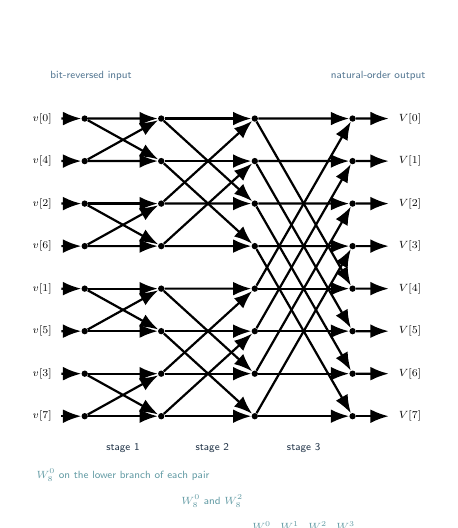
\begin{tikzpicture}[>=Latex, scale=0.54, transform shape, every node/.style={font=\scriptsize}]
    \foreach \y/\lin/\rout in {
      7/{\(v[0]\)}/{\(V[0]\)},
      6/{\(v[4]\)}/{\(V[1]\)},
      5/{\(v[2]\)}/{\(V[2]\)},
      4/{\(v[6]\)}/{\(V[3]\)},
      3/{\(v[1]\)}/{\(V[4]\)},
      2/{\(v[5]\)}/{\(V[5]\)},
      1/{\(v[3]\)}/{\(V[6]\)},
      0/{\(v[7]\)}/{\(V[7]\)}
    }{
      \node at (0,\y) {\lin};
      \node[fftdot] (szero\y) at (1.0,\y) {};
      \node[fftdot] (sone\y) at (2.8,\y) {};
      \node[fftdot] (stwo\y) at (5.0,\y) {};
      \node[fftdot] (sthree\y) at (7.3,\y) {};
      \node at (8.65,\y) {\rout};
      \draw[->, thick] (0.45,\y)--(szero\y);
      \draw[->, thick] (sthree\y)--(8.15,\y);
    }
    \foreach \a/\b in {7/6,5/4,3/2,1/0} {
      \draw[->, thick] (szero\a)--(sone\a);
      \draw[->, thick] (szero\b)--(sone\b);
      \draw[->, thick] (szero\a)--(sone\b);
      \draw[->, thick] (szero\b)--(sone\a);
    }
    \foreach \a/\b/\c/\d in {7/6/5/4,3/2/1/0} {
      \draw[->, thick] (sone\a)--(stwo\a);
      \draw[->, thick] (sone\b)--(stwo\b);
      \draw[->, thick] (sone\c)--(stwo\c);
      \draw[->, thick] (sone\d)--(stwo\d);
      \draw[->, thick] (sone\a)--(stwo\c);
      \draw[->, thick] (sone\c)--(stwo\a);
      \draw[->, thick] (sone\b)--(stwo\d);
      \draw[->, thick] (sone\d)--(stwo\b);
    }
    \foreach \a/\b in {7/3,6/2,5/1,4/0} {
      \draw[->, thick] (stwo\a)--(sthree\a);
      \draw[->, thick] (stwo\b)--(sthree\b);
      \draw[->, thick] (stwo\a)--(sthree\b);
      \draw[->, thick] (stwo\b)--(sthree\a);
    }
    \node[SecondaryColor] at (1.15,8.0) {bit-reversed input};
    \node[SecondaryColor] at (7.9,8.0) {natural-order output};
    \node[PrimaryColor] at (1.9,-0.75) {stage 1};
    \node[PrimaryColor] at (4.0,-0.75) {stage 2};
    \node[PrimaryColor] at (6.15,-0.75) {stage 3};
    \node[AccentColor] at (1.9,-1.38) {\(W_8^0\) on the lower branch of each pair};
    \node[AccentColor] at (4.0,-2.0) {\(W_8^0\) and \(W_8^2\)};
    \node[AccentColor] at (6.15,-2.62) {\(W_8^0,\ W_8^1,\ W_8^2,\ W_8^3\)};
  \end{tikzpicture}%
}

\begin{document}

\begin{center}
  {\LARGE \textbf{CSE 219 Practice Sheet}}\\[0.24em]
  {\large FFT, Sampling, Laplace Transform, and z-Transform}\\[1em]
  {\normalfont Ashrafur Rahman\\ Lecturer, CSE, BUET}
\end{center}

\vspace{2cm}

\tableofcontents

\vspace{5cm}
\newpage

\section{Radix-2 DIT Cooley-Tukey FFT}

\begin{examplebox}{Problem 1.1}
  \Prompt{Starting from \(X[k]=\sum_{n=0}^{N-1}x[n]W_N^{kn}\), derive the radix-2 DIT split into even and odd subsequences and the butterfly relations for \(0\le k<N/2\).}

  \medskip
  \SketchLabel{}
  Splitting \(n=2r\) and \(n=2r+1\),
  \[
    X[k]=\sum_{r=0}^{N/2-1}x[2r]W_{N/2}^{kr}+W_N^k\sum_{r=0}^{N/2-1}x[2r+1]W_{N/2}^{kr}
    =G[k]+W_N^kH[k].
  \]
  Using \(W_N^{k+N/2}=-W_N^k\),
  \[
    X[k+N/2]=G[k]-W_N^kH[k], \qquad 0\le k<\frac{N}{2}.
  \]

  \begin{center}
    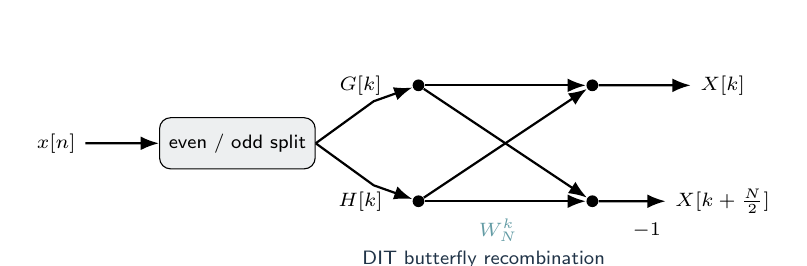
\begin{tikzpicture}[>=Latex, scale=0.92, every node/.style={font=\scriptsize}]
      \node (x) at (0,1.5) {$x[n]$};
      \node[draw, rounded corners, fill=PrimaryColor!8, minimum width=1.95cm, minimum height=0.65cm] (split) at (2.5,1.5) {even / odd split};
      \node at (4.2,2.3) {$G[k]$};
      \node at (4.2,0.7) {$H[k]$};
      \node[fftdot] (g0) at (5.0,2.3) {};
      \node[fftdot] (h0) at (5.0,0.7) {};
      \node[fftdot] (o0) at (7.4,2.3) {};
      \node[fftdot] (o1) at (7.4,0.7) {};
      \node (xk) at (9.2,2.3) {$X[k]$};
      \node (xk2) at (9.2,0.7) {$X[k+\frac N2]$};
      \draw[->, thick] (x)--(split);
      \draw[->, thick] (split.east) -- ++(0.8,0.58) -- (g0);
      \draw[->, thick] (split.east) -- ++(0.8,-0.58) -- (h0);
      \draw[->, thick] (g0)--(o0);
      \draw[->, thick] (h0)--(o1);
      \draw[->, thick] (g0)--(o1);
      \draw[->, thick] (h0)--(o0);
      \draw[->, thick] (o0)--(xk);
      \draw[->, thick] (o1)--(xk2);
      \node[AccentColor] at (6.1,0.3) {$W_N^k$};
      \node at (8.15,0.3) {$-1$};
      \node[PrimaryColor] at (5.9,-0.1) {DIT butterfly recombination};
    \end{tikzpicture}
  \end{center}
\end{examplebox}

\begin{examplebox}{Problem 1.2}
  \Prompt{Compute the 4-point DIT FFT of \(x[n]=[2,1,-3,4]\) using radix-2 butterflies.}

  \medskip
  \SketchLabel{}
  \[
    x_e=[2,-3], \qquad x_o=[1,4].
  \]
  The two 2-point DFTs are
  \[
    G=[-1,5], \qquad H=[5,-3].
  \]
  Now combine with
  \[
    X[k]=G[k]+W_4^kH[k], \qquad X[k+2]=G[k]-W_4^kH[k], \qquad k=0,1.
  \]
  For \(k=0\),
  \[
    X[0]=-1+5=4, \qquad X[2]=-1-5=-6.
  \]
  For \(k=1\), \(W_4^1=-j\), so
  \[
    X[1]=5+(-j)(-3)=5+3j, \qquad X[3]=5-(-j)(-3)=5-3j.
  \]
  Hence
  \[
    X[k]=[4,\ 5+3j,\ -6,\ 5-3j].
  \]

  \begin{center}
    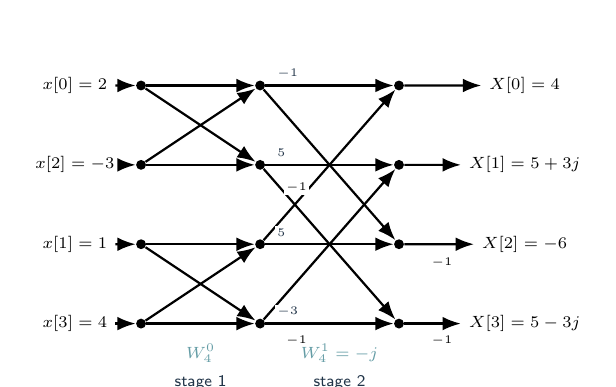
\begin{tikzpicture}[>=Latex, scale=0.84, transform shape, every node/.style={font=\scriptsize}]
      \node (x0) at (0,3.6) {$x[0]=2$};
      \node (x2) at (0,2.4) {$x[2]=-3$};
      \node (x1) at (0,1.2) {$x[1]=1$};
      \node (x3) at (0,0.0) {$x[3]=4$};
      \node[fftdot] (a0) at (1.0,3.6) {};
      \node[fftdot] (a1) at (1.0,2.4) {};
      \node[fftdot] (a2) at (1.0,1.2) {};
      \node[fftdot] (a3) at (1.0,0.0) {};
      \node[fftdot] (b0) at (2.8,3.6) {};
      \node[fftdot] (b1) at (2.8,2.4) {};
      \node[fftdot] (b2) at (2.8,1.2) {};
      \node[fftdot] (b3) at (2.8,0.0) {};
      \node[fftdot] (c0) at (4.9,3.6) {};
      \node[fftdot] (c1) at (4.9,2.4) {};
      \node[fftdot] (c2) at (4.9,1.2) {};
      \node[fftdot] (c3) at (4.9,0.0) {};
      \node (X0) at (6.8,3.6) {$X[0]=4$};
      \node (X1) at (6.8,2.4) {$X[1]=5+3j$};
      \node (X2) at (6.8,1.2) {$X[2]=-6$};
      \node (X3) at (6.8,0.0) {$X[3]=5-3j$};

      \draw[->, thick] (x0)--(a0);
      \draw[->, thick] (x2)--(a1);
      \draw[->, thick] (x1)--(a2);
      \draw[->, thick] (x3)--(a3);

      \draw[->, thick] (a0)--(b0);
      \draw[->, thick] (a1)--(b1);
      \draw[->, thick] (a0)--(b1);
      \draw[->, thick] (a1)--(b0);
      \draw[->, thick] (a2)--(b2);
      \draw[->, thick] (a3)--(b3);
      \draw[->, thick] (a2)--(b3);
      \draw[->, thick] (a3)--(b2);

      \draw[->, thick] (b0)--(c0);
      \draw[->, thick] (b2)--(c2);
      \draw[->, thick] (b0)--(c2);
      \draw[->, thick] (b2)--(c0);
      \draw[->, thick] (b1)--(c1);
      \draw[->, thick] (b3)--(c3);
      \draw[->, thick] (b1)--(c3);
      \draw[->, thick] (b3)--(c1);

      \draw[->, thick] (c0)--(X0);
      \draw[->, thick] (c1)--(X1);
      \draw[->, thick] (c2)--(X2);
      \draw[->, thick] (c3)--(X3);

      \node[fftvalue, anchor=west] at (3.02,3.78) {$-1$};
      \node[fftvalue, anchor=west] at (3.02,2.58) {$5$};
      \node[fftvalue, anchor=west] at (3.02,1.38) {$5$};
      \node[fftvalue, anchor=west] at (3.02,0.18) {$-3$};
      \node[font=\tiny, fill=white, inner sep=1pt] at (3.35,2.06) {$-1$};
      \node[font=\tiny, fill=white, inner sep=1pt] at (3.35,-0.26) {$-1$};
      \node[font=\tiny, fill=white, inner sep=1pt] at (5.55,0.92) {$-1$};
      \node[font=\tiny, fill=white, inner sep=1pt] at (5.55,-0.26) {$-1$};

      \node[AccentColor] at (1.9,-0.45) {\(W_4^0\)};
      \node[AccentColor] at (4.0,-0.45) {\(W_4^1=-j\)};
      \node[PrimaryColor] at (1.9,-0.9) {stage 1};
      \node[PrimaryColor] at (4.0,-0.9) {stage 2};
    \end{tikzpicture}
  \end{center}
\end{examplebox}

\newpage

\begin{examplebox}{Problem 1.3}
  \Prompt{Compute the 4-point FFT of \(x[n]=[1,2,3,4]\) using two 2-point butterflies.}

  \medskip
  \SketchLabel{}
  Split into even and odd subsequences:
  \[
    x_e=[1,3], \qquad x_o=[2,4].
  \]
  Their 2-point DFTs are \(G=[4,-2]\) and \(H=[6,-2]\). Therefore
  \[
    X[0]=10,\quad X[1]=-2+2j,\quad X[2]=-2,\quad X[3]=-2-2j.
  \]

  \begin{center}
    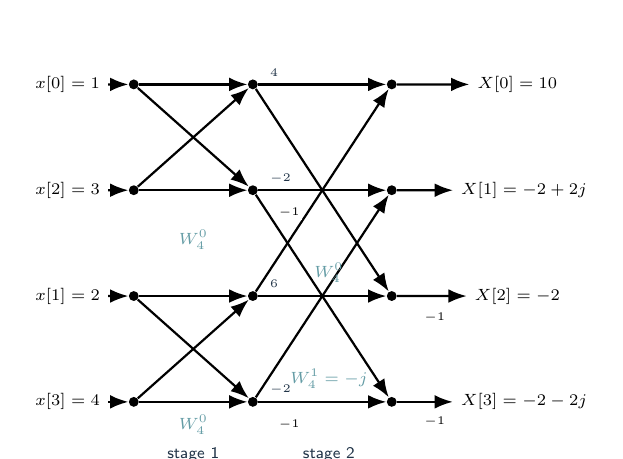
\begin{tikzpicture}[>=Latex, scale=0.84, transform shape, every node/.style={font=\scriptsize}]
      \node (x0) at (0, 4.8) {$x[0]=1$};
      \node (x2) at (0, 3.2) {$x[2]=3$};
      \node (x1) at (0, 1.6) {$x[1]=2$};
      \node (x3) at (0, 0.0) {$x[3]=4$};
      \node[fftdot] (a0) at (1.0,4.8) {};
      \node[fftdot] (a1) at (1.0,3.2) {};
      \node[fftdot] (a2) at (1.0,1.6) {};
      \node[fftdot] (a3) at (1.0,0.0) {};
      \node[fftdot] (b0) at (2.8,4.8) {};
      \node[fftdot] (b1) at (2.8,3.2) {};
      \node[fftdot] (b2) at (2.8,1.6) {};
      \node[fftdot] (b3) at (2.8,0.0) {};
      \node[fftdot] (c0) at (4.9,4.8) {};
      \node[fftdot] (c1) at (4.9,3.2) {};
      \node[fftdot] (c2) at (4.9,1.6) {};
      \node[fftdot] (c3) at (4.9,0.0) {};
      \node (X0) at (6.8,4.8) {$X[0]=10$};
      \node (X1) at (6.9,3.2) {$X[1]=-2+2j$};
      \node (X2) at (6.8,1.6) {$X[2]=-2$};
      \node (X3) at (6.9,0.0) {$X[3]=-2-2j$};

      \draw[->, thick] (x0)--(a0);
      \draw[->, thick] (x2)--(a1);
      \draw[->, thick] (x1)--(a2);
      \draw[->, thick] (x3)--(a3);

      \draw[->, thick] (a0)--(b0);
      \draw[->, thick] (a1)--(b1);
      \draw[->, thick] (a0)--(b1);
      \draw[->, thick] (a1)--(b0);
      \draw[->, thick] (a2)--(b2);
      \draw[->, thick] (a3)--(b3);
      \draw[->, thick] (a2)--(b3);
      \draw[->, thick] (a3)--(b2);

      \draw[->, thick] (b0)--(c0);
      \draw[->, thick] (b2)--(c2);
      \draw[->, thick] (b0)--(c2);
      \draw[->, thick] (b2)--(c0);
      \draw[->, thick] (b1)--(c1);
      \draw[->, thick] (b3)--(c3);
      \draw[->, thick] (b1)--(c3);
      \draw[->, thick] (b3)--(c1);

      \draw[->, thick] (c0)--(X0);
      \draw[->, thick] (c1)--(X1);
      \draw[->, thick] (c2)--(X2);
      \draw[->, thick] (c3)--(X3);

      \node[fftvalue, anchor=west] at (3.02,4.98) {$4$};
      \node[fftvalue, anchor=west] at (3.02,3.38) {$-2$};
      \node[fftvalue, anchor=west] at (3.02,1.78) {$6$};
      \node[fftvalue, anchor=west] at (3.02,0.18) {$-2$};

      \node[AccentColor] at (1.9,2.45) {$W_4^0$};
      \node[AccentColor] at (1.9,-0.35) {$W_4^0$};
      \node[font=\tiny, fill=white, inner sep=1pt] at (3.35,2.86) {$-1$};
      \node[font=\tiny, fill=white, inner sep=1pt] at (3.35,-0.35) {$-1$};
      \node[AccentColor] at (3.95,1.95) {$W_4^0$};
      \node[AccentColor] at (3.95,0.35) {$W_4^1=-j$};
      \node[font=\tiny, fill=white, inner sep=1pt] at (5.55,1.28) {$-1$};
      \node[font=\tiny, fill=white, inner sep=1pt] at (5.55,-0.30) {$-1$};

      \node[PrimaryColor] at (1.9,-0.8) {stage 1};
      \node[PrimaryColor] at (3.95,-0.8) {stage 2};
    \end{tikzpicture}
  \end{center}
\end{examplebox}

\begin{examplebox}{Problem 1.4}
  \Prompt{Compute the 8-point FFT of \(x[n]=[1,2,0,-1,3,0,2,1]\) using the full radix-2 DIT butterfly.}

  \medskip
  \SketchLabel{}
  For an iterative radix-2 DIT flow, place the data in bit-reversed order:
  \[
    [x[0],x[4],x[2],x[6],x[1],x[5],x[3],x[7]]
    =[1,3,0,2,2,0,-1,1].
  \]
  After the first butterfly stage,
  \[
    [4,\,-2,\ 2,\,-2,\ 2,\ 2,\ 0,\,-2].
  \]
  After the second stage,
  \[
    [6,\,-2+2j,\ 2,\,-2-2j,\ 2,\ 2+2j,\ 2,\ 2-2j].
  \]
  Now use the final twiddle factors \(W_8^k\), \(k=0,1,2,3\):
  \[
    \begin{aligned}
      X[0]&=6+W_8^0(2)=8,\\
      X[1]&=(-2+2j)+W_8^1(2+2j)=(-2+2j)+2\sqrt2= -2+2\sqrt2+2j,\\
      X[2]&=2+W_8^2(2)=2-2j,\\
      X[3]&=(-2-2j)+W_8^3(2-2j)= -2-2\sqrt2-2j,
    \end{aligned}
  \]
  and
  \[
    \begin{aligned}
      X[4]&=6-W_8^0(2)=4,\\
      X[5]&=(-2+2j)-W_8^1(2+2j)= -2-2\sqrt2+2j,\\
      X[6]&=2-W_8^2(2)=2+2j,\\
      X[7]&=(-2-2j)-W_8^3(2-2j)= -2+2\sqrt2-2j.
    \end{aligned}
  \]
  So the final 8-point FFT is
  \[
    \begin{aligned}
      X[k]=[&8,\ -2+2\sqrt2+2j,\ 2-2j,\ -2-2\sqrt2-2j,\\
      &4,\ -2-2\sqrt2+2j,\ 2+2j,\ -2+2\sqrt2-2j ].
    \end{aligned}
  \]

  \begin{center}
    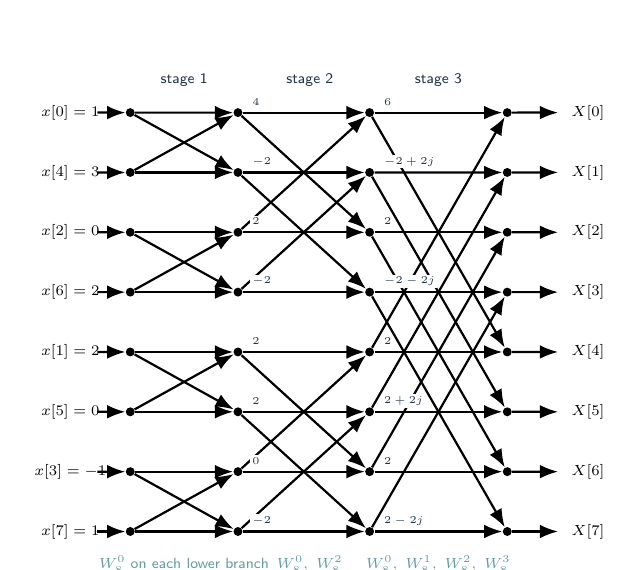
\begin{tikzpicture}[>=Latex, scale=0.76, transform shape, every node/.style={font=\scriptsize}]
      \foreach \y/\label in {
        7/{\(x[0]=1\)},6/{\(x[4]=3\)},5/{\(x[2]=0\)},4/{\(x[6]=2\)},
        3/{\(x[1]=2\)},2/{\(x[5]=0\)},1/{\(x[3]=-1\)},0/{\(x[7]=1\)}
      }{
        \node at (0,\y) {\label};
        \node[fftdot] (s0\y) at (1.0,\y) {};
        \node[fftdot] (s1\y) at (2.8,\y) {};
        \node[fftdot] (s2\y) at (5.0,\y) {};
        \node[fftdot] (s3\y) at (7.3,\y) {};
      }
      \foreach \y/\label in {
        7/{\(X[0]\)},6/{\(X[1]\)},5/{\(X[2]\)},4/{\(X[3]\)},
        3/{\(X[4]\)},2/{\(X[5]\)},1/{\(X[6]\)},0/{\(X[7]\)}
      }{
        \node at (8.65,\y) {\label};
        \draw[->, thick] (s3\y)--(8.15,\y);
      }
      \foreach \y in {7,6,5,4,3,2,1,0} {
        \draw[->, thick] (0.45,\y)--(s0\y);
      }
      \foreach \a/\b in {7/6,5/4,3/2,1/0} {
        \draw[->, thick] (s0\a)--(s1\a);
        \draw[->, thick] (s0\b)--(s1\b);
        \draw[->, thick] (s0\a)--(s1\b);
        \draw[->, thick] (s0\b)--(s1\a);
      }
      \foreach \a/\b/\c/\d in {7/6/5/4,3/2/1/0} {
        \draw[->, thick] (s1\a)--(s2\a);
        \draw[->, thick] (s1\b)--(s2\b);
        \draw[->, thick] (s1\c)--(s2\c);
        \draw[->, thick] (s1\d)--(s2\d);
        \draw[->, thick] (s1\a)--(s2\c);
        \draw[->, thick] (s1\c)--(s2\a);
        \draw[->, thick] (s1\b)--(s2\d);
        \draw[->, thick] (s1\d)--(s2\b);
      }
      \foreach \a/\b in {7/3,6/2,5/1,4/0} {
        \draw[->, thick] (s2\a)--(s3\a);
        \draw[->, thick] (s2\b)--(s3\b);
        \draw[->, thick] (s2\a)--(s3\b);
        \draw[->, thick] (s2\b)--(s3\a);
      }

      \foreach \y/\val in {
        7/{4},6/{-2},5/{2},4/{-2},
        3/{2},2/{2},1/{0},0/{-2}
      }{
        \node[fftvalue, anchor=west] at (3.0,\y+0.18) {$\val$};
      }
      \foreach \y/\val in {
        7/{6},6/{-2+2j},5/{2},4/{-2-2j},
        3/{2},2/{2+2j},1/{2},0/{2-2j}
      }{
        \node[fftvalue, anchor=west] at (5.2,\y+0.18) {$\val$};
      }

      \node[PrimaryColor] at (1.9,7.55) {stage 1};
      \node[PrimaryColor] at (4.0,7.55) {stage 2};
      \node[PrimaryColor] at (6.15,7.55) {stage 3};
      \node[AccentColor] at (1.9,-0.55) {\(W_8^0\) on each lower branch};
      \node[AccentColor] at (4.0,-0.55) {\(W_8^0,\ W_8^2\)};
      \node[AccentColor] at (6.15,-0.55) {\(W_8^0,\ W_8^1,\ W_8^2,\ W_8^3\)};
    \end{tikzpicture}
  \end{center}
\end{examplebox}

\begin{examplebox}{Problem 1.5}
  \Prompt{Recover \(x[n]\) from
    \[
      X[k]=[\,6,\ \sqrt2-j\sqrt2,\ 2+4j,\ -\sqrt2-j\sqrt2,\ -2,\ -\sqrt2+j\sqrt2,\ 2-4j,\ \sqrt2+j\sqrt2\,]
    \]
  using an 8-point inverse FFT.}

  \medskip
  \SketchLabel{}
  Use the same radix-2 DIT butterfly graph as the forward 8-point FFT, but replace each lower-branch twiddle by \(W_8^{-k}\) and divide the final output by \(8\).
  Feed the samples in bit-reversed order:
  \[
    [X[0],X[4],X[2],X[6],X[1],X[5],X[3],X[7]]
    =[\,6,\ -2,\ 2+4j,\ 2-4j,\ \sqrt2-j\sqrt2,\ -\sqrt2+j\sqrt2,\ -\sqrt2-j\sqrt2,\ \sqrt2+j\sqrt2\,].
  \]
  Stage 1 uses only \(W_8^0=1\), so
  \[
    \text{stage 1: } [\,4,\ 8,\ 4,\ 8j,\ 0,\ 2\sqrt2-2\sqrt2\,j,\ 0,\ -2\sqrt2-2\sqrt2\,j\,].
  \]
  At stage 2 the nontrivial lower-branch twiddle is \(W_8^{-2}=j\), giving
  \[
    \text{stage 2: } [\,8,\ 0,\ 0,\ 16,\ 0,\ 4\sqrt2-4\sqrt2\,j,\ 0,\ 0\,].
  \]
  At stage 3 the lower-branch twiddles are \(W_8^0,\ W_8^{-1},\ W_8^{-2},\ W_8^{-3}\), so
  \[
    \text{stage 3: } [\,8,\ 8,\ 0,\ 16,\ 8,\ -8,\ 0,\ 16\,].
  \]
  Therefore
  \[
    x[n]=\frac18[\,8,\ 8,\ 0,\ 16,\ 8,\ -8,\ 0,\ 16\,]
    =[\,1,\ 1,\ 0,\ 2,\ 1,\ -1,\ 0,\ 2\,].
  \]

  \begin{center}
    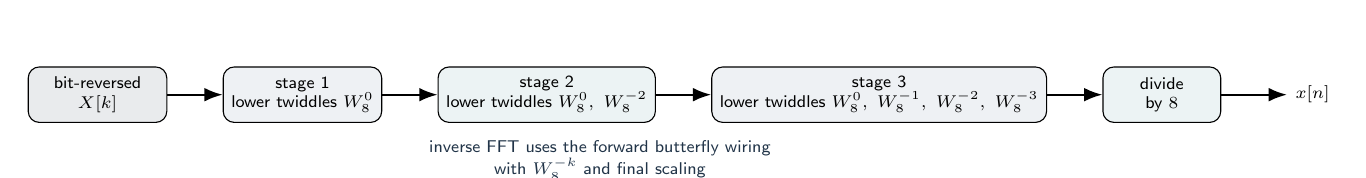
\begin{tikzpicture}[>=Latex, node distance=0.8cm, scale=0.88, transform shape, font=\scriptsize]
      \node[draw, rounded corners, fill=PrimaryColor!10, minimum width=2.0cm, minimum height=0.8cm, align=center] (a) {bit-reversed\\\(X[k]\)};
      \node[draw, rounded corners, fill=SecondaryColor!10, minimum width=2.2cm, minimum height=0.8cm, align=center, right=of a] (b) {stage 1\\lower twiddles \(W_8^0\)};
      \node[draw, rounded corners, fill=AccentColor!12, minimum width=2.5cm, minimum height=0.8cm, align=center, right=of b] (c) {stage 2\\lower twiddles \(W_8^0,\ W_8^{-2}\)};
      \node[draw, rounded corners, fill=SecondaryColor!10, minimum width=3.0cm, minimum height=0.8cm, align=center, right=of c] (d) {stage 3\\lower twiddles \(W_8^0,\ W_8^{-1},\ W_8^{-2},\ W_8^{-3}\)};
      \node[draw, rounded corners, fill=AccentColor!12, minimum width=1.7cm, minimum height=0.8cm, align=center, right=of d] (e) {divide\\by \(8\)};
      \node[right=0.95cm of e] (f) {\(x[n]\)};
      \draw[->, thick] (a)--(b);
      \draw[->, thick] (b)--(c);
      \draw[->, thick] (c)--(d);
      \draw[->, thick] (d)--(e);
      \draw[->, thick] (e)--(f);
      \node[PrimaryColor, align=center, text width=7.1cm] at (7.25,-0.95) {inverse FFT uses the forward butterfly wiring\\with \(W_8^{-k}\) and final scaling};
    \end{tikzpicture}
  \end{center}
\end{examplebox}

\section{2D Matrix Formulation of Cooley-Tukey (Bailey's FFT)}

\begin{examplebox}{Problem 2.1}
  \Prompt{Show how a 4-point DFT can be written as a \(2\times 2\) matrix factorization using column-major input, row DFTs, twiddles, and column DFTs.}

  \medskip
  \SketchLabel{}
  Arrange the samples in \emph{column-major} order so the first row contains the even-indexed samples and the second row contains the odd-indexed samples:
  \[
    \begin{bmatrix}
      x_0 & x_2\\
      x_1 & x_3
    \end{bmatrix}.
  \]
  Apply 2-point DFTs along the rows:
  \[
    \begin{bmatrix}
      x_0+x_2 & x_0-x_2\\
      x_1+x_3 & x_1-x_3
    \end{bmatrix}.
  \]
  Twiddle the second row by \([1,W_4^1]\), so only the lower-right entry picks up \(W_4^1=-j\). The matrix after twiddle multiplication is
  \[
    \begin{bmatrix}
      x_0+x_2 & x_0-x_2\\
      x_1+x_3 & -j(x_1-x_3)
    \end{bmatrix}.
  \]
  Now apply 2-point DFTs down the columns. The column-wise 2-point FFT produces
  \[
    \begin{bmatrix}
      (x_0+x_2)+(x_1+x_3) & (x_0-x_2)-j(x_1-x_3)\\
      (x_0+x_2)-(x_1+x_3) & (x_0-x_2)+j(x_1-x_3)
    \end{bmatrix}.
  \]
  Reading out this final matrix in row-major order gives
  \[
    \begin{aligned}
      X[0]&=x_0+x_1+x_2+x_3,\\
      X[1]&=(x_0-x_2)-j(x_1-x_3),\\
      X[2]&=(x_0+x_2)-(x_1+x_3),\\
      X[3]&=(x_0-x_2)+j(x_1-x_3).
    \end{aligned}
  \]

  \begin{center}
    
\begin{tikzpicture}[>=Latex, node distance=0.95cm, scale=0.92, transform shape, font=\scriptsize]
      \node[draw, rounded corners, fill=PrimaryColor!10, minimum width=1.6cm, minimum height=0.65cm] (a) {column-major\ \(2\times2\) reshape};
      \node[draw, rounded corners, fill=SecondaryColor!10, minimum width=1.7cm, minimum height=0.65cm, right=of a] (b) {row DFTs};
      \node[draw, rounded corners, fill=AccentColor!12, minimum width=1.2cm, minimum height=0.65cm, right=of b] (c) {twiddle};
      \node[draw, rounded corners, fill=SecondaryColor!10, minimum width=1.5cm, minimum height=0.65cm, right=of c] (d) {column DFTs};
      \draw[->, thick] (a)--(b);
      \draw[->, thick] (b)--(c);
      \draw[->, thick] (c)--(d);
      \node[PrimaryColor] at (3.7,-0.65) {Bailey factorization pipeline};
    \end{tikzpicture}
  \end{center}
\end{examplebox}

\newpage

\begin{examplebox}{Problem 2.2}
  \Prompt{Use a \(2\times 4\) Bailey factorization to compute the 8-point DFT of \(x[n]=[1,3,-1,2,0,4,2,1]\).}

  \medskip
  \SketchLabel{}
  Write the input in column-major order so the top row is the even-indexed subsequence and the bottom row is the odd-indexed subsequence:
  \[
    \mathbf{X}_{\text{in}}=
    \begin{bmatrix}
      1&-1&0&2\\
      3&2&4&1
    \end{bmatrix}.
  \]
  First apply a 4-point DFT to each row:
  \[
    \mathbf{R}=
    \begin{bmatrix}
      2&1+3j&0&1-3j\\
      10&-1-j&4&-1+j
    \end{bmatrix}.
  \]
  Now twiddle the second row by \([1,W_8^1,W_8^2,W_8^3]\):
  \[
    \mathbf{T}=
    \begin{bmatrix}
      2&1+3j&0&1-3j\\
      10&(-1-j)W_8^1&4W_8^2&(-1+j)W_8^3
    \end{bmatrix}
    =
    \begin{bmatrix}
      2&1+3j&0&1-3j\\
      10&-\sqrt2&-4j&\sqrt2
    \end{bmatrix}.
  \]
  Finally apply 2-point DFTs down each column:
  \[
    \begin{aligned}
      X[0]&=2+10=12, & X[4]&=2-10=-8,\\
      X[1]&=(1+3j)-\sqrt2=1-\sqrt2+3j, & X[5]&=(1+3j)+\sqrt2=1+\sqrt2+3j,\\
      X[2]&=0-4j=-4j, & X[6]&=0-(-4j)=4j,\\
      X[3]&=(1-3j)+\sqrt2=1+\sqrt2-3j, & X[7]&=(1-3j)-\sqrt2=1-\sqrt2-3j.
    \end{aligned}
  \]
  The final matrix is read out in \emph{row-major} order, so we obtain
  \[
    \begin{aligned}
      X[0]&=12,& X[1]&=1-\sqrt2+3j,& X[2]&=-4j,& X[3]&=1+\sqrt2-3j,\\
      X[4]&=-8,& X[5]&=1+\sqrt2+3j,& X[6]&=4j,& X[7]&=1-\sqrt2-3j.
    \end{aligned}
  \]

  \begin{center}
    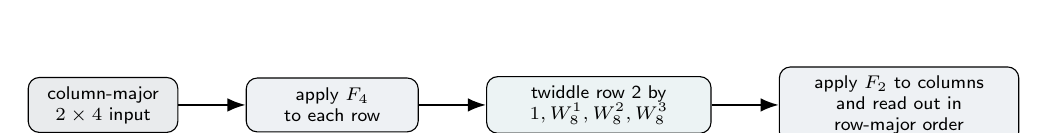
\begin{tikzpicture}[>=Latex, node distance=0.9cm, scale=0.95, transform shape, font=\scriptsize]
      \node[draw, rounded corners, fill=PrimaryColor!10, minimum width=2.0cm, minimum height=0.72cm, align=center] (a) {column-major\\ \(2\times 4\) input};
      \node[draw, rounded corners, fill=SecondaryColor!10, minimum width=2.3cm, minimum height=0.72cm, align=center, right=of a] (b) {apply \(F_4\)\\to each row};
      \node[draw, rounded corners, fill=AccentColor!12, minimum width=3.0cm, minimum height=0.72cm, align=center, right=of b] (c) {twiddle row 2 by\\ \(1,W_8^1,W_8^2,W_8^3\)};
      \node[draw, rounded corners, fill=SecondaryColor!10, minimum width=3.2cm, minimum height=0.72cm, align=center, right=of c] (d) {apply \(F_2\) to columns\\and read out in\\row-major order};
      \draw[->, thick] (a)--(b);
      \draw[->, thick] (b)--(c);
      \draw[->, thick] (c)--(d);
    \end{tikzpicture}
  \end{center}
\end{examplebox}

\begin{examplebox}{Problem 2.3}
  \Prompt{A 16-point sequence is \(x[n]=[1,0,0,0,\,2,0,0,0,\,-1,0,0,0,\,3,0,0,0]\). Use the \(4\times 4\) formulation to reduce the work.}

  \medskip
  \SketchLabel{}
  Write the sequence in column-major form so row \(r\) collects samples with indices \(n\equiv r\pmod 4\):
  \[
    \begin{bmatrix}
      1&2&-1&3\\
      0&0&0&0\\
      0&0&0&0\\
      0&0&0&0
    \end{bmatrix}.
  \]
  Only the first row is active. The row-stage 4-point DFT therefore acts only on
  \[
    [1,\ 2,\ -1,\ 3],
  \]
  giving
  \[
    [5,\ 2+j,\ -5,\ 2-j].
  \]
  So after the row DFTs,
  \[
    \mathbf{R}=
    \begin{bmatrix}
      5&2+j&-5&2-j\\
      0&0&0&0\\
      0&0&0&0\\
      0&0&0&0
    \end{bmatrix}.
  \]
  The twiddle matrix does nothing here, because only row \(r=0\) survives and \(W_{16}^{rk}=W_{16}^{0}=1\).
  Now each column has the form \([a,0,0,0]^T\), whose 4-point DFT is simply \([a,a,a,a]^T\). Hence
  \[
    \mathbf{C}=
    \begin{bmatrix}
      5&2+j&-5&2-j\\
      5&2+j&-5&2-j\\
      5&2+j&-5&2-j\\
      5&2+j&-5&2-j
    \end{bmatrix}.
  \]
  Read out the matrix in row-major order,
  \[
    X[k]=[5,\ 2+j,\ -5,\ 2-j,\ 5,\ 2+j,\ -5,\ 2-j,\ 5,\ 2+j,\ -5,\ 2-j,\ 5,\ 2+j,\ -5,\ 2-j].
  \]

  \begin{center}
    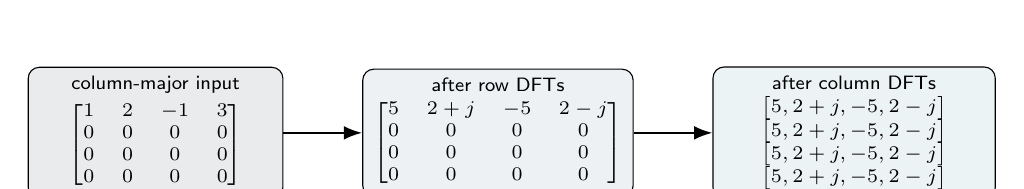
\begin{tikzpicture}[>=Latex, node distance=1.0cm, font=\scriptsize]
      \node[draw, rounded corners, fill=PrimaryColor!10, align=center, text width=3.0cm] (a) {column-major input\\[0.2em]
        \(
          \begin{bmatrix}1&2&-1&3\\0&0&0&0\\0&0&0&0\\0&0&0&0
      \end{bmatrix}\)};
      \node[draw, rounded corners, fill=SecondaryColor!10, align=center, text width=3.2cm, right=of a] (b) {after row DFTs\\[0.2em]
        \(
          \begin{bmatrix}5&2+j&-5&2-j\\0&0&0&0\\0&0&0&0\\0&0&0&0
      \end{bmatrix}\)};
      \node[draw, rounded corners, fill=AccentColor!12, align=center, text width=3.35cm, right=of b] (c) {after column DFTs\\[0.2em]
        \(
          \begin{array}{c}
            \bigl[5,2+j,-5,2-j\bigr]\\
            \bigl[5,2+j,-5,2-j\bigr]\\
            \bigl[5,2+j,-5,2-j\bigr]\\
            \bigl[5,2+j,-5,2-j\bigr]
      \end{array}\)};
      \draw[->, thick] (a)--(b);
      \draw[->, thick] (b)--(c);
    \end{tikzpicture}
  \end{center}
\end{examplebox}

\section{Bluestein's FFT}

\begin{examplebox}{Problem 3.1}
  \Prompt{Derive Bluestein's chirp identity
    \[
      W_N^{nk}=W_{2N}^{-(k-n)^2}W_{2N}^{k^2}W_{2N}^{n^2}.
  \]}

  \medskip
  \SketchLabel{}
  Since
  \[
    (k-n)^2=k^2-2kn+n^2,
  \]
  we get
  \[
    kn=-\frac{(k-n)^2}{2}+\frac{k^2}{2}+\frac{n^2}{2}.
  \]
  Because \(W_N^{nk}=W_{2N}^{2nk}\), substitution gives
  \[
    X[k]
    =\sum_{n=0}^{N-1}x[n]W_{2N}^{-(k-n)^2}W_{2N}^{k^2}W_{2N}^{n^2}
    =W_{2N}^{k^2}\sum_{n=0}^{N-1}a[n]\,b[k-n],
  \]
  where \(a[n]=x[n]W_{2N}^{n^2}\) and \(b[m]=W_{2N}^{-m^2}\). Thus the DFT becomes a chirp-weighted linear convolution.
  For the needed outputs \(0\le k\le N-1\) and data indices \(0\le n\le N-1\), the difference
  \[
    m=k-n
  \]
  runs from \(-(N-1)\) to \(N-1\). So \(b[m]\) must be available on exactly \(2N-1\) consecutive indices. That is why Bluestein needs an FFT length
  \[
    M\ge 2N-1,
  \]
  usually the next radix-2 choice. In a packed FFT buffer, \(a[n]\) sits in slots \(0,\dots,N-1\), while \(b[m]\) is stored as
  \[
    [\,b[0],b[1],\dots,b[N-1],0,\dots,0,b[-(N-1)],\dots,b[-1]\,].
  \]

  \begin{center}
    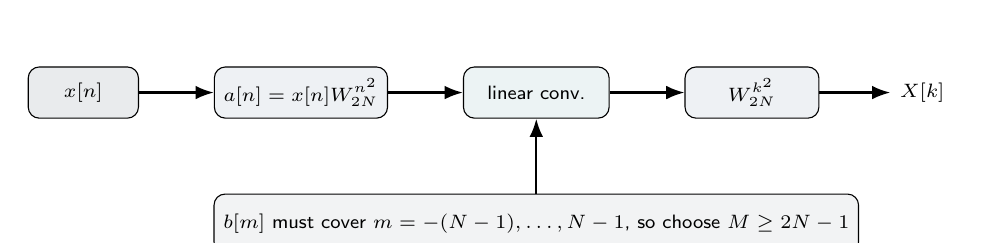
\begin{tikzpicture}[>=Latex, node distance=0.95cm, font=\scriptsize]
      \node[draw, rounded corners, fill=PrimaryColor!10, minimum width=1.4cm, minimum height=0.65cm] (a) {$x[n]$};
      \node[draw, rounded corners, fill=SecondaryColor!10, minimum width=1.7cm, minimum height=0.65cm, right=of a] (b) {\(a[n]=x[n]W_{2N}^{n^2}\)};
      \node[draw, rounded corners, fill=AccentColor!12, minimum width=1.85cm, minimum height=0.65cm, right=of b] (c) {linear conv.};
      \node[draw, rounded corners, fill=SecondaryColor!10, minimum width=1.7cm, minimum height=0.65cm, right=of c] (d) {\(W_{2N}^{k^2}\)};
      \node[right=0.9cm of d] (e) {$X[k]$};
      \draw[->, thick] (a)--(b);
      \draw[->, thick] (b)--(c);
      \draw[->, thick] (c)--(d);
      \draw[->, thick] (d)--(e);
      \node[draw, rounded corners, fill=PrimaryColor!6, minimum width=4.9cm, minimum height=0.75cm, below=0.95cm of c] (f) {\(b[m]\) must cover \(m=-(N-1),\dots,N-1\), so choose \(M\ge 2N-1\)};
      \draw[->, thick] (f.north)--(c.south);
    \end{tikzpicture}
  \end{center}
\end{examplebox}

\begin{examplebox}{Problem 3.2}
  \Prompt{Use Bluestein's construction to compute the 3-point DFT of \(x[n]=[2,-1,3]\).}

  \medskip
  \SketchLabel{}
  Let \(W_6=e^{-j\pi/3}\). Bluestein writes
  \[
    X[k]=W_6^{k^2}c[k],\qquad
    c[k]=\sum_{n=0}^{2}a[n]\,b[k-n],
  \]
  with
  \[
    a[n]=x[n]W_6^{n^2}=[2,\ -W_6,\ 3W_6^4]
    =\left[2,\ -\frac12+\frac{\sqrt3}{2}j,\ -\frac32+\frac{3\sqrt3}{2}j\right].
  \]
  Also,
  \[
    b[m]=W_6^{-m^2},\qquad m=-2,-1,0,1,2,
  \]
  so
  \[
    [b[-2],b[-1],b[0],b[1],b[2]]
    =[W_6^{-4},\,W_6^{-1},\,1,\,W_6^{-1},\,W_6^{-4}].
  \]
  Because \(2N-1=5\), a radix-2 implementation uses \(M=8\) and may pack
  \[
    A=[\,2,\ -W_6,\ 3W_6^4,\ 0,\ 0,\ 0,\ 0,\ 0\,],
  \]
  \[
    B=[\,1,\ W_6^{-1},\ W_6^{-4},\ 0,\ 0,\ 0,\ W_6^{-4},\ W_6^{-1}\,].
  \]
  Now evaluate the needed convolution samples:
  \[
    \begin{aligned}
      c[0]&=2\cdot 1+(-W_6)W_6^{-1}+3W_6^4W_6^{-4}=2-1+3=4,\\
      c[1]&=2W_6^{-1}+(-W_6)\cdot 1+3W_6^4W_6^{-1}
      =2W_6^{-1}-W_6+3W_6^3
      =-\frac52+\frac{3\sqrt3}{2}j,\\
      c[2]&=2W_6^{-4}+(-W_6)W_6^{-1}+3W_6^4\cdot 1
      =2W_6^2-1+3W_6^4
      =-\frac72+\frac{\sqrt3}{2}j.
    \end{aligned}
  \]
  Finally,
  \[
    \begin{aligned}
      X[0]&=W_6^0c[0]=4,\\
      X[1]&=W_6c[1]
      =\left(\frac12-\frac{\sqrt3}{2}j\right)\left(-\frac52+\frac{3\sqrt3}{2}j\right)
      =1+2\sqrt3\,j,\\
      X[2]&=W_6^4c[2]
      =\left(-\frac12+\frac{\sqrt3}{2}j\right)\left(-\frac72+\frac{\sqrt3}{2}j\right)
      =1-2\sqrt3\,j.
    \end{aligned}
  \]

  % \begin{center}
  %   \begin{tikzpicture}[>=Latex, font=\scriptsize]
  %     \draw[PrimaryColor, thick] (0,0.35) rectangle (2.4,1.25);
  %     \node at (1.2,0.8) {\(x[n]\)};
  %     \draw[->, thick, SecondaryColor] (2.55,0.8)--(3.7,0.8);
  %     \draw[PrimaryColor, thick] (3.9,0.35) rectangle (6.3,1.25);
  %     \node at (5.1,0.8) {\(a[n]=x[n]W_6^{n^2}\)};
  %     \draw[->, thick, SecondaryColor] (6.45,0.8)--(7.6,0.8);
  %     \draw[PrimaryColor, thick] (7.8,0.35) rectangle (10.0,1.25);
  %     \node at (8.9,0.8) {\(c[k]=a\ast b\)};
  %     \draw[PrimaryColor, thick] (7.8,-0.95) rectangle (10.0,-0.05);
  %     \node at (8.9,-0.5) {\(b[m]=W_6^{-m^2}\)};
  %     \draw[->, thick, SecondaryColor] (8.9,-0.05)--(8.9,0.35);
  %     \draw[->, thick, SecondaryColor] (10.15,0.8)--(11.35,0.8);
  %     \draw[PrimaryColor, thick] (11.55,0.35) rectangle (13.85,1.25);
  %     \node at (12.7,0.8) {\(X[k]=W_6^{k^2}c[k]\)};
  %   \end{tikzpicture}
  % \end{center}
\end{examplebox}

\begin{examplebox}{Problem 3.3}
  \Prompt{Run the same method on the 4-point sequence \(x[n]=[1,2,0,0]\) and compare with the ordinary 4-point DFT.}

  \medskip
  \SketchLabel{}
  Let \(W_8=e^{-j\pi/4}\). Then
  \[
    X[k]=W_8^{k^2}c[k],\qquad
    a[n]=x[n]W_8^{n^2}=[1,\ 2W_8,\ 0,\ 0].
  \]
  The chirp is \(b[m]=W_8^{-m^2}\), so for \(m=-3,\ldots,3\),
  \[
    [b[-3],b[-2],b[-1],b[0],b[1],b[2],b[3]]
    =[W_8^{-1},\ -1,\ W_8^{-1},\ 1,\ W_8^{-1},\ -1,\ W_8^{-1}].
  \]
  Here \(2N-1=7\), so the usual radix-2 choice is \(M=8\), with packed buffers
  \[
    A=[\,1,\ 2W_8,\ 0,\ 0,\ 0,\ 0,\ 0,\ 0\,],
  \]
  \[
    B=[\,1,\ W_8^{-1},\ -1,\ W_8^{-1},\ 0,\ W_8^{-1},\ -1,\ W_8^{-1}\,].
  \]
  Only \(a[0]\) and \(a[1]\) are nonzero, hence
  \[
    c[k]=a[0]b[k]+a[1]b[k-1],\qquad 0\le k\le 3.
  \]
  Therefore
  \[
    \begin{aligned}
      c[0]&=1\cdot 1+2W_8\cdot W_8^{-1}=3,\\
      c[1]&=W_8^{-1}+2W_8
      =\frac{3\sqrt2}{2}-\frac{\sqrt2}{2}j,\\
      c[2]&=-1+2W_8W_8^{-1}=1,\\
      c[3]&=W_8^{-1}-2W_8
      =-\frac{\sqrt2}{2}+\frac{3\sqrt2}{2}j.
    \end{aligned}
  \]
  Multiplying by the output chirp gives
  \[
    \begin{aligned}
      X[0]&=c[0]=3,\\
      X[1]&=W_8c[1]=1-2j,\\
      X[2]&=W_8^4c[2]=-1,\\
      X[3]&=W_8^9c[3]=W_8c[3]=1+2j.
    \end{aligned}
  \]
  The ordinary 4-point DFT agrees term by term:
  \[
    \begin{aligned}
      X[0]&=1+2=3,\\
      X[1]&=1+2W_4=1-2j,\\
      X[2]&=1+2W_4^2=-1,\\
      X[3]&=1+2W_4^3=1+2j.
    \end{aligned}
  \]

\end{examplebox}

\newpage

\section{Application of FFT: Fast Convolution}

\begin{examplebox}{Problem 4.1}
  \Prompt{Compute the linear convolution of \(x[n]=[1,2]\) and \(h[n]=[1,-1]\) using a 4-point FFT.}

  \medskip
  \SketchLabel{}
  The output length is \(2+2-1=3\), so a 4-point FFT is sufficient. Zero-pad both signals to length \(4\):
  \[
    x_p[n]=[1,2,0,0],\qquad h_p[n]=[1,-1,0,0].
  \]
  For \(x_p[n]\),
  \[
    G_x=\operatorname{FFT}_2([1,0])=[1,1],\qquad H_x=\operatorname{FFT}_2([2,0])=[2,2].
  \]
  So the 4-point FFT is
  \[
    X[k]=[\,3,\ 1-2j,\ -1,\ 1+2j\,].
  \]
  For \(h_p[n]\),
  \[
    G_h=\operatorname{FFT}_2([1,0])=[1,1],\qquad H_h=\operatorname{FFT}_2([-1,0])=[-1,-1],
  \]
  so
  \[
    H[k]=[\,0,\ 1+j,\ 2,\ 1-j\,].
  \]
  Pointwise multiplication gives
  \[
    Y[k]=X[k]H[k]=[\,0,\ 3-j,\ -2,\ 3+j\,].
  \]
  For the inverse 4-point FFT, use the same butterfly wiring with \(W_4^{-k}\), then divide by \(4\). In bit-reversed order,
  \[
    [Y[0],Y[2],Y[1],Y[3]]=[\,0,\ -2,\ 3-j,\ 3+j\,].
  \]
  The inverse stages are
  \[
    \text{stage 1: }[-2,\ 2,\ 6,\ -2j],
    \qquad
    \text{stage 2: }[4,\ 4,\ -8,\ 0].
  \]
  Therefore
  \[
    y_p[n]=\frac14[\,4,\ 4,\ -8,\ 0\,]=[\,1,\ 1,\ -2,\ 0\,].
  \]
  Discard the padded zero and keep the linear-convolution part:
  \[
    y[n]=[1,\ 1,\ -2].
  \]
\end{examplebox}

\begin{examplebox}{Problem 4.2}
  \Prompt{Compute the linear convolution of \(x[n]=[1,-1,2]\) and \(h[n]=[2,1]\) using a 4-point radix-2 FFT.}

  \medskip
  \SketchLabel{}
  Here \(L=3+2-1=4\), so \(N=4\) is enough. After zero-padding,
  \[
    x_p[n]=[1,-1,2,0],\qquad h_p[n]=[2,1,0,0].
  \]
  For \(x_p[n]\),
  \[
    G_x=\operatorname{FFT}_2([1,2])=[3,-1],\qquad H_x=\operatorname{FFT}_2([-1,0])=[-1,-1].
  \]
  Hence
  \[
    X[k]=[\,2,\ -1+j,\ 4,\ -1-j\,].
  \]
  For \(h_p[n]\),
  \[
    G_h=\operatorname{FFT}_2([2,0])=[2,2],\qquad H_h=\operatorname{FFT}_2([1,0])=[1,1],
  \]
  so
  \[
    H[k]=[\,3,\ 2-j,\ 1,\ 2+j\,].
  \]
  Multiply pointwise:
  \[
    Y[k]=[\,6,\ -1+3j,\ 4,\ -1-3j\,].
  \]
  For the inverse 4-point FFT, feed the spectrum in bit-reversed order and use \(W_4^{-1}=j\):
  \[
    [Y[0],Y[2],Y[1],Y[3]]=[\,6,\ 4,\ -1+3j,\ -1-3j\,].
  \]
  The inverse stages are
  \[
    \text{stage 1: }[10,\ 2,\ -2,\ 6j],
    \qquad
    \text{stage 2: }[8,\ -4,\ 12,\ 8].
  \]
  Therefore
  \[
    y[n]=\frac14[\,8,\ -4,\ 12,\ 8\,]=[\,2,\ -1,\ 3,\ 2\,].
  \]
\end{examplebox}
\newpage

\begin{examplebox}{Problem 4.3}
  \Prompt{Compute the linear convolution of \(x[n]=[1,0,1]\) and \(h[n]=[1,-1,2]\). Use the smallest radix-2 FFT size and show the butterfly-based DFT steps.}

  \medskip
  \SketchLabel{}
  The linear-convolution length is \(3+3-1=5\), so the smallest radix-2 choice is \(N=8\). Zero-pad to length \(8\):
  \[
    x_p[n]=[1,0,1,0,0,0,0,0],\qquad
    h_p[n]=[1,-1,2,0,0,0,0,0].
  \]
  For \(x_p[n]\), the even and odd 4-point inputs are
  \[
    x_e=[1,1,0,0],\qquad x_o=[0,0,0,0].
  \]
  Their 4-point DFTs are
  \[
    G_x=[\,2,\ 1-j,\ 0,\ 1+j\,],\qquad H_x=[\,0,\ 0,\ 0,\ 0\,].
  \]
  So
  \[
    X[k]=[\,2,\ 1-j,\ 0,\ 1+j,\ 2,\ 1-j,\ 0,\ 1+j\,].
  \]
  For \(h_p[n]\),
  \[
    h_e=[1,2,0,0],\qquad h_o=[-1,0,0,0].
  \]
  Thus
  \[
    G_h=[\,3,\ 1-2j,\ -1,\ 1+2j\,],\qquad H_h=[\,-1,\ -1,\ -1,\ -1\,].
  \]
  Combining the 4-point branches with \(W_8^k\) gives
  \[
    \begin{aligned}
      H[0]&=3-1=2,\\
      H[1]&=(1-2j)-W_8=1-\frac{1}{\sqrt2}+\left(-2+\frac{1}{\sqrt2}\right)j,\\
      H[2]&=-1+j,\\
      H[3]&=(1+2j)-W_8^3=1+\frac{1}{\sqrt2}+\left(2+\frac{1}{\sqrt2}\right)j,
    \end{aligned}
  \]
  and
  \[
    \begin{aligned}
      H[4]&=3+1=4,\\
      H[5]&=(1-2j)+W_8=1+\frac{1}{\sqrt2}+\left(-2-\frac{1}{\sqrt2}\right)j,\\
      H[6]&=-1-j,\\
      H[7]&=(1+2j)+W_8^3=1-\frac{1}{\sqrt2}+\left(2-\frac{1}{\sqrt2}\right)j.
    \end{aligned}
  \]
  Now multiply pointwise:
  \[
    \begin{aligned}
      Y[0]&=4,\\
      Y[1]&=(1-j)H[1]=-1+(-3+\sqrt2)j,\\
      Y[2]&=0,\\
      Y[3]&=(1+j)H[3]=-1+(3+\sqrt2)j,\\
      Y[4]&=8,\\
      Y[5]&=(1-j)H[5]=-1-(3+\sqrt2)j,\\
      Y[6]&=0,\\
      Y[7]&=(1+j)H[7]=-1+(3-\sqrt2)j.
    \end{aligned}
  \]
  For the inverse 8-point FFT, use the same radix-2 butterfly structure with \(W_8^{-k}\). In bit-reversed order,
  \[
    [Y[0],Y[4],Y[2],Y[6],Y[1],Y[5],Y[3],Y[7]]
    =[\,4,\ 8,\ 0,\ 0,\ -1-(3-\sqrt2)j,\ -1-(3+\sqrt2)j,\ -1+(3+\sqrt2)j,\ -1+(3-\sqrt2)j\,].
  \]
  The inverse stages are
  \[
    \text{stage 1: }[\,12,\ -4,\ 0,\ 0,\ -2-6j,\ 2\sqrt2\,j,\ -2+6j,\ 2\sqrt2\,j\,],
  \]
  \[
    \text{stage 2: }[\,12,\ -4,\ 12,\ -4,\ -4,\ -2\sqrt2+2\sqrt2\,j,\ -12j,\ 2\sqrt2+2\sqrt2\,j\,],
  \]
  \[
    \text{stage 3: }[\,8,\ -8,\ 24,\ -8,\ 16,\ 0,\ 0,\ 0\,].
  \]
  Hence
  \[
    y_p[n]=\frac18[\,8,\ -8,\ 24,\ -8,\ 16,\ 0,\ 0,\ 0\,]
    =[\,1,\ -1,\ 3,\ -1,\ 2,\ 0,\ 0,\ 0\,].
  \]
  Therefore the linear convolution is
  \[
    y[n]=[\,1,\ -1,\ 3,\ -1,\ 2\,].
  \]
\end{examplebox}
\newpage

\begin{examplebox}{Problem 4.4}
  \Prompt{Repeat Problem 4.3 incorrectly with a 4-point FFT and show the circular-convolution wrap-around.}

  \medskip
  \SketchLabel{}
  Using \(N=4\) means
  \[
    x_p[n]=[1,0,1,0],\qquad h_p[n]=[1,-1,2,0].
  \]
  The 4-point FFT of \(x_p[n]\) is especially simple:
  \[
    X[k]=[\,2,\ 0,\ 2,\ 0\,].
  \]
  For \(h_p[n]\),
  \[
    G_h=\operatorname{FFT}_2([1,2])=[3,-1],\qquad H_h=\operatorname{FFT}_2([-1,0])=[-1,-1],
  \]
  so
  \[
    H[k]=[\,2,\ -1+j,\ 4,\ -1-j\,].
  \]
  Pointwise multiplication gives the 4-point circular spectrum
  \[
    Y[k]=[\,4,\ 0,\ 8,\ 0\,].
  \]
  The inverse FFT of this spectrum is
  \[
    y_{\mathrm{circ},4}[n]=[\,3,\ -1,\ 3,\ -1\,].
  \]
  Comparing with the correct linear result
  \[
    y[n]=[\,1,\ -1,\ 3,\ -1,\ 2\,],
  \]
  we see that the last sample \(2\) has wrapped and added onto the first sample \(1\), producing \(3\).

  \begin{center}
    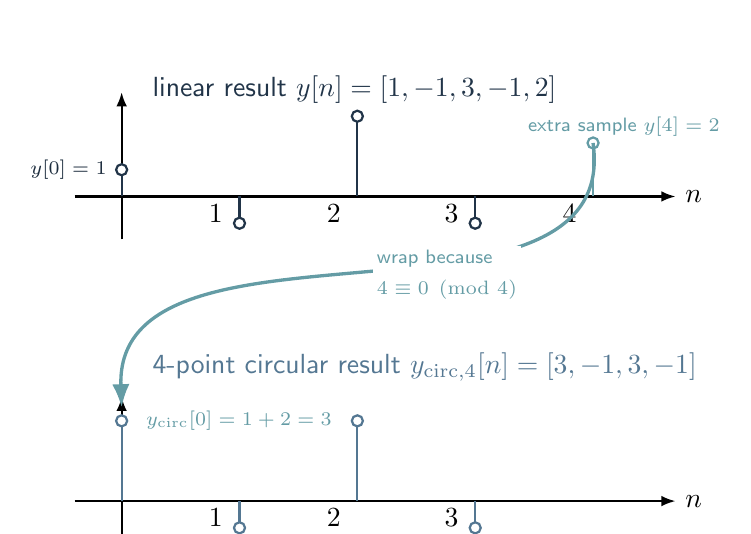
\begin{tikzpicture}[>=Latex]
      \begin{axis}[
          name=wraplinear,
          width=0.76\textwidth, height=3.45cm,
          slideaxis,
          xmin=-0.4, xmax=4.7, ymin=-1.6, ymax=3.9,
          xtick={0,1,2,3,4}, ytick=\empty,
          xticklabel style={xshift=-0.3cm, yshift=0.1cm},
          xlabel={$n$},
          xlabel style={anchor=west}
        ]
        \addplot+[discrete, color=PrimaryColor, mark options={fill=white, draw=PrimaryColor}] coordinates {(0,1) (1,-1) (2,3) (3,-1)};
        \addplot+[discrete, color=AccentColor, mark options={fill=white, draw=AccentColor}] coordinates {(4,2)};
        \node[PrimaryColor, anchor=west] at (axis cs:0.18,4) {linear result \(y[n]=[1,-1,3,-1,2]\)};
        \node[PrimaryColor!85!black, anchor=east, fill=white, inner sep=1pt] at (axis cs:-0.10,1.0) {\scriptsize \(y[0]=1\)};
        \node[AccentColor, anchor=west, fill=white, inner sep=1pt] at (axis cs:3.42,2.62) {\scriptsize extra sample \(y[4]=2\)};
        \coordinate (wrapfrom) at (axis cs:4,2);
      \end{axis}
      \begin{axis}[
          name=wrapcirc,
          at={(wraplinear.south west)}, anchor=north west, yshift=-2cm,
          width=0.76\textwidth, height=3.45cm,
          slideaxis,
          xmin=-0.4, xmax=4.7, ymin=-1.6, ymax=3.9,
          xticklabel style={xshift=-0.3cm, yshift=0.1cm},
          xtick={0,1,2,3}, ytick=\empty,
          xlabel={$n$},
          xlabel style={anchor=west}
        ]
        \addplot+[discrete, color=SecondaryColor, mark options={fill=white, draw=SecondaryColor}] coordinates {(0,3) (1,-1) (2,3) (3,-1)};
        \node[SecondaryColor, anchor=west] at (axis cs:0.18,5) {4-point circular result \(y_{\mathrm{circ},4}[n]=[3,-1,3,-1]\)};
        \node[AccentColor, anchor=west, fill=white, inner sep=1pt] at (axis cs:0.18,3.02) {\scriptsize \(y_{\mathrm{circ}}[0]=1+2=3\)};
        \coordinate (wrapto) at (axis cs:0,3.5);
      \end{axis}
      \draw[->, very thick, AccentColor]
      (wrapfrom) to[out=-82,in=92]
      node[midway, right=2pt, fill=white, inner sep=1.5pt, align=left, text=AccentColor] {\scriptsize wrap because\\[-1pt]\scriptsize \(4\equiv 0 \pmod 4\)}
      (wrapto);
    \end{tikzpicture}
  \end{center}
\end{examplebox}

\section{Nyquist-Shannon Sampling Theorem}

\begin{examplebox}{Problem 5.1}
  \Prompt{State the Nyquist-Shannon sampling theorem in both angular-frequency and ordinary-frequency form.}

  \medskip
  \SketchLabel{}
  If a continuous-time signal is bandlimited to \(|\omega|\le \omega_M\), then exact reconstruction from uniform samples is possible whenever
  \[
    \omega_s>2\omega_M.
  \]
  In ordinary frequency,
  \[
    f_s>2f_M.
  \]
  The sampled spectrum is
  \[
    X_p(j\omega)=\frac{1}{T}\sum_{k=-\infty}^{\infty}X\!\bigl(j(\omega-k\omega_s)\bigr),
  \]
  so the theorem is really a non-overlap condition on these repeated copies.

  \begin{center}
    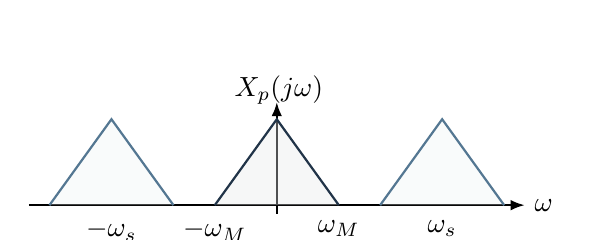
\begin{tikzpicture}
      \begin{axis}[
          width=0.65\textwidth, height=3.0cm,
          slideaxis,
          xmin=-12, xmax=12, ymin=-0.1, ymax=1.2,
          xtick={-3,3,-8,8}, xticklabels={$-\omega_M$,$\omega_M$,$-\omega_s$,$\omega_s$},
          ytick=\empty,
          xlabel={$\omega$},
          xlabel style={anchor=west}
        ]
        \addplot[PrimaryColor, thick, fill=PrimaryColor!12, fill opacity=0.35] coordinates {(-3,0) (0,1) (3,0)};
        \addplot[SecondaryColor, thick, fill=SecondaryColor!12, fill opacity=0.28] coordinates {(5,0) (8,1) (11,0)};
        \addplot[SecondaryColor, thick, fill=SecondaryColor!12, fill opacity=0.28] coordinates {(-11,0) (-8,1) (-5,0)};
        \node[anchor=south] at (axis cs:0.1,1.06) {$X_p(j\omega)$};
      \end{axis}
    \end{tikzpicture}
  \end{center}
\end{examplebox}

\newpage

\begin{examplebox}{Problem 5.2}
  \Prompt{Derive the condition \(\omega_s>2\omega_M\) by comparing adjacent spectral copies of a bandlimited spectrum.}

  \medskip
  \SketchLabel{}
  The sampled spectrum contains copies centered at integer multiples of \(\omega_s\). No overlap requires
  \[
    \omega_s-\omega_M>\omega_M \quad \Longrightarrow \quad \omega_s>2\omega_M.
  \]

  \begin{center}
    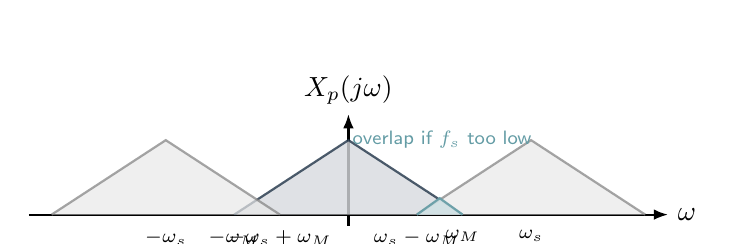
\begin{tikzpicture}
      \begin{axis}[
          width=0.8\textwidth, height=3.0cm,
          slideaxis,
          xmin=-14, xmax=14, ymin=-0.15, ymax=1.35,
          xtick={-8,-5,-3,3,5,8}, xticklabels={$-\omega_s$, $-\omega_M$, $-\omega_s + \omega_M$, $\omega_s-\omega_M$, $\omega_M$, $\omega_s$},
          ytick=\empty,
          xlabel={$\omega$}, ylabel={$X_p(j\omega)$},
          xticklabel style={font=\scriptsize},
          xlabel style={anchor=west}, ylabel style={anchor=south}
        ]
        \addplot[PrimaryColor, thick, fill=PrimaryColor!18, opacity=0.8] coordinates {(-5,0) (0,1) (5,0)};
        \addplot[gray, thick, fill=gray!18, opacity=0.7] coordinates {(3,0) (8,1) (13,0)};
        \addplot[gray, thick, fill=gray!18, opacity=0.7] coordinates {(-13,0) (-8,1) (-3,0)};
        \addplot[AccentColor, thick, fill=AccentColor!30, opacity=0.9] coordinates {(3,0) (4,0.22) (5,0)};
        \node[AccentColor] at (axis cs:4.1,1) {\scriptsize overlap if \(f_s\) too low};
      \end{axis}
    \end{tikzpicture}
  \end{center}
\end{examplebox}

\begin{examplebox}{Problem 5.3}
  \Prompt{A lowpass signal is bandlimited to \(|f|\le 1.6\) kHz. Sketch the sampled spectrum for \(f_s=4.5\) kHz and for \(f_s=2.8\) kHz, and identify which case aliases.}

  \medskip
  \SketchLabel{}
  The Nyquist requirement is
  \[
    f_s>2f_M=3.2\text{ kHz}.
  \]
  So \(f_s=4.5\) kHz is safe, while \(f_s=2.8\) kHz is too low.
  For \(f_s=4.5\) kHz, the central copy occupies \([-1.6,1.6]\) kHz and the nearest shifted copies begin at
  \[
    \pm(4.5-1.6)=\pm 2.9\text{ kHz},
  \]
  leaving a clear gap. For \(f_s=2.8\) kHz, the adjacent copies begin at
  \[
    \pm(2.8-1.6)=\pm 1.2\text{ kHz},
  \]
  which lies inside the central support, so overlap occurs.

  \begin{center}
    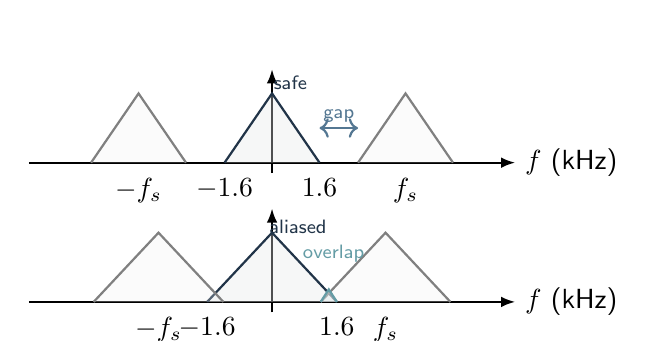
\begin{tikzpicture}
      \begin{axis}[
          name=safealias,
          width=0.64\textwidth, height=2.9cm,
          slideaxis,
          xmin=-8.2, xmax=8.2, ymin=-0.15, ymax=1.35,
          xtick={-4.5,-1.6,1.6,4.5}, xticklabels={$-f_s$,$-1.6$,$1.6$,$f_s$},
          ytick=\empty,
          xlabel={$f$ (kHz)},
          xlabel style={anchor=west}
        ]
        \addplot[PrimaryColor, thick, fill=PrimaryColor!12, fill opacity=0.35] coordinates {(-1.6,0) (0,1) (1.6,0)};
        \addplot[gray, thick, fill=gray!12, fill opacity=0.26] coordinates {(2.9,0) (4.5,1) (6.1,0)};
        \addplot[gray, thick, fill=gray!12, fill opacity=0.26] coordinates {(-6.1,0) (-4.5,1) (-2.9,0)};
        \draw[<->, thick, SecondaryColor] (axis cs:1.6,0.5)--(axis cs:2.9,0.5);
        \node[SecondaryColor] at (axis cs:2.25,0.68) {\scriptsize gap};
        \node[PrimaryColor] at (axis cs:0.62,1.16) {\scriptsize safe};
      \end{axis}
      \begin{axis}[
          at={(safealias.south)}, anchor=north, yshift=-0.45cm,
          width=0.64\textwidth, height=2.9cm,
          slideaxis,
          xmin=-6.0, xmax=6.0, ymin=-0.15, ymax=1.35,
          xtick={-2.8,-1.6,1.6,2.8}, xticklabels={$-f_s$,$-1.6$,$1.6$,$f_s$},
          ytick=\empty,
          xlabel={$f$ (kHz)},
          xlabel style={anchor=west}
        ]
        \addplot[PrimaryColor, thick, fill=PrimaryColor!12, fill opacity=0.35] coordinates {(-1.6,0) (0,1) (1.6,0)};
        \addplot[gray, thick, fill=gray!12, fill opacity=0.26] coordinates {(1.2,0) (2.8,1) (4.4,0)};
        \addplot[gray, thick, fill=gray!12, fill opacity=0.26] coordinates {(-4.4,0) (-2.8,1) (-1.2,0)};
        \addplot[AccentColor, thick, fill=AccentColor!18, fill opacity=0.42] coordinates {(1.2,0) (1.4,0.18) (1.6,0)};
        \node[AccentColor] at (axis cs:1.52,0.7) {\scriptsize overlap};
        \node[PrimaryColor] at (axis cs:0.64,1.08) {\scriptsize aliased};
      \end{axis}
    \end{tikzpicture}
  \end{center}
\end{examplebox}

\begin{examplebox}{Problem 5.4}
  \Prompt{A signal contains tones at \(1.2\) kHz and \(1.8\) kHz. Give one safe sampling frequency and one unsafe sampling frequency.}

  \medskip
  \SketchLabel{}
  Since the highest tone is \(f_M=1.8\) kHz, a safe choice is \(f_s=4\) kHz and an unsafe one is \(f_s=3\) kHz.
  With \(f_s=4\) kHz, the Nyquist frequency is \(2\) kHz, so both tones stay distinct.
  With \(f_s=3\) kHz, the Nyquist frequency is only \(1.5\) kHz, so the \(1.8\) kHz tone folds to
  \[
    f_{\text{alias}}=|1.8-3|=1.2\text{ kHz},
  \]
  colliding with the \(1.2\) kHz tone.

  \begin{center}
    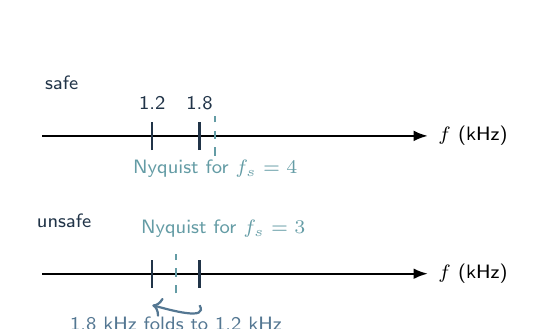
\begin{tikzpicture}[font=\scriptsize]
      \draw[-{Latex[length=1.8mm]}, thick] (-0.2,2.3)--(4.7,2.3) node[right] {$f$ (kHz)};
      \draw[PrimaryColor, thick] (1.2,2.12)--(1.2,2.48);
      \draw[PrimaryColor, thick] (1.8,2.12)--(1.8,2.48);
      \draw[AccentColor, dashed, thick] (2.0,2.05)--(2.0,2.55);
      \node[PrimaryColor] at (1.2,2.72) {1.2};
      \node[PrimaryColor] at (1.8,2.72) {1.8};
      \node[AccentColor] at (2.0,1.88) {Nyquist for \(f_s=4\)};
      \node[PrimaryColor] at (0.05,2.98) {safe};

      \draw[-{Latex[length=1.8mm]}, thick] (-0.2,0.55)--(4.7,0.55) node[right] {$f$ (kHz)};
      \draw[PrimaryColor, thick] (1.2,0.37)--(1.2,0.73);
      \draw[PrimaryColor, thick] (1.8,0.37)--(1.8,0.73);
      \draw[AccentColor, dashed, thick] (1.5,0.3)--(1.5,0.8);
      \draw[->, thick, SecondaryColor] (1.8,0.15) to[out=-60,in=-15] (1.2,0.15);
      \node[AccentColor] at (2.1,1.12) {Nyquist for \(f_s=3\)};
      \node[SecondaryColor] at (1.5,-0.08) {1.8 kHz folds to 1.2 kHz};
      \node[PrimaryColor] at (0.08,1.22) {unsafe};
    \end{tikzpicture}
  \end{center}
\end{examplebox}

\newpage

\section{Ideal Reconstruction, Zero-Order Hold, Linear Interpolation}

\begin{examplebox}{Problem 6.1}
  \Prompt{Write the impulse response and frequency response of the ideal reconstruction filter, and decide whether it is causal.}

  \medskip
  \SketchLabel{}
  The sampled spectrum is
  \[
    X_p(j\omega)=\frac{1}{T}\sum_{r=-\infty}^{\infty}X\!\bigl(j(\omega-r\omega_s)\bigr).
  \]
  To recover the original signal, the ideal filter must keep only the baseband copy in
  \(|\omega|<\omega_s/2\), and it must multiply by \(T\) to cancel the \(1/T\) factor in \(X_p(j\omega)\). Hence
  \[
    H_{\text{ideal}}(j\omega)=
    \begin{cases}
      T,& |\omega|<\omega_s/2,\\
      0,& \text{otherwise},
    \end{cases}
  \]
  The impulse response is the inverse Fourier transform of this rectangle:
  \[
    h_{\text{ideal}}(t)
    =\frac{1}{2\pi}\int_{-\omega_s/2}^{\omega_s/2} T e^{j\omega t}\,d\omega
    =\frac{T}{2\pi}\left[\frac{e^{j\omega t}}{jt}\right]_{-\omega_s/2}^{\omega_s/2}.
  \]
  Therefore
  \[
    h_{\text{ideal}}(t)
    =\frac{T}{\pi t}\sin\!\left(\frac{\omega_s t}{2}\right)
    =\frac{\sin(\pi t/T)}{\pi t/T}
    =\sinc\!\left(\frac{t}{T}\right),
  \]
  because \(\omega_s=2\pi/T\).
  It is noncausal because the sinc extends over both \(t<0\) and \(t>0\).

  \begin{center}
    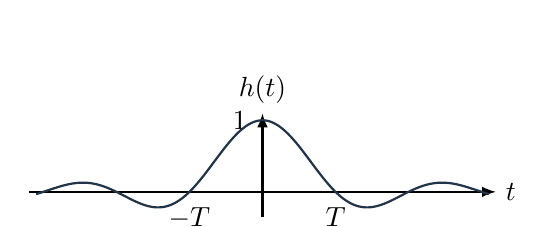
\begin{tikzpicture}
      \begin{axis}[
          width=0.62\textwidth, height=2.9cm,
          slideaxis,
          xmin=-3.2, xmax=3.2, ymin=-0.35, ymax=1.1,
          xtick={-1,1}, xticklabels={$-T$,$T$}, ytick={1},
          xlabel={$t$}, ylabel={$h(t)$},
          xlabel style={anchor=west}, ylabel style={anchor=south}
        ]
        \addplot[signal, domain=-3.1:3.1, samples=200] {abs(x)<0.001 ? 1 : sin(deg(pi*x))/(pi*x)};
      \end{axis}
    \end{tikzpicture}
  \end{center}
\end{examplebox}

\begin{examplebox}{Problem 6.2}
  \Prompt{Derive the impulse response and frequency response of the zero-order hold (ZOH).}

  \medskip
  \SketchLabel{}
  In zero-order hold, one sample \(y(nT)\) is held at full weight until the next sample arrives.
  So the basic reconstruction kernel must be
  \[
    h_0(t)=
    \begin{cases}
      1,& 0\le t<T,\\
      0,& \text{otherwise},
    \end{cases}
    =u(t)-u(t-T).
  \]
  Now take its continuous-time Fourier transform:
  \[
    \begin{aligned}
      H_0(j\omega)
      &=\int_{-\infty}^{\infty} h_0(t)e^{-j\omega t}\,dt
      =\int_0^T e^{-j\omega t}\,dt \\
      &=\left[\frac{e^{-j\omega t}}{-j\omega}\right]_0^T
      =\frac{1-e^{-j\omega T}}{j\omega}.
    \end{aligned}
  \]
  Factor out the midpoint delay:
  \[
    H_0(j\omega)
    =\frac{e^{-j\omega T/2}\bigl(e^{j\omega T/2}-e^{-j\omega T/2}\bigr)}{j\omega}
    =e^{-j\omega T/2}\frac{2\sin(\omega T/2)}{\omega}.
  \]
  Hence
  \[
    H_0(j\omega)=Te^{-j\omega T/2}\sinc\!\left(\frac{\omega T}{2\pi}\right).
  \]
  ZOH is causal because \(h_0(t)=0\) for \(t<0\).

  \begin{center}
    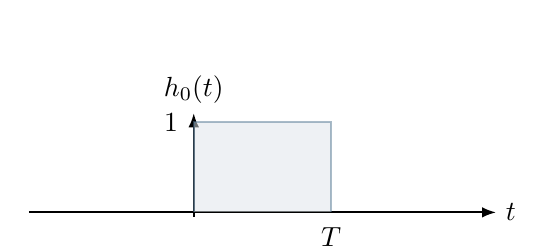
\begin{tikzpicture}
      \begin{axis}[
          width=0.62\textwidth, height=2.9cm,
          slideaxis,
          xmin=-1.2, xmax=2.2, ymin=-0.05, ymax=1.1,
          xtick={0,1}, xticklabels={$0$,$T$}, ytick={1},
          xlabel={$t$}, ylabel={$h_0(t)$},
          xlabel style={anchor=west}, ylabel style={anchor=south}
        ]
        \addplot[SecondaryColor, thick, fill=SecondaryColor!20, opacity=0.5] coordinates {(0,0) (0,1) (1,1) (1,0)};
      \end{axis}
    \end{tikzpicture}
  \end{center}
\end{examplebox}

\newpage

\begin{examplebox}{Problem 6.3}
  \Prompt{Derive the impulse response and frequency response of linear interpolation.}

  \medskip
  \SketchLabel{}
  For linear interpolation, the weight of \(y(nT)\) must rise linearly from \(0\) to \(1\)
  between \((n-1)T\) and \(nT\), then fall linearly from \(1\) to \(0\) between \(nT\) and \((n+1)T\).
  So the basic interpolation kernel is
  \[
    h_1(t)=
    \begin{cases}
      1-|t|/T,& |t|<T,\\
      0,& \text{otherwise},
    \end{cases}.
  \]
  This triangle can also be viewed as the overlap of two centered ZOH rectangles:
  \[
    h_1(t)=\frac{1}{T}\bigl(h_0(t+T/2)*h_0(t+T/2)\bigr).
  \]
  Let \(g(t)=h_0(t+T/2)\). Then \(g(t)\) is a rectangle centered at the origin, so its transform has no linear-phase term:
  \[
    G(j\omega)=\mathcal{F}\{g(t)\}=T\sinc\!\left(\frac{\omega T}{2\pi}\right).
  \]
  By the convolution property,
  \[
    H_1(j\omega)
    =\frac{1}{T}\bigl(G(j\omega)\bigr)^2
    =\frac{1}{T}\left[T\sinc\!\left(\frac{\omega T}{2\pi}\right)\right]^2.
  \]
  Therefore
  \[
    H_1(j\omega)=T\sinc^2\!\left(\frac{\omega T}{2\pi}\right).
  \]
  This symmetric form is noncausal, though a delayed version can be made causal.

  \begin{center}
    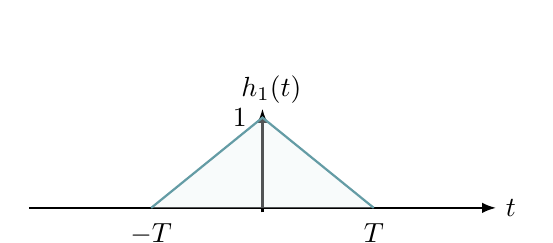
\begin{tikzpicture}
      \begin{axis}[
          width=0.62\textwidth, height=2.9cm,
          slideaxis,
          xmin=-2.1, xmax=2.1, ymin=-0.05, ymax=1.1,
          xtick={-1,1}, xticklabels={$-T$,$T$}, ytick={1},
          xlabel={$t$},
          xlabel style={anchor=west}
        ]
        \addplot[AccentColor, thick, fill=AccentColor!12, fill opacity=0.35] coordinates {(-1,0) (0,1) (1,0)};
        \node[anchor=south] at (axis cs:0.08,1.05) {$h_1(t)$};
      \end{axis}
    \end{tikzpicture}
  \end{center}
\end{examplebox}

\begin{examplebox}{Problem 6.4}
  \Prompt{Compare the magnitude responses of ideal, ZOH, and linear interpolation at \(\omega=\omega_s/4\).}

  \medskip
  \SketchLabel{}
  At \(\omega=\omega_s/4=\pi/(2T)\),
  \[
    \frac{|H_0|}{T}=\sinc\!\left(\frac14\right)=\frac{2\sqrt2}{\pi}\approx0.900,
    \qquad
    \frac{|H_1|}{T}=\sinc^2\!\left(\frac14\right)\approx0.811,
  \]
  while the ideal filter has normalized magnitude \(\frac{|H_{\text{ideal}}|}{T}=1\) (equivalently, \(|H_{\text{ideal}}|=T\)).

  \begin{center}
    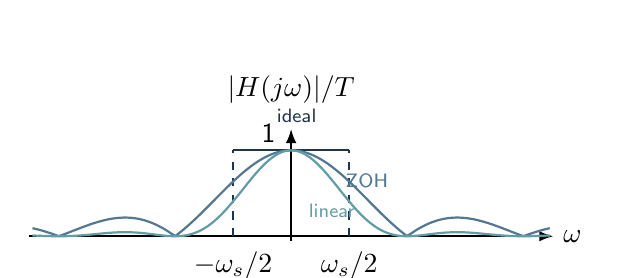
\begin{tikzpicture}
      \begin{axis}[
          width=0.68\textwidth, height=3.0cm,
          slideaxis,
          xmin=-14.2, xmax=14.2, ymin=-0.05, ymax=1.25,
          xtick={-3.14,3.14}, xticklabels={$-\omega_s/2$,$\omega_s/2$},
          ytick={1.2}, yticklabels={1},
          xlabel={$\omega$}, ylabel={$|H(j\omega)|/T$},
          xlabel style={anchor=west}, ylabel style={anchor=south},
          ylabel style={yshift=0.2cm},
          declare function={
            zoh(\x)=abs(\x)<0.001 ? 1 : abs(sin(deg(\x/2))/(\x/2));
            lin(\x)=abs(\x)<0.001 ? 1 : (sin(deg(\x/2))/(\x/2))^2;
          }
        ]
        \addplot[PrimaryColor, thick] coordinates {(-3.14,1) (3.14,1)};
        \draw[PrimaryColor, thick, dashed] (axis cs:-3.14,0)--(axis cs:-3.14,1);
        \draw[PrimaryColor, thick, dashed] (axis cs:3.14,0)--(axis cs:3.14,1);
        \addplot[SecondaryColor, thick, domain=-14:14, samples=200] {zoh(x)};
        \addplot[AccentColor, thick, domain=-14:14, samples=200] {lin(x)};
        \node[PrimaryColor] at (axis cs:0.3,1.4) {\scriptsize ideal};
        \node[SecondaryColor] at (axis cs:4.1,0.65) {\scriptsize ZOH};
        \node[AccentColor] at (axis cs:2.2,0.3) {\scriptsize linear};
      \end{axis}
    \end{tikzpicture}
  \end{center}
\end{examplebox}

\begin{examplebox}{Problem 6.5}
  \Prompt{State one main advantage and one main drawback of each of the three reconstruction methods.}

  \medskip
  \SketchLabel{}
  Ideal reconstruction is perfect in theory but unrealizable in real time. ZOH is extremely easy to implement, but it introduces staircase distortion and sinc droop. Linear interpolation is smoother than ZOH and gives better high-frequency behavior, but it is still not ideal.

  \begin{center}
    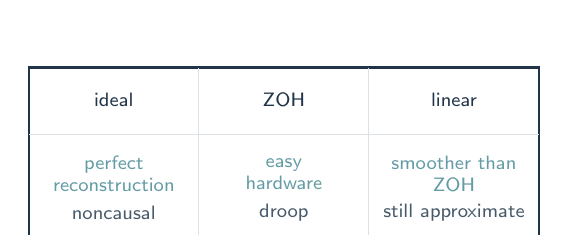
\begin{tikzpicture}[scale=0.9, font=\scriptsize]
      \draw[PrimaryColor, thick] (0,0) rectangle (7.2,2.5);
      \draw[LightGray] (2.4,0)--(2.4,2.5);
      \draw[LightGray] (4.8,0)--(4.8,2.5);
      \draw[LightGray] (0,1.55)--(7.2,1.55);
      \node[PrimaryColor] at (1.2,2.05) {ideal};
      \node[PrimaryColor] at (3.6,2.05) {ZOH};
      \node[PrimaryColor] at (6.0,2.05) {linear};
      \node[AccentColor, align=center] at (1.2,1.0) {perfect\\reconstruction};
      \node[AccentColor, align=center] at (3.6,1.0) {easy\\hardware};
      \node[AccentColor, align=center] at (6.0,1.0) {smoother than\\ZOH};
      \node[DarkGray] at (1.2,0.45) {noncausal};
      \node[DarkGray] at (3.6,0.45) {droop};
      \node[DarkGray] at (6.0,0.45) {still approximate};
    \end{tikzpicture}
  \end{center}
\end{examplebox}

\newpage

\section{Laplace Transform: Definition, Properties, ROC, Poles and Zeros}

\begin{examplebox}{Problem 7.1}
  \Prompt{Find the Laplace transform and ROC of \(x(t)=(t-2)e^{-3(t-2)}u(t-2)\).}

  \medskip
  \SketchLabel{}
  \[
    \Lpair{e^{-3t}u(t)}{\frac{1}{s+3}},
    \qquad
    \ROC:\ \text{Re}\{s\}>-3.
  \]
  \[
    \Lpair{t e^{-3t}u(t)}{\frac{1}{(s+3)^2}},
    \qquad
    \ROC:\ \text{Re}\{s\}>-3.
  \]
  Applying the time-shift property to delay the signal by \(2\),
  \[
    \Lpair{(t-2)e^{-3(t-2)}u(t-2)}{e^{-2s}\dfrac{1}{(s+3)^2}},
    \qquad
    \ROC:\ \text{Re}\{s\}>-3.
  \]

  \begin{center}
    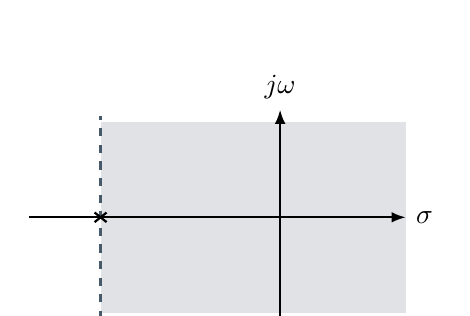
\begin{tikzpicture}[scale=0.76]
      \fill[PrimaryColor, fill opacity=0.14] (-3,-1.6) rectangle (2.1,1.6);
      \draw[-{Latex[length=1.8mm]}, thick] (-4.2,0)--(2.1,0) node[right] {$\sigma$};
      \draw[-{Latex[length=1.8mm]}, thick] (0,-1.8)--(0,1.8) node[above] {$j\omega$};
      \draw[dashed, thick, DarkGray] (-3,-1.7)--(-3,1.7);
      \draw[thick] (-3.1,0.08)--(-2.9,-0.08);
      \draw[thick] (-3.1,-0.08)--(-2.9,0.08);
    \end{tikzpicture}
  \end{center}
\end{examplebox}

\begin{examplebox}{Problem 7.2}
  \Prompt{Find the Laplace transform and ROC of \(x(t)=t^2 e^{-3t}u(t)\).}

  \medskip
  \SketchLabel{}
  Start from
  \[
    \Lpair{e^{-3t}u(t)}{\frac{1}{s+3}},
    \qquad
    \ROC:\ \text{Re}\{s\}>-3.
  \]
  Differentiate once in the \(s\)-domain:
  \[
    \Lpair{te^{-3t}u(t)}{-\frac{d}{ds}\!\left(\frac{1}{s+3}\right)
    =\frac{1}{(s+3)^2}},
    \qquad
    \ROC:\ \text{Re}\{s\}>-3.
  \]
  Differentiate once more:
  \[
    \Lpair{t^2 e^{-3t}u(t)}{-\frac{d}{ds}\!\left(\frac{1}{(s+3)^2}\right)
    =\frac{2}{(s+3)^3}},
    \qquad
    \ROC:\ \text{Re}\{s\}>-3.
  \]

  \begin{center}
    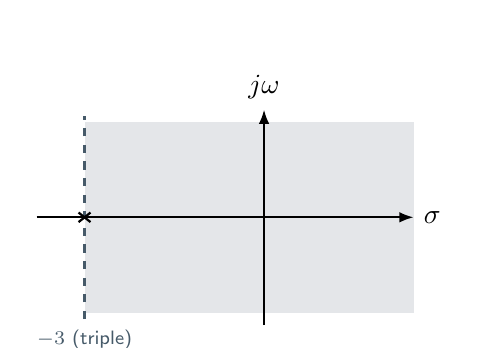
\begin{tikzpicture}[scale=0.76]
      \fill[PrimaryColor, fill opacity=0.12] (-3,-1.6) rectangle (2.5,1.6);
      \draw[-{Latex[length=1.8mm]}, thick] (-3.8,0)--(2.5,0) node[right] {$\sigma$};
      \draw[-{Latex[length=1.8mm]}, thick] (0,-1.8)--(0,1.8) node[above] {$j\omega$};
      \draw[dashed, thick, DarkGray] (-3,-1.7)--(-3,1.7);
      \draw[thick] (-3.1,0.08)--(-2.9,-0.08); \draw[thick] (-3.1,-0.08)--(-2.9,0.08);
      \node[DarkGray] at (-3,-2.05) {\scriptsize $-3$ (triple)};
    \end{tikzpicture}
  \end{center}
\end{examplebox}

\begin{examplebox}{Problem 7.3}
  \Prompt{Find the Laplace transform and ROC of \(x(t)=t e^{-t}u(t)+e^{2t}u(-t)\).}

  \medskip
  \SketchLabel{}
  \[
    \Lpair{e^{-t}u(t)}{\frac{1}{s+1}},
    \qquad
    \ROC:\ \text{Re}\{s\}>-1.
  \]
  Hence
  \[
    \Lpair{t e^{-t}u(t)}{-\frac{d}{ds}\!\left(\frac{1}{s+1}\right)
    =\frac{1}{(s+1)^2}},
    \qquad
    \ROC:\ \text{Re}\{s\}>-1.
  \]
  For the left-sided term,
  \[
    \Lpair{e^{2t}u(-t)}{-\frac{1}{s-2}},
    \qquad
    \ROC:\ \text{Re}\{s\}<2.
  \]
  Therefore
  \[
    X(s)=\frac{1}{(s+1)^2}-\frac{1}{s-2},
    \qquad
    \ROC:\ -1<\text{Re}\{s\}<2.
  \]

  \begin{center}
    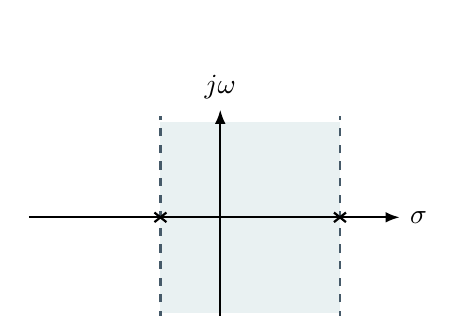
\begin{tikzpicture}[scale=0.76]
      \fill[AccentColor, fill opacity=0.14] (-1,-1.6) rectangle (2,1.6);
      \draw[-{Latex[length=1.8mm]}, thick] (-3.2,0)--(3.0,0) node[right] {$\sigma$};
      \draw[-{Latex[length=1.8mm]}, thick] (0,-1.8)--(0,1.8) node[above] {$j\omega$};
      \draw[dashed, thick, DarkGray] (-1,-1.7)--(-1,1.7);
      \draw[dashed, thick, DarkGray] (2,-1.7)--(2,1.7);
      \draw[thick] (-1.1,0.08)--(-0.9,-0.08);
      \draw[thick] (-1.1,-0.08)--(-0.9,0.08);
      \draw[thick] (1.9,0.08)--(2.1,-0.08);
      \draw[thick] (1.9,-0.08)--(2.1,0.08);
    \end{tikzpicture}
  \end{center}
\end{examplebox}

\begin{examplebox}{Problem 7.4}
  \Prompt{Find the Laplace transform and ROC of \(x(t)=e^{-4(t-1)}\cos\!\bigl(3(t-1)\bigr)u(t-1)\).}

  \medskip
  \SketchLabel{}
  \[
    e^{-4t}\cos(3t)u(t)
    =\frac{1}{2}\Bigl(e^{(-4+3j)t}+e^{(-4-3j)t}\Bigr)u(t).
  \]
  \[
    \Lpair{e^{(-4+3j)t}u(t)}{\frac{1}{s+4-3j}},
    \Lpair{e^{(-4-3j)t}u(t)}{\frac{1}{s+4+3j}},
    \qquad
    \ROC:\ \text{Re}\{s\}>-4.
  \]
  Therefore
  \[
    \Lpair{e^{-4t}\cos(3t)u(t)}
    {\frac{1}{2}\left(\frac{1}{s+4-3j}+\frac{1}{s+4+3j}\right)
    =\frac{s+4}{(s+4)^2+9}},
    \qquad
    \ROC:\ \text{Re}\{s\}>-4.
  \]
  Applying a delay of \(1\) multiplies the transform by \(e^{-s}\) without changing the ROC:
  \[
    \Lpair{e^{-4(t-1)}\cos\!\bigl(3(t-1)\bigr)u(t-1)}
    {e^{-s}\dfrac{s+4}{(s+4)^2+9}},
    \qquad
    \ROC:\ \text{Re}\{s\}>-4.
  \]

  \begin{center}
    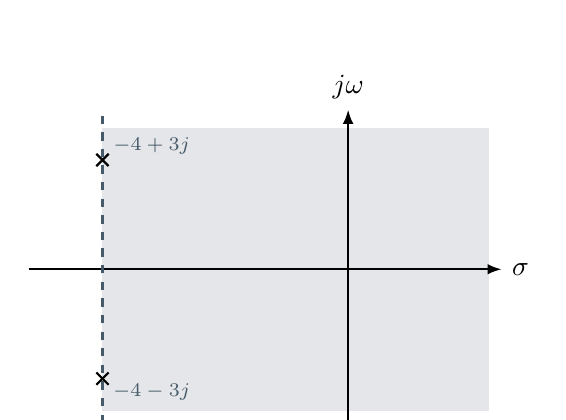
\begin{tikzpicture}[scale=0.78]
      \fill[PrimaryColor, fill opacity=0.12] (-4,-2.3) rectangle (2.3,2.3);
      \draw[-{Latex[length=1.8mm]}, thick] (-5.2,0)--(2.5,0) node[right] {$\sigma$};
      \draw[-{Latex[length=1.8mm]}, thick] (0,-2.6)--(0,2.6) node[above] {$j\omega$};
      \draw[dashed, thick, DarkGray] (-4,-2.5)--(-4,2.5);
      \draw[thick] (-4.1,1.68)--(-3.9,1.88); \draw[thick] (-4.1,1.88)--(-3.9,1.68);
      \draw[thick] (-4.1,-1.68)--(-3.9,-1.88); \draw[thick] (-4.1,-1.88)--(-3.9,-1.68);
      \node[DarkGray] at (-3.2,2.0) {\scriptsize $-4+3j$};
      \node[DarkGray] at (-3.2,-2.0) {\scriptsize $-4-3j$};
    \end{tikzpicture}
  \end{center}
\end{examplebox}

\begin{examplebox}{Problem 7.5}
  \Prompt{Find the Laplace transform, ROC, poles, and zeros of \(x(t)=t e^{-t}\sin(2t)u(t)\).}

  \medskip
  \SketchLabel{}
  \[
    e^{-t}\sin(2t)u(t)
    =\frac{1}{2j}\Bigl(e^{(-1+2j)t}-e^{(-1-2j)t}\Bigr)u(t).
  \]
  \[
    \Lpair{e^{(-1+2j)t}u(t)}{\frac{1}{s+1-2j}},
    \Lpair{e^{(-1-2j)t}u(t)}{\frac{1}{s+1+2j}},
    \qquad
    \ROC:\ \text{Re}\{s\}>-1.
  \]
  Therefore
  \[
    \Lpair{e^{-t}\sin(2t)u(t)}
    {\frac{1}{2j}\left(\frac{1}{s+1-2j}-\frac{1}{s+1+2j}\right)
    =\frac{2}{(s+1)^2+4}},
    \qquad
    \ROC:\ \text{Re}\{s\}>-1.
  \]
  Differentiate in the \(s\)-domain:
  \[
    \Lpair{t e^{-t}\sin(2t)u(t)}{-\frac{d}{ds}\!\left(\frac{2}{(s+1)^2+4}\right)
    =\frac{4(s+1)}{\bigl((s+1)^2+4\bigr)^2}},
    \qquad
    \ROC:\ \text{Re}\{s\}>-1.
  \]
  The poles are double poles at \(s=-1\pm2j\), and the finite zero is at \(s=-1\).

  \begin{center}
    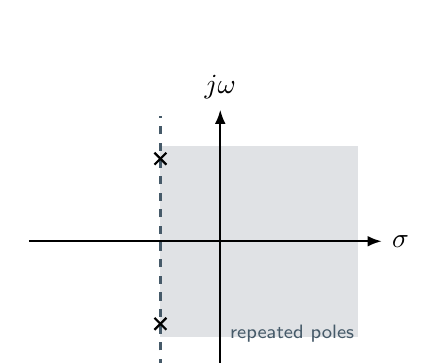
\begin{tikzpicture}[scale=0.76]
      \fill[PrimaryColor, fill opacity=0.14] (-1,-1.6) rectangle (2.3,1.6);
      \draw[-{Latex[length=1.8mm]}, thick] (-3.2,0)--(2.7,0) node[right] {$\sigma$};
      \draw[-{Latex[length=1.8mm]}, thick] (0,-2.2)--(0,2.2) node[above] {$j\omega$};
      \draw[dashed, thick, DarkGray] (-1,-2.1)--(-1,2.1);
      \draw[thick] (-1.1,1.48)--(-0.9,1.28);
      \draw[thick] (-1.1,1.28)--(-0.9,1.48);
      \draw[thick] (-1.1,-1.28)--(-0.9,-1.48);
      \draw[thick] (-1.1,-1.48)--(-0.9,-1.28);
      \node[DarkGray] at (1.2,-1.55) {\scriptsize repeated poles};
    \end{tikzpicture}
  \end{center}
\end{examplebox}

\begin{examplebox}{Problem 7.6}
  \Prompt{Find the Laplace transform and ROC of \(y(t)=\bigl(e^{-t}\sin(3t)\,u(t)\bigr)*\bigl(e^{-2t}u(t)\bigr)\).}

  \medskip
  \SketchLabel{}
  \[
    e^{-t}\sin(3t)u(t)
    =\frac{1}{2j}\Bigl(e^{(-1+3j)t}-e^{(-1-3j)t}\Bigr)u(t).
  \]
  \[
    \Lpair{e^{(-1+3j)t}u(t)}{\frac{1}{s+1-3j}},
    \Lpair{e^{(-1-3j)t}u(t)}{\frac{1}{s+1+3j}},
    \qquad
    \ROC:\ \text{Re}\{s\}>-1.
  \]
  Hence
  \[
    \Lpair{e^{-t}\sin(3t)\,u(t)}
    {\frac{1}{2j}\left(\frac{1}{s+1-3j}-\frac{1}{s+1+3j}\right)
    =\frac{3}{(s+1)^2+9}},
    \qquad
    \ROC:\ \text{Re}\{s\}>-1.
  \]
  Also
  \[
    \Lpair{e^{-2t}u(t)}{\frac{1}{s+2}},
    \qquad
    \ROC:\ \text{Re}\{s\}>-2.
  \]
  By the \textbf{convolution property}, convolution in time becomes multiplication in the \(s\)-domain, so
  \[
    Y(s)=\frac{3}{((s+1)^2+9)(s+2)},
    \qquad
    \ROC:\ \text{Re}\{s\}>-1\;\;\text{(intersection)}.
  \]
  Poles: \(s=-1\pm 3j\) and \(s=-2\). No finite zeros.

  \begin{center}
    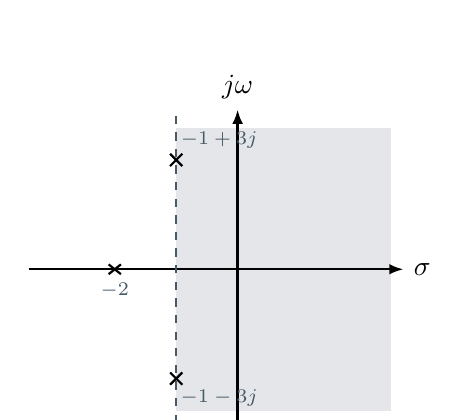
\begin{tikzpicture}[scale=0.78]
      \fill[PrimaryColor, fill opacity=0.12] (-1,-2.3) rectangle (2.5,2.3);
      \draw[-{Latex[length=1.8mm]}, thick] (-3.4,0)--(2.7,0) node[right] {$\sigma$};
      \draw[-{Latex[length=1.8mm]}, thick] (0,-2.6)--(0,2.6) node[above] {$j\omega$};
      \draw[dashed, thick, DarkGray] (-1,-2.5)--(-1,2.5);
      % poles
      \draw[thick] (-1.1,1.88)--(-0.9,1.68); \draw[thick] (-1.1,1.68)--(-0.9,1.88);
      \draw[thick] (-1.1,-1.68)--(-0.9,-1.88); \draw[thick] (-1.1,-1.88)--(-0.9,-1.68);
      \draw[thick] (-2.1,0.08)--(-1.9,-0.08); \draw[thick] (-2.1,-0.08)--(-1.9,0.08);
      \node[DarkGray] at (-0.3,2.1) {\scriptsize $-1+3j$};
      \node[DarkGray] at (-0.3,-2.1) {\scriptsize $-1-3j$};
      \node[DarkGray] at (-2,-0.35) {\scriptsize $-2$};
    \end{tikzpicture}
  \end{center}
\end{examplebox}

\vfill

\begin{conceptbox}{Residue Method for Partial Fractions}
  For rational transforms, partial-fraction coefficients can be obtained directly using residue formulas (same idea you saw from Laurent-series coefficients; no extra complex-analysis machinery needed here).

  Let
  \[
    F(s)=\frac{P(s)}{Q(s)}.
  \]

  For a \textbf{simple pole} at \(s=p\):
  \[
    F(s)=\frac{A}{s-p}+\cdots,
    \qquad
    A=\operatorname*{Res}_{s=p}F(s)=\lim_{s\to p}(s-p)F(s).
  \]

  For a \textbf{double pole} at \(s=p\):
  \[
    F(s)=\frac{A_2}{(s-p)^2}+\frac{A_1}{s-p}+\cdots,
  \]
  \[
    A_2=\lim_{s\to p}(s-p)^2F(s),
    \qquad
    A_1=\left.\frac{d}{ds}\Big((s-p)^2F(s)\Big)\right|_{s=p}.
  \]

  For a pole of \textbf{order \(m\)} at \(s=p\):
  \[
    F(s)=\frac{A_m}{(s-p)^m}+\frac{A_{m-1}}{(s-p)^{m-1}}+\cdots+\frac{A_1}{s-p}+\cdots,
    \qquad
    A_k=\frac{1}{(m-k)!}\left.\frac{d^{\,m-k}}{ds^{\,m-k}}\Big((s-p)^mF(s)\Big)\right|_{s=p}.
  \]

  These derivatives can be easily computed using a calculator. The same formulas work in the \(z\)-transform section by setting \(r=z^{-1}\), turning factors into \((1-ar)\).
\end{conceptbox}

\newpage

\section{Inverse Laplace Transform}

\begin{examplebox}{Problem 8.1}
  \Prompt{Invert \(X(s)=\dfrac{3s+7}{(s+1)(s+2)}\) with ROC \(\text{Re}\{s\}>-1\).}

  \medskip
  \SketchLabel{}
  Partial-fraction expansion:
  \[
    \frac{3s+7}{(s+1)(s+2)}=\frac{A}{s+1}+\frac{B}{s+2}.
  \]
  Using residues at the simple poles,
  \[
    A=\lim_{s\to-1}(s+1)\frac{3s+7}{(s+1)(s+2)}=4,
    \qquad
    B=\lim_{s\to-2}(s+2)\frac{3s+7}{(s+1)(s+2)}=-1.
  \]
  Since the ROC is to the right of both poles, both terms are right-sided:
  \[
    x(t)=\bigl(4e^{-t}-e^{-2t}\bigr)u(t).
  \]

  \begin{center}
    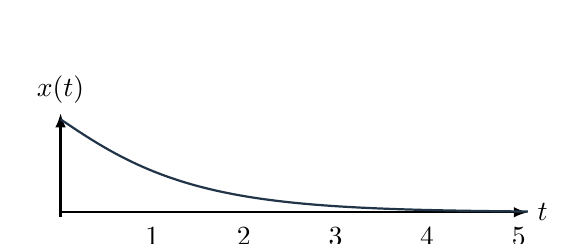
\begin{tikzpicture}
      \begin{axis}[
          width=0.62\textwidth, height=2.9cm,
          slideaxis,
          xmin=0, xmax=5.1, ymin=-0.15, ymax=3.2,
          xtick={0,1,2,3,4,5}, ytick=\empty,
          xlabel={$t$}, ylabel={$x(t)$},
          xlabel style={anchor=west}, ylabel style={anchor=south}
        ]
        \addplot[signal, domain=0:5.1, samples=180] {4*exp(-x)-exp(-2*x)};
      \end{axis}
    \end{tikzpicture}
  \end{center}
\end{examplebox}

\begin{examplebox}{Problem 8.2}
  \Prompt{Invert \(X(s)=\dfrac{2s+3}{s^2+2s+5}\) with ROC \(\text{Re}\{s\}>-1\).}

  \medskip
  \SketchLabel{}
  If one remembers the standard pair for \(e^{at}\sin(bt)\), this inversion becomes much shorter. Here we derive it directly from the complex poles instead of assuming that pair.
  First factor the denominator over the complex numbers:
  \[
    s^2+2s+5=(s+1)^2+4=(s+1-2j)(s+1+2j).
  \]
  So write
  \[
    X(s)=\frac{A}{s+1-2j}+\frac{B}{s+1+2j},
    \qquad
    \ROC:\ \text{Re}\{s\}>-1.
  \]
  Using residues at the two simple poles,
  \[
    A=\lim_{s\to -1+2j}(s+1-2j)X(s)
    =\frac{2(-1+2j)+3}{(-1+2j)+1+2j}
    =\frac{1+4j}{4j}
    =1-\frac{j}{4},
  \]
  \[
    B=\lim_{s\to -1-2j}(s+1+2j)X(s)
    =\frac{2(-1-2j)+3}{(-1-2j)+1-2j}
    =\frac{1-4j}{-4j}
    =1+\frac{j}{4}.
  \]
  Therefore
  \[
    X(s)=\frac{1-\frac{j}{4}}{s+1-2j}+\frac{1+\frac{j}{4}}{s+1+2j},
    \qquad
    \ROC:\ \text{Re}\{s\}>-1.
  \]
  Since the ROC is to the right of both poles, both terms are right-sided:
  \[
    \Linvpair{\frac{1}{s+1-2j}}{e^{(-1+2j)t}u(t)},
    \qquad
    \Linvpair{\frac{1}{s+1+2j}}{e^{(-1-2j)t}u(t)},
    \qquad
    \ROC:\ \text{Re}\{s\}>-1.
  \]
  Hence
  \[
    x(t)=\left(1-\frac{j}{4}\right)e^{(-1+2j)t}u(t)
    +\left(1+\frac{j}{4}\right)e^{(-1-2j)t}u(t).
  \]
  Factor out \(e^{-t}u(t)\):
  \[
    x(t)=e^{-t}\left[\left(1-\frac{j}{4}\right)e^{j2t}
    +\left(1+\frac{j}{4}\right)e^{-j2t}\right]u(t).
  \]
  Now combine the conjugate terms:
  \[
    \left(1-\frac{j}{4}\right)e^{j2t}
    +\left(1+\frac{j}{4}\right)e^{-j2t}
    =(e^{j2t}+e^{-j2t})+\frac{j}{4}(e^{-j2t}-e^{j2t}).
  \]
  Using Euler's identities
  \[
    e^{j2t}+e^{-j2t}=2\cos 2t,
    \qquad
    e^{-j2t}-e^{j2t}=-2j\sin 2t,
  \]
  we get
  \[
    x(t)=\left(2e^{-t}\cos 2t+\tfrac{1}{2}e^{-t}\sin 2t\right)u(t).
  \]

  \begin{center}
    \begin{minipage}{0.42\textwidth}\centering
      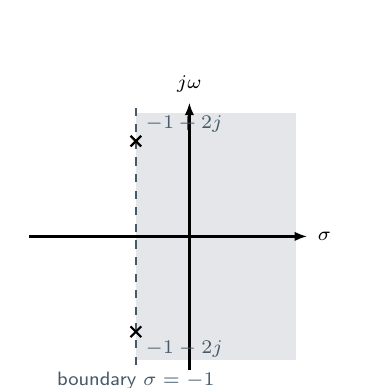
\begin{tikzpicture}[scale=0.68]
        \fill[PrimaryColor, fill opacity=0.12] (-1,-2.3) rectangle (2.0,2.3);
        \draw[-{Latex[length=1.6mm]}, thick] (-3.0,0)--(2.2,0) node[right] {\scriptsize$\sigma$};
        \draw[-{Latex[length=1.6mm]}, thick] (0,-2.5)--(0,2.5) node[above] {\scriptsize$j\omega$};
        \draw[dashed, thick, DarkGray] (-1,-2.4)--(-1,2.4);
        \draw[thick] (-1.1,1.88)--(-0.9,1.68); \draw[thick] (-1.1,1.68)--(-0.9,1.88);
        \draw[thick] (-1.1,-1.68)--(-0.9,-1.88); \draw[thick] (-1.1,-1.88)--(-0.9,-1.68);
        \node[DarkGray] at (-0.1,2.1) {\scriptsize $-1+2j$};
        \node[DarkGray] at (-0.1,-2.1) {\scriptsize $-1-2j$};
        \node[DarkGray] at (-1,-2.7) {\scriptsize boundary $\sigma=-1$};
      \end{tikzpicture}
    \end{minipage}\hfill
    \begin{minipage}{0.55\textwidth}\centering
      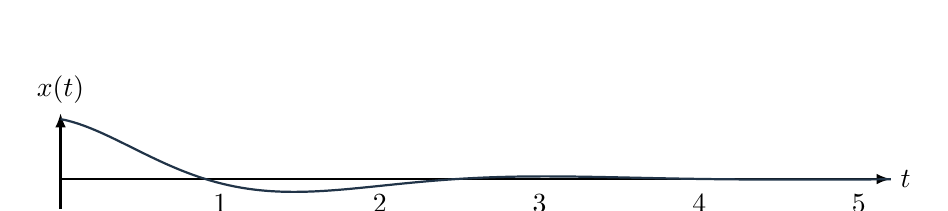
\begin{tikzpicture}
        \begin{axis}[
            width=\textwidth, height=2.8cm,
            slideaxis,
            xmin=0, xmax=5.2, ymin=-1.0, ymax=2.2,
            xtick={0,1,2,3,4,5}, ytick=\empty,
            xlabel={$t$}, ylabel={$x(t)$},
            xlabel style={anchor=west}, ylabel style={anchor=south}
          ]
          \addplot[signal, domain=0:5.2, samples=220] {exp(-x)*(2*cos(deg(2*x))+0.5*sin(deg(2*x)))};
        \end{axis}
      \end{tikzpicture}
    \end{minipage}
  \end{center}
\end{examplebox}

\begin{examplebox}{Problem 8.3}
  \Prompt{Invert \(X(s)=\dfrac{-5}{(s+1)(s-4)}\) with ROC \(-1<\text{Re}\{s\}<4\).}

  \medskip
  \SketchLabel{}
  Partial fractions:
  \[
    \frac{-5}{(s+1)(s-4)}=\frac{1}{s+1}-\frac{1}{s-4}.
  \]
  Coefficients from simple-pole residues:
  \[
    \lim_{s\to-1}(s+1)\frac{-5}{(s+1)(s-4)}=1,
    \qquad
    \lim_{s\to4}(s-4)\frac{-5}{(s+1)(s-4)}=-1.
  \]
  The ROC is a \emph{strip} between the two poles, so we need a two-sided signal:
  \begin{itemize}
    \item Pole at \(s=-1\): to the left of the strip \(\Rightarrow\) right-sided term \(e^{-t}u(t)\).
    \item Pole at \(s=4\): to the right of the strip \(\Rightarrow\) left-sided term. Since
      \(\Linvpair{\frac{1}{s-4}}{-e^{4t}u(-t)}\) for \(\text{Re}\{s\}<4\), the second term gives \(e^{4t}u(-t)\).
  \end{itemize}
  \[
    x(t)=e^{-t}u(t)+e^{4t}u(-t).
  \]

  \begin{center}
    \begin{minipage}{0.42\textwidth}\centering
      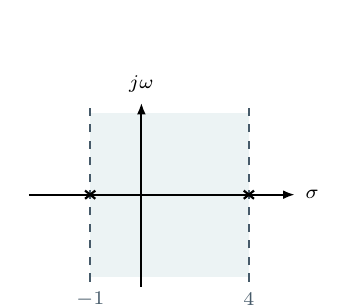
\begin{tikzpicture}[scale=0.65]
        \fill[AccentColor, fill opacity=0.12] (-1,-1.6) rectangle (2.1,1.6);
        \draw[-{Latex[length=1.5mm]}, thick] (-2.2,0)--(3.0,0) node[right] {\scriptsize$\sigma$};
        \draw[-{Latex[length=1.5mm]}, thick] (0,-1.8)--(0,1.8) node[above] {\scriptsize$j\omega$};
        \draw[dashed, thick, DarkGray] (-1,-1.7)--(-1,1.7);
        \draw[dashed, thick, DarkGray] (2.1,-1.7)--(2.1,1.7);
        \draw[thick] (-1.1,0.08)--(-0.9,-0.08); \draw[thick] (-1.1,-0.08)--(-0.9,0.08);
        \draw[thick] (2.0,0.08)--(2.2,-0.08); \draw[thick] (2.0,-0.08)--(2.2,0.08);
        \node[DarkGray] at (-1,-2.05) {\scriptsize $-1$};
        \node[DarkGray] at (2.1,-2.05) {\scriptsize $4$};
      \end{tikzpicture}
    \end{minipage}\hfill
    \begin{minipage}{0.55\textwidth}\centering
      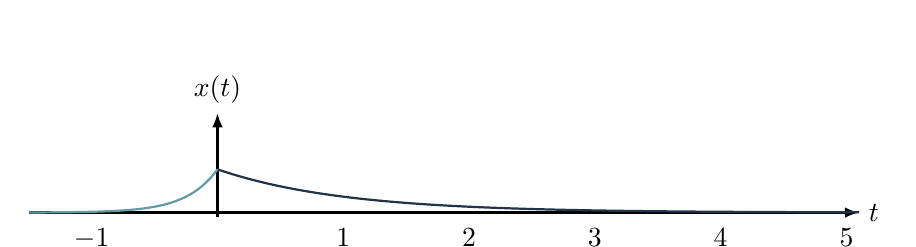
\begin{tikzpicture}
        \begin{axis}[
            width=\textwidth, height=2.9cm,
            slideaxis,
            xmin=-1.5, xmax=5.1, ymin=-0.1, ymax=2.3,
            xtick={-1,0,1,2,3,4,5}, ytick=\empty,
            xlabel={$t$}, ylabel={$x(t)$},
            xlabel style={anchor=west}, ylabel style={anchor=south}
          ]
          \addplot[signal, domain=0:5.1, samples=120] {exp(-x)};
          \addplot[AccentColor, thick, domain=-1.5:0, samples=120] {exp(4*x)};
        \end{axis}
      \end{tikzpicture}
    \end{minipage}
  \end{center}
\end{examplebox}

\begin{examplebox}{Problem 8.4}
  \Prompt{Invert \(X(s)=\dfrac{s}{(s^2+4)^2}\) with ROC \(\text{Re}\{s\}>0\).}

  \medskip
  \SketchLabel{}
  One can also decompose this into repeated complex poles at \(s=\pm 2j\) and invert by partial fractions, but recognizing the sine pair followed by the derivative method is more direct.
  \[
    \Linvpair{\frac{2}{s^2+4}}{\sin(2t)u(t)},
    \qquad
    \ROC:\ \text{Re}\{s\}>0.
  \]
  Using \(\Linvpair{-\dfrac{dX}{ds}}{t\,x(t)}\),
  \[
    -\frac{d}{ds}\!\left(\frac{2}{s^2+4}\right)=\frac{4s}{(s^2+4)^2},
    \qquad
    \ROC:\ \text{Re}\{s\}>0,
  \]
  so
  \[
    \Linvpair{\frac{4s}{(s^2+4)^2}}{t\sin(2t)u(t)},
    \qquad
    \ROC:\ \text{Re}\{s\}>0.
  \]
  Therefore
  \[
    x(t)=\frac14\,t\sin(2t)u(t),
    \qquad
    \ROC:\ \text{Re}\{s\}>0.
  \]

  \begin{center}
    \begin{minipage}{0.42\textwidth}\centering
      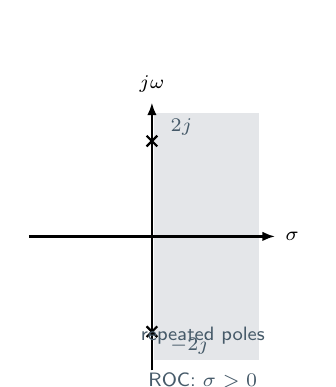
\begin{tikzpicture}[scale=0.68]
        \fill[PrimaryColor, fill opacity=0.12] (0.03,-2.3) rectangle (2.0,2.3);
        \draw[-{Latex[length=1.6mm]}, thick] (-2.3,0)--(2.3,0) node[right] {\scriptsize$\sigma$};
        \draw[-{Latex[length=1.6mm]}, thick] (0,-2.5)--(0,2.5) node[above] {\scriptsize$j\omega$};
        \draw[thick] (-0.1,1.88)--(0.1,1.68); \draw[thick] (-0.1,1.68)--(0.1,1.88);
        \draw[thick] (-0.1,-1.68)--(0.1,-1.88); \draw[thick] (-0.1,-1.88)--(0.1,-1.68);
        \node[DarkGray] at (0.55,2.05) {\scriptsize $2j$};
        \node[DarkGray] at (0.7,-2.05) {\scriptsize $-2j$};
        \node[DarkGray] at (0.95,-2.7) {\scriptsize ROC: $\sigma>0$};
        \node[DarkGray] at (0.95,-1.85) {\scriptsize repeated poles};
      \end{tikzpicture}
    \end{minipage}\hfill
    \begin{minipage}{0.55\textwidth}\centering
      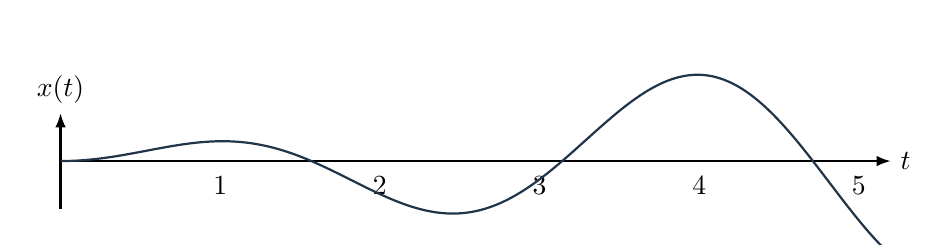
\begin{tikzpicture}
        \begin{axis}[
            width=\textwidth, height=2.8cm,
            slideaxis,
            xmin=0, xmax=5.2, ymin=-0.55, ymax=0.55,
            xtick={0,1,2,3,4,5}, ytick=\empty,
            xlabel={$t$}, ylabel={$x(t)$},
            xlabel style={anchor=west}, ylabel style={anchor=south}
          ]
          \addplot[signal, domain=0:5.2, samples=220] {0.25*x*sin(deg(2*x))};
        \end{axis}
      \end{tikzpicture}
    \end{minipage}
  \end{center}
\end{examplebox}

\begin{examplebox}{Problem 8.5}
  \Prompt{Invert \(X(s)=\dfrac{e^{-s}}{s(s+2)}\) with ROC \(\text{Re}\{s\}>0\).}

  \medskip
  \SketchLabel{}
  First ignore the delay factor and define
  \[
    Y(s)=\frac{1}{s(s+2)},
    \qquad
    \ROC:\ \text{Re}\{s\}>0.
  \]
  Partial fractions give
  \[
    \frac{1}{s(s+2)}=\frac{A}{s}+\frac{B}{s+2},
    \qquad
    A=\lim_{s\to0}sY(s)=\frac12,
    \qquad
    B=\lim_{s\to-2}(s+2)Y(s)=-\frac12,
  \]
  so
  \[
    Y(s)=\frac{1/2}{s}-\frac{1/2}{s+2},
    \qquad
    \ROC:\ \text{Re}\{s\}>0.
  \]
  Now invert term by term:
  \[
    \Linvpair{\frac{1/2}{s}}{\frac12\,u(t)},
    \qquad
    \ROC:\ \text{Re}\{s\}>0,
  \]
  \[
    \Linvpair{\frac{1/2}{s+2}}{\frac12 e^{-2t}u(t)},
    \qquad
    \ROC:\ \text{Re}\{s\}>-2.
  \]
  Since the given ROC for the sum is \(\text{Re}\{s\}>0\), the combined signal is right-sided with
  \[
    \Linvpair{Y(s)}{\tfrac12\bigl(1-e^{-2t}\bigr)u(t)},
    \qquad
    \ROC:\ \text{Re}\{s\}>0.
  \]
  The factor \(e^{-s}\) produces a delay of one unit and does not change the ROC:
  \[
    \Linvpair{e^{-s}Y(s)}{y(t-1)},
    \qquad
    \ROC:\ \text{Re}\{s\}>0.
  \]
  Therefore
  \[
    x(t)=\tfrac12\Bigl(1-e^{-2(t-1)}\Bigr)u(t-1),
    \qquad
    \ROC:\ \text{Re}\{s\}>0.
  \]

  \begin{center}
    \begin{minipage}{0.42\textwidth}\centering
      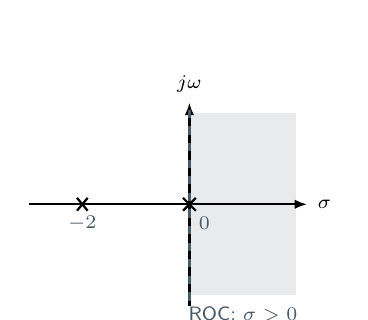
\begin{tikzpicture}[scale=0.68]
        \fill[PrimaryColor, fill opacity=0.10] (0.03,-1.7) rectangle (2.0,1.7);
        \draw[-{Latex[length=1.6mm]}, thick] (-3.0,0)--(2.2,0) node[right] {\scriptsize$\sigma$};
        \draw[-{Latex[length=1.6mm]}, thick] (0,-1.9)--(0,1.9) node[above] {\scriptsize$j\omega$};
        \draw[dashed, thick, DarkGray] (0,-1.8)--(0,1.8);
        \draw[thick] (-2.1,0.12)--(-1.9,-0.12); \draw[thick] (-2.1,-0.12)--(-1.9,0.12);
        \draw[thick] (-0.12,0.12)--(0.12,-0.12); \draw[thick] (-0.12,-0.12)--(0.12,0.12);
        \node[DarkGray] at (-2,-0.36) {\scriptsize $-2$};
        \node[DarkGray] at (0.28,-0.36) {\scriptsize $0$};
        \node[DarkGray] at (1.0,-2.05) {\scriptsize ROC: $\sigma>0$};
      \end{tikzpicture}
    \end{minipage}\hfill
    \begin{minipage}{0.55\textwidth}\centering
      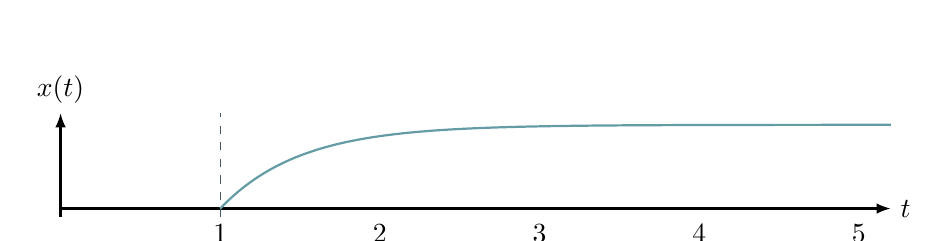
\begin{tikzpicture}
        \begin{axis}[
            width=\textwidth, height=2.9cm,
            slideaxis,
            xmin=0, xmax=5.2, ymin=-0.05, ymax=0.57,
            xtick={0,1,2,3,4,5}, ytick=\empty,
            xlabel={$t$}, ylabel={$x(t)$},
            xlabel style={anchor=west}, ylabel style={anchor=south}
          ]
          \addplot[DarkGray, dashed] coordinates {(1,-0.05) (1,0.57)};
          \addplot[AccentColor, thick, domain=1:5.2, samples=180] {0.5*(1-exp(-2*(x-1)))};
        \end{axis}
      \end{tikzpicture}
    \end{minipage}
  \end{center}
\end{examplebox}

\begin{examplebox}{Problem 8.6}
  \Prompt{Invert \(X(s)=\dfrac{2}{s(s^2+4)}\) with ROC \(\text{Re}\{s\}>0\).}

  \medskip
  \SketchLabel{}
  Define
  \[
    Y(s)=\frac{2}{s^2+4},
    \qquad
    \ROC:\ \text{Re}\{s\}>0.
  \]
  Then
  \[
    X(s)=\frac{Y(s)}{s},
    \qquad
    \ROC:\ \text{Re}\{s\}>0.
  \]
  Now use the standard sine pair directly:
  \[
    \Lpair{\sin(2t)u(t)}{\frac{2}{s^2+4}},
    \qquad
    \ROC:\ \text{Re}\{s\}>0.
  \]
  Therefore
  \[
    \Linvpair{Y(s)}{\sin(2t)u(t)},
    \qquad
    \ROC:\ \text{Re}\{s\}>0.
  \]
  Now use the integration property:
  \[
    \Linvpair{\frac{Y(s)}{s}}{\int_{-\infty}^{t} y(\tau)\,d\tau},
    \qquad
    \ROC:\ \text{Re}\{s\}>0.
  \]
  Since \(y(\tau)=\sin(2\tau)u(\tau)\) is right-sided,
  \[
    x(t)=\int_{-\infty}^{t}\sin(2\tau)u(\tau)\,d\tau
    =\int_{0}^{t}\sin(2\tau)\,d\tau \, u(t).
  \]
  Therefore
  \[
    x(t)=\left[-\frac{\cos(2\tau)}{2}\right]_{\tau=0}^{\tau=t}u(t)
    =\frac12\bigl(1-\cos(2t)\bigr)u(t),
    \qquad
    \ROC:\ \text{Re}\{s\}>0.
  \]

  \begin{center}
    \begin{minipage}{0.42\textwidth}\centering
      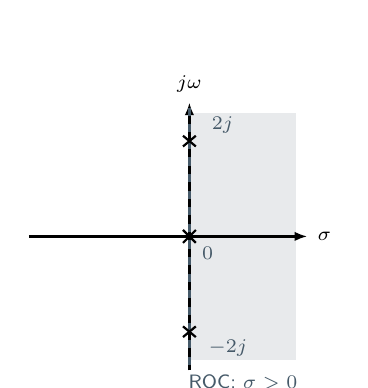
\begin{tikzpicture}[scale=0.68]
        \fill[PrimaryColor, fill opacity=0.10] (0.03,-2.3) rectangle (2.0,2.3);
        \draw[-{Latex[length=1.6mm]}, thick] (-3.0,0)--(2.2,0) node[right] {\scriptsize$\sigma$};
        \draw[-{Latex[length=1.6mm]}, thick] (0,-2.5)--(0,2.5) node[above] {\scriptsize$j\omega$};
        \draw[dashed, thick, DarkGray] (0,-2.4)--(0,2.4);
        \draw[thick] (-0.12,0.12)--(0.12,-0.12); \draw[thick] (-0.12,-0.12)--(0.12,0.12);
        \draw[thick] (-0.12,1.88)--(0.12,1.68); \draw[thick] (-0.12,1.68)--(0.12,1.88);
        \draw[thick] (-0.12,-1.68)--(0.12,-1.88); \draw[thick] (-0.12,-1.88)--(0.12,-1.68);
        \node[DarkGray] at (0.34,-0.32) {\scriptsize $0$};
        \node[DarkGray] at (0.62,2.08) {\scriptsize $2j$};
        \node[DarkGray] at (0.72,-2.08) {\scriptsize $-2j$};
        \node[DarkGray] at (1.0,-2.72) {\scriptsize ROC: $\sigma>0$};
      \end{tikzpicture}
    \end{minipage}\hfill
    \begin{minipage}{0.55\textwidth}\centering
      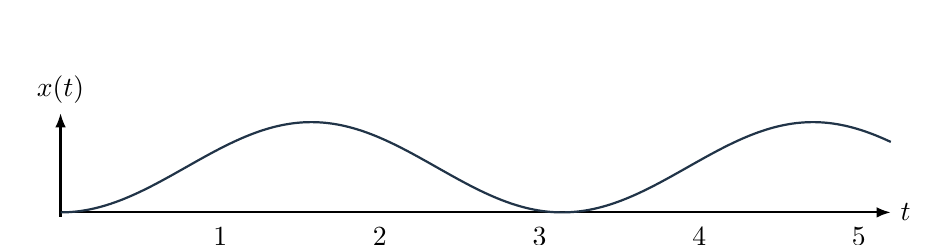
\begin{tikzpicture}
        \begin{axis}[
            width=\textwidth, height=2.9cm,
            slideaxis,
            xmin=0, xmax=5.2, ymin=-0.05, ymax=1.1,
            xtick={0,1,2,3,4,5}, ytick=\empty,
            xlabel={$t$}, ylabel={$x(t)$},
            xlabel style={anchor=west}, ylabel style={anchor=south}
          ]
          \addplot[signal, domain=0:5.2, samples=220] {0.5*(1-cos(deg(2*x)))};
        \end{axis}
      \end{tikzpicture}
    \end{minipage}
  \end{center}
\end{examplebox}

\begin{examplebox}{Problem 8.7}
  \Prompt{Invert \(X(s)=\dfrac{s}{s+2}\) with ROC \(\text{Re}\{s\}>-2\).}

  \medskip
  \SketchLabel{}
  The fraction is improper, so divide first:
  \[
    \frac{s}{s+2}=1-\frac{2}{s+2},
    \qquad
    \ROC:\ \text{Re}\{s\}>-2.
  \]
  The constant term corresponds to an impulse:
  \[
    \Linvpair{1}{\delta(t)},
    \qquad
    \ROC:\ \text{entire } s\text{-plane}.
  \]
  For the proper term,
  \[
    \Linvpair{\frac{2}{s+2}}{2e^{-2t}u(t)},
    \qquad
    \ROC:\ \text{Re}\{s\}>-2.
  \]
  Therefore
  \[
    x(t)=\delta(t)-2e^{-2t}u(t).
  \]
  The impulse term does not restrict the ROC, so the overall ROC is still
  \[
    \ROC:\ \text{Re}\{s\}>-2.
  \]
  As a check, one can also write
  \[
    \frac{s}{s+2}=s\cdot\frac{1}{s+2},
    \qquad
    \ROC:\ \text{Re}\{s\}>-2,
  \]
  and then use
  \[
    \Linvpair{\frac{1}{s+2}}{e^{-2t}u(t)},
    \qquad
    \ROC:\ \text{Re}\{s\}>-2,
  \]
  so
  \[
    \Linvpair{s\cdot\frac{1}{s+2}}{\frac{d}{dt}\bigl[e^{-2t}u(t)\bigr]}
    =\delta(t)-2e^{-2t}u(t),
    \qquad
    \ROC:\ \text{Re}\{s\}>-2.
  \]

  \begin{center}
    \begin{minipage}{0.42\textwidth}\centering
      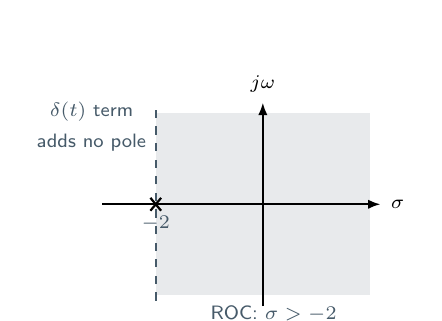
\begin{tikzpicture}[scale=0.68]
        \fill[PrimaryColor, fill opacity=0.10] (-2.0,-1.7) rectangle (2.0,1.7);
        \draw[-{Latex[length=1.6mm]}, thick] (-3.0,0)--(2.2,0) node[right] {\scriptsize$\sigma$};
        \draw[-{Latex[length=1.6mm]}, thick] (0,-1.9)--(0,1.9) node[above] {\scriptsize$j\omega$};
        \draw[dashed, thick, DarkGray] (-2,-1.8)--(-2,1.8);
        \draw[thick] (-2.1,0.12)--(-1.9,-0.12); \draw[thick] (-2.1,-0.12)--(-1.9,0.12);
        \node[DarkGray] at (-2,-0.36) {\scriptsize $-2$};
        \node[DarkGray] at (0.2,-2.05) {\scriptsize ROC: $\sigma>-2$};
        \node[DarkGray, align=center] at (-3.2,1.45) {\scriptsize $\delta(t)$ term\\[-1pt]\scriptsize adds no pole};
      \end{tikzpicture}
    \end{minipage}\hfill
    \begin{minipage}{0.55\textwidth}\centering
      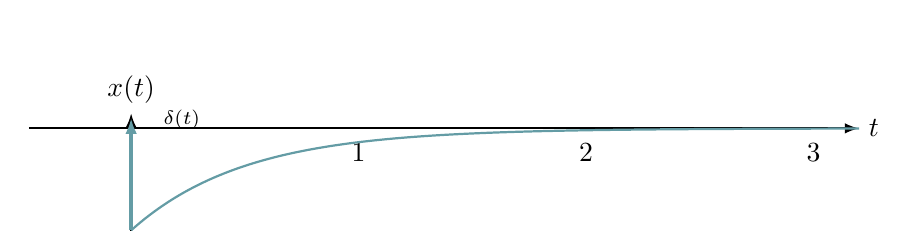
\begin{tikzpicture}
        \begin{axis}[
            width=\textwidth, height=3.2cm,
            slideaxis,
            xmin=-0.45, xmax=3.2, ymin=-2.2, ymax=0.3,
            xtick={0,1,2,3}, ytick=\empty,
            xlabel={$t$}, ylabel={$x(t)$},
            xlabel style={anchor=west}, ylabel style={anchor=south}
          ]
          \addplot[AccentColor, thick, domain=0:3.2, samples=180] {-2*exp(-2*x)};
          \draw[-{Latex[length=2mm]}, ultra thick, AccentColor] (axis cs:0,-2.0) -- (axis cs:0,0.2);
          \node[font=\scriptsize, anchor=west] at (axis cs:0.1,0.18) {$\delta(t)$};
        \end{axis}
      \end{tikzpicture}
    \end{minipage}
  \end{center}
\end{examplebox}

\newpage

\section{Applications of Laplace Transform}

\begin{examplebox}{Problem 9.1}
  \Prompt{For \(H(s)=\dfrac{s+2}{(s+1)(s+2)}\), determine the admissible ROC choices and the corresponding causality/stability properties.}

  \medskip
  \SketchLabel{}
  After cancellation,
  \[
    H(s)=\frac{1}{s+1}.
  \]
  So the only admissible ROCs are
  \[
    \text{Re}\{s\}>-1 \quad \text{or} \quad \text{Re}\{s\}<-1.
  \]
  The right-half ROC gives the causal and stable realization \(e^{-t}u(t)\). The left-half ROC gives \(-e^{-t}u(-t)\), which is anti-causal and unstable.

  \begin{center}
    \begin{minipage}{0.48\textwidth}\centering
      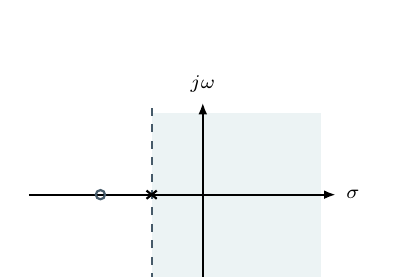
\begin{tikzpicture}[scale=0.65]
        \fill[AccentColor, fill opacity=0.12] (-1,-1.6) rectangle (2.3,1.6);
        \draw[-{Latex[length=1.5mm]}, thick] (-3.4,0)--(2.6,0) node[right] {\scriptsize$\sigma$};
        \draw[-{Latex[length=1.5mm]}, thick] (0,-1.8)--(0,1.8) node[above] {\scriptsize$j\omega$};
        \draw[dashed, thick, DarkGray] (-1,-1.7)--(-1,1.7);
        \draw[thick] (-1.1,0.08)--(-0.9,-0.08); \draw[thick] (-1.1,-0.08)--(-0.9,0.08);
        \draw[DarkGray, thick] (-2,0) circle (0.09);
      \end{tikzpicture}\\[2pt]
      {\scriptsize $\text{Re}\{s\}>-1$: causal, stable}
    \end{minipage}\hfill
    \begin{minipage}{0.48\textwidth}\centering
      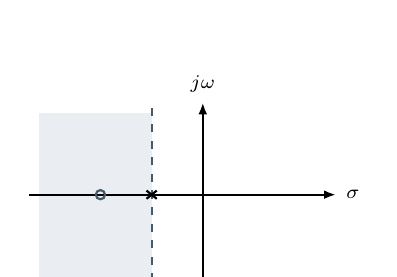
\begin{tikzpicture}[scale=0.65]
        \fill[SecondaryColor, fill opacity=0.12] (-3.2,-1.6) rectangle (-1,1.6);
        \draw[-{Latex[length=1.5mm]}, thick] (-3.4,0)--(2.6,0) node[right] {\scriptsize$\sigma$};
        \draw[-{Latex[length=1.5mm]}, thick] (0,-1.8)--(0,1.8) node[above] {\scriptsize$j\omega$};
        \draw[dashed, thick, DarkGray] (-1,-1.7)--(-1,1.7);
        \draw[thick] (-1.1,0.08)--(-0.9,-0.08); \draw[thick] (-1.1,-0.08)--(-0.9,0.08);
        \draw[DarkGray, thick] (-2,0) circle (0.09);
      \end{tikzpicture}\\[2pt]
      {\scriptsize $\text{Re}\{s\}<-1$: anti-causal, unstable}
    \end{minipage}
  \end{center}
\end{examplebox}

\begin{examplebox}{Problem 9.2}
  \Prompt{For \(H(s)=\dfrac{1}{(s+1)^2(s+3)}\), determine the admissible ROC choices and the corresponding causality/stability properties.}

  \medskip
  \SketchLabel{}
  The poles are at \(s=-1\) (double) and \(s=-3\), all in the left half-plane. Therefore
  \[
    \text{Re}\{s\}>-1 \Rightarrow \text{causal and stable (}j\omega\text{-axis included)},
  \]
  \[
    \text{Re}\{s\}<-3 \Rightarrow \text{anti-causal and unstable},
  \]
  \[
    -3<\text{Re}\{s\}<-1 \Rightarrow \text{two-sided and unstable (}j\omega\text{-axis not included)}.
  \]
  Because all poles lie in the LHP, the causal realization is also stable.

  \begin{center}
    \begin{minipage}{0.32\textwidth}\centering
      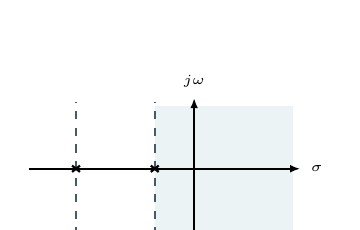
\begin{tikzpicture}[scale=0.5]
        \fill[AccentColor, fill opacity=0.12] (-1,-1.6) rectangle (2.5,1.6);
        \draw[-{Latex[length=1.3mm]}, thick] (-4.2,0)--(2.7,0) node[right] {\tiny$\sigma$};
        \draw[-{Latex[length=1.3mm]}, thick] (0,-1.8)--(0,1.8) node[above] {\tiny$j\omega$};
        \draw[dashed, thick, DarkGray] (-1,-1.7)--(-1,1.7);
        \draw[dashed, thick, DarkGray] (-3,-1.7)--(-3,1.7);
        \draw[thick] (-1.1,0.08)--(-0.9,-0.08); \draw[thick] (-1.1,-0.08)--(-0.9,0.08);
        \draw[thick] (-3.1,0.08)--(-2.9,-0.08); \draw[thick] (-3.1,-0.08)--(-2.9,0.08);
      \end{tikzpicture}\\[2pt]
      {\scriptsize $\text{Re}\{s\}>-1$: causal, stable}
    \end{minipage}\hfill
    \begin{minipage}{0.32\textwidth}\centering
      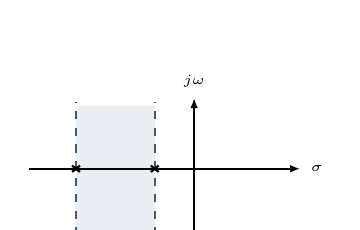
\begin{tikzpicture}[scale=0.5]
        \fill[SecondaryColor, fill opacity=0.12] (-3,-1.6) rectangle (-1,1.6);
        \draw[-{Latex[length=1.3mm]}, thick] (-4.2,0)--(2.7,0) node[right] {\tiny$\sigma$};
        \draw[-{Latex[length=1.3mm]}, thick] (0,-1.8)--(0,1.8) node[above] {\tiny$j\omega$};
        \draw[dashed, thick, DarkGray] (-1,-1.7)--(-1,1.7);
        \draw[dashed, thick, DarkGray] (-3,-1.7)--(-3,1.7);
        \draw[thick] (-1.1,0.08)--(-0.9,-0.08); \draw[thick] (-1.1,-0.08)--(-0.9,0.08);
        \draw[thick] (-3.1,0.08)--(-2.9,-0.08); \draw[thick] (-3.1,-0.08)--(-2.9,0.08);
      \end{tikzpicture}\\[2pt]
      {\scriptsize $-3<\text{Re}\{s\}<-1$: two-sided, unstable}
    \end{minipage}\hfill
    \begin{minipage}{0.32\textwidth}\centering
      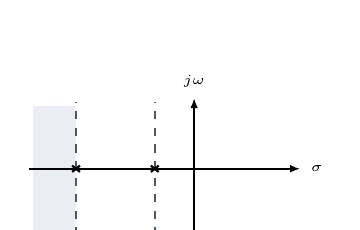
\begin{tikzpicture}[scale=0.5]
        \fill[SecondaryColor, fill opacity=0.12] (-4.1,-1.6) rectangle (-3,1.6);
        \draw[-{Latex[length=1.3mm]}, thick] (-4.2,0)--(2.7,0) node[right] {\tiny$\sigma$};
        \draw[-{Latex[length=1.3mm]}, thick] (0,-1.8)--(0,1.8) node[above] {\tiny$j\omega$};
        \draw[dashed, thick, DarkGray] (-1,-1.7)--(-1,1.7);
        \draw[dashed, thick, DarkGray] (-3,-1.7)--(-3,1.7);
        \draw[thick] (-1.1,0.08)--(-0.9,-0.08); \draw[thick] (-1.1,-0.08)--(-0.9,0.08);
        \draw[thick] (-3.1,0.08)--(-2.9,-0.08); \draw[thick] (-3.1,-0.08)--(-2.9,0.08);
      \end{tikzpicture}\\[2pt]
      {\scriptsize $\text{Re}\{s\}<-3$: anti-causal, unstable}
    \end{minipage}
  \end{center}
\end{examplebox}

\begin{examplebox}{Problem 9.3}
  \Prompt{Decide whether the Fourier transform exists for \(X(s)=\dfrac{1-e^{-3(s+2)}}{s+2}\). Interpret the result in time domain.}

  \medskip
  \SketchLabel{}
  First rewrite the transform so the delay is visible:
  \[
    X(s)=\frac{1}{s+2}-\frac{e^{-3(s+2)}}{s+2}
    =\frac{1}{s+2}-e^{-6}\frac{e^{-3s}}{s+2}.
  \]
  For the first term,
  \[
    \Linvpair{\frac{1}{s+2}}{e^{-2t}u(t)},
    \qquad
    \ROC:\ \text{Re}\{s\}>-2.
  \]
  Using the time-delay property on the same base pair,
  \[
    \Linvpair{\frac{e^{-3s}}{s+2}}{e^{-2(t-3)}u(t-3)},
    \qquad
    \ROC:\ \text{Re}\{s\}>-2.
  \]
  Therefore
  \[
    \Linvpair{e^{-6}\frac{e^{-3s}}{s+2}}{e^{-6}e^{-2(t-3)}u(t-3)}
    =e^{-2t}u(t-3).
  \]
  So the time-domain signal is
  \[
    x(t)=e^{-2t}u(t)-e^{-2t}u(t-3)
    =e^{-2t}\bigl(u(t)-u(t-3)\bigr).
  \]
  Hence
  \[
    x(t)=
    \begin{cases}
      0, & t<0,\\[2pt]
      e^{-2t}, & 0\le t<3,\\[2pt]
      0, & t\ge 3.
    \end{cases}
  \]
  So \(x(t)\) is finite-duration, supported only on \(0\le t<3\). For such a signal, the Laplace integral converges for every \(s\), so the actual ROC is the entire \(s\)-plane.

  The apparent singularity at \(s=-2\) is removable:
  \[
    \lim_{s\to-2}\frac{1-e^{-3(s+2)}}{s+2}
    =\lim_{z\to0}\frac{1-e^{-3z}}{z}
    =\lim_{z\to0} 3e^{-3z}
    =3.
  \]
  Since the actual ROC is the whole plane, it includes the \(j\omega\)-axis, so the Fourier transform exists.

  \begin{center}
    \begin{minipage}{0.40\textwidth}\centering
      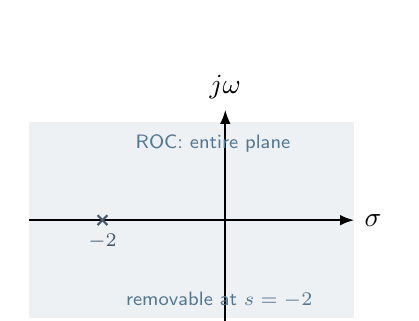
\begin{tikzpicture}[scale=0.78]
        \fill[SecondaryColor, fill opacity=0.10] (-3.2,-1.6) rectangle (2.1,1.6);
        \draw[-{Latex[length=1.8mm]}, thick] (-3.2,0)--(2.1,0) node[right] {$\sigma$};
        \draw[-{Latex[length=1.8mm]}, thick] (0,-1.8)--(0,1.8) node[above] {$j\omega$};
        \draw[DarkGray, thick] (-2.08,0.08)--(-1.92,-0.08);
        \draw[DarkGray, thick] (-2.08,-0.08)--(-1.92,0.08);
        \node[DarkGray] at (-2,-0.34) {\scriptsize $-2$};
        \node[SecondaryColor] at (-0.2,1.25) {\scriptsize ROC: entire plane};
        \node[SecondaryColor] at (-0.1,-1.3) {\scriptsize removable at \(s=-2\)};
      \end{tikzpicture}
    \end{minipage}\hfill
    \begin{minipage}{0.56\textwidth}\centering
      \begin{tikzpicture}
        \begin{axis}[
            width=\textwidth, height=3.0cm,
            slideaxis,
            xmin=-0.4, xmax=4.6, ymin=-0.02, ymax=1.08,
            xtick={0,1,2,3,4}, ytick=\empty,
            xlabel={$t$}, ylabel={$x(t)$},
            xlabel style={anchor=west}, ylabel style={anchor=south}
          ]
          \addplot[DarkGray, dashed] coordinates {(3,0) (3,0.12)};
          \addplot[signal, domain=0:3, samples=160] {exp(-2*x)};
          \addplot[signal, thick] coordinates {(3,0) (4.6,0)};
          \addplot[only marks, mark=*, mark options={fill=white, draw=PrimaryColor}, color=PrimaryColor] coordinates {(0,1) (3,0.00248)};
          \addplot[only marks, mark=*, mark options={fill=PrimaryColor, draw=PrimaryColor}, color=PrimaryColor] coordinates {(3,0)};
        \end{axis}
      \end{tikzpicture}
    \end{minipage}
  \end{center}
\end{examplebox}

\begin{examplebox}{Problem 9.4}
  \Prompt{Solve \(y'(t)+y(t)=e^{-2(t-1)}u(t-1)\) with \(y(0^-)=0\).}

  \medskip
  \SketchLabel{}
  Using \(\LT\{y'(t)\}=sY(s)\),
  \[
    sY(s)+Y(s)=\frac{e^{-s}}{s+2}
    \quad \Longrightarrow \quad
    (s+1)Y(s)=\frac{e^{-s}}{s+2}.
  \]
  Hence
  \[
    Y(s)=\frac{e^{-s}}{(s+1)(s+2)}.
  \]
  Since
  \[
    \frac{1}{(s+1)(s+2)}=\frac{1}{s+1}-\frac{1}{s+2},
  \]
  the poles are at \(-1\) and \(-2\), so the admissible ROCs are
  \[
    \text{Re}\{s\}>-1,\qquad -2<\text{Re}\{s\}<-1,\qquad \text{Re}\{s\}<-2.
  \]
  These give the three inverse candidates
  \[
    \text{Re}\{s\}>-1
    \;\Longrightarrow\;
    y_1(t)=\Bigl(e^{-(t-1)}-e^{-2(t-1)}\Bigr)u(t-1),
  \]
  \[
    -2<\text{Re}\{s\}<-1
    \;\Longrightarrow\;
    y_2(t)=-e^{-(t-1)}u(1-t)-e^{-2(t-1)}u(t-1),
  \]
  \[
    \text{Re}\{s\}<-2
    \;\Longrightarrow\;
    y_3(t)=\Bigl(e^{-2(t-1)}-e^{-(t-1)}\Bigr)u(1-t).
  \]
  Now apply the initial condition:
  \[
    y(0^-)=0.
  \]
  Only \(y_1(t)\) satisfies \(y(0^-)=0\), so the correct ROC is
  \[
    \ROC:\ \text{Re}\{s\}>-1,
  \]
  and the solution is
  \[
    y(t)=\Bigl(e^{-(t-1)}-e^{-2(t-1)}\Bigr)u(t-1).
  \]

  \begin{center}
    \begin{minipage}{0.40\textwidth}\centering
      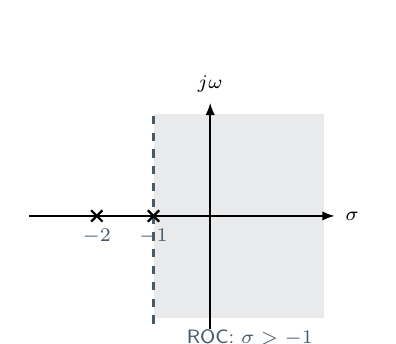
\begin{tikzpicture}[scale=0.72]
        \fill[PrimaryColor, fill opacity=0.10] (-1,-1.8) rectangle (2.0,1.8);
        \draw[-{Latex[length=1.6mm]}, thick] (-3.2,0)--(2.2,0) node[right] {\scriptsize$\sigma$};
        \draw[-{Latex[length=1.6mm]}, thick] (0,-2.0)--(0,2.0) node[above] {\scriptsize$j\omega$};
        \draw[dashed, thick, DarkGray] (-1,-1.9)--(-1,1.9);
        \draw[thick] (-1.1,0.10)--(-0.9,-0.10); \draw[thick] (-1.1,-0.10)--(-0.9,0.10);
        \draw[thick] (-2.1,0.10)--(-1.9,-0.10); \draw[thick] (-2.1,-0.10)--(-1.9,0.10);
        \node[DarkGray] at (-1,-0.36) {\scriptsize $-1$};
        \node[DarkGray] at (-2,-0.36) {\scriptsize $-2$};
        \node[DarkGray] at (0.7,-2.15) {\scriptsize ROC: $\sigma>-1$};
      \end{tikzpicture}
    \end{minipage}\hfill
    \begin{minipage}{0.56\textwidth}\centering
      \begin{tikzpicture}
        \begin{axis}[
            width=\textwidth, height=2.9cm,
            slideaxis,
            xmin=0, xmax=5.2, ymin=-0.05, ymax=0.75,
            xtick={0,1,2,3,4,5}, ytick=\empty,
            xlabel={$t$}, ylabel={$y(t)$},
            xlabel style={anchor=west}, ylabel style={anchor=south}
          ]
          \addplot[DarkGray, dashed] coordinates {(1,-0.05) (1,0.75)};
          \addplot[PrimaryColor, thick, domain=1:5.2, samples=180] {exp(-(x-1))-exp(-2*(x-1))};
        \end{axis}
      \end{tikzpicture}
    \end{minipage}
  \end{center}
\end{examplebox}

\begin{examplebox}{Problem 9.5}
  \Prompt{Solve \(y''(t)+3y'(t)+2y(t)=e^{-(t-1)}u(t-1)\) with zero initial conditions.}

  \medskip
  \SketchLabel{}
  Using \(\LT\{y'(t)\}=sY(s)\) and \(\LT\{y''(t)\}=s^2Y(s)\),
  \[
    s^2Y(s)+3sY(s)+2Y(s)=\frac{e^{-s}}{s+1}
    \quad \Longrightarrow \quad
    (s^2+3s+2)Y(s)=\frac{e^{-s}}{s+1}.
  \]
  Therefore
  \[
    Y(s)=\frac{e^{-s}}{(s+1)^2(s+2)}.
  \]
  For
  \[
    F(s)=\frac{1}{(s+1)^2(s+2)}
    =\frac{A}{s+1}+\frac{B}{(s+1)^2}+\frac{C}{s+2},
  \]
  residues give
  \[
    C=\lim_{s\to-2}(s+2)F(s)=1,
    \qquad
    B=\lim_{s\to-1}(s+1)^2F(s)=1,
  \]
  and for the simple-over-repeated coefficient,
  \[
    A=\left.\frac{d}{ds}\Big((s+1)^2F(s)\Big)\right|_{s=-1}=-1.
  \]
  Therefore
  \[
    \frac{1}{(s+1)^2(s+2)}=\frac{1}{s+2}-\frac{1}{s+1}+\frac{1}{(s+1)^2},
  \]
  so the admissible ROCs are
  \[
    \text{Re}\{s\}>-1,\qquad -2<\text{Re}\{s\}<-1,\qquad \text{Re}\{s\}<-2.
  \]
  The corresponding inverses are
  \[
    \text{Re}\{s\}>-1
    \;\Longrightarrow\;
    y_1(t)=\Bigl(e^{-2(t-1)}-e^{-(t-1)}+(t-1)e^{-(t-1)}\Bigr)u(t-1),
  \]
  \[
    -2<\text{Re}\{s\}<-1
    \;\Longrightarrow\;
    y_2(t)=e^{-2(t-1)}u(t-1)+(2-t)e^{-(t-1)}u(1-t),
  \]
  \[
    \text{Re}\{s\}<-2
    \;\Longrightarrow\;
    y_3(t)=\Bigl(-e^{-2(t-1)}+(2-t)e^{-(t-1)}\Bigr)u(1-t).
  \]
  Now use the initial conditions:
  \[
    y(0^-)=0,\qquad y'(0^-)=0,\qquad y''(0^-)=0.
  \]
  Therefore the only admissible choice is
  \[
    \ROC:\ \text{Re}\{s\}>-1.
  \]
  For this ROC the signal is zero for \(t<1\), so \(y'(0^-)=0\) also holds. Hence
  \[
    y(t)=\Bigl(e^{-2(t-1)}-e^{-(t-1)}+(t-1)e^{-(t-1)}\Bigr)u(t-1).
  \]

  \begin{center}
    \begin{minipage}{0.40\textwidth}\centering
      \begin{tikzpicture}[scale=0.72]
        \fill[PrimaryColor, fill opacity=0.10] (-1,-1.8) rectangle (2.0,1.8);
        \draw[-{Latex[length=1.6mm]}, thick] (-3.2,0)--(2.2,0) node[right] {\scriptsize$\sigma$};
        \draw[-{Latex[length=1.6mm]}, thick] (0,-2.0)--(0,2.0) node[above] {\scriptsize$j\omega$};
        \draw[dashed, thick, DarkGray] (-1,-1.9)--(-1,1.9);
        \draw[thick] (-1.1,0.10)--(-0.9,-0.10); \draw[thick] (-1.1,-0.10)--(-0.9,0.10);
        \draw[thick] (-2.1,0.10)--(-1.9,-0.10); \draw[thick] (-2.1,-0.10)--(-1.9,0.10);
        \node[DarkGray] at (-1,-0.36) {\scriptsize $-1$};
        \node[DarkGray] at (-2,-0.36) {\scriptsize $-2$};
        \node[DarkGray, align=center] at (-0.75,0.56) {\scriptsize double\\[-1pt]\scriptsize pole};
        \node[DarkGray] at (0.7,-2.15) {\scriptsize ROC: $\sigma>-1$};
      \end{tikzpicture}
    \end{minipage}\hfill
    \begin{minipage}{0.56\textwidth}\centering
      \begin{tikzpicture}
        \begin{axis}[
            width=\textwidth, height=2.9cm,
            slideaxis,
            xmin=0, xmax=5.2, ymin=-0.05, ymax=0.75,
            xtick={0,1,2,3,4,5}, ytick=\empty,
            xlabel={$t$}, ylabel={$y(t)$},
            xlabel style={anchor=west}, ylabel style={anchor=south}
          ]
          \addplot[DarkGray, dashed] coordinates {(1,-0.05) (1,0.75)};
          \addplot[AccentColor, thick, domain=1:5.2, samples=180] {exp(-2*(x-1))-exp(-(x-1))+(x-1)*exp(-(x-1))};
        \end{axis}
      \end{tikzpicture}
    \end{minipage}
  \end{center}
\end{examplebox}

\begin{examplebox}{Problem 9.6}
  \Prompt{A causal LTI system is described by the LCCDE
    \[
      \frac{d^2 y}{dt^2}+5\frac{dy}{dt}+6y(t)=\frac{dx}{dt}+3x(t).
    \]
  Find \(H(s)\), sketch the pole--zero plot, determine whether the system is stable, and find the impulse response \(h(t)\).}

  \medskip
  \SketchLabel{}
  Transform the LCCDE directly:
  \[
    s^2 Y(s)+5sY(s)+6Y(s)=sX(s)+3X(s).
  \]
  Hence
  \[
    H(s)=\frac{Y(s)}{X(s)}=\frac{s+3}{s^2+5s+6}=\frac{s+3}{(s+2)(s+3)}=\frac{1}{s+2}.
  \]
  There is a pole--zero cancellation at \(s=-3\). The remaining pole is at \(s=-2\) and there are no finite zeros.
  The algebraic form \(H(s)=1/(s+2)\) admits two possible ROCs:
  \[
    \text{Re}\{s\}>-2
    \qquad \text{or} \qquad
    \text{Re}\{s\}<-2.
  \]
  Since the system is stated to be causal, we choose
  \[
    \ROC:\ \text{Re}\{s\}>-2.
  \]
  Hence the impulse response is
  \[
    h(t)=e^{-2t}\,u(t).
  \]
  Because this ROC includes the \(j\omega\)-axis, the system is \textbf{stable}.

  \begin{center}
    \begin{tikzpicture}[scale=0.78]
      \fill[PrimaryColor, fill opacity=0.14] (-1.06,-1.9) rectangle (2.2,1.9);
      \draw[-{Latex[length=1.8mm]}, thick] (-2.2,0)--(2.2,0) node[right] {$\text{Re}\{s\}$};
      \draw[-{Latex[length=1.8mm]}, thick] (0,-2)--(0,2) node[above] {$j\omega$};
      \draw[dashed, thick, DarkGray] (-1.06,-1.9)--(-1.06,1.9);
      % cancelled pole-zero at s=-3
      \draw[thick, DarkGray] (-1.8,-0.12)--(-1.62,0.12); \draw[thick, DarkGray] (-1.8,0.12)--(-1.62,-0.12);
      \draw[thick, DarkGray] (-1.71,0) circle (0.12);
      \node[below, DarkGray] at (-1.71,-0.22) {\scriptsize $-3$};
      % pole at s=-2
      \draw[thick] (-1.14,-0.12)--(-0.98,0.12); \draw[thick] (-1.14,0.12)--(-0.98,-0.12);
      \node[below] at (-1.06,-0.16) {\scriptsize $-2$};
    \end{tikzpicture}
  \end{center}
\end{examplebox}

\section{z-Transform: Definition, Properties, ROC, Poles and Zeros}

\begin{examplebox}{Problem 10.1}
  \Prompt{Find the z-transform, poles, zeros, and ROC of \(x[n]=\left(\frac34\right)^n\cos\!\left(\frac{\pi n}{3}\right)u[n]\).}

  \medskip
  \SketchLabel{}
  Using Euler's formula,
  \[
    x[n]=\frac12\!\left(\frac34 e^{j\pi/3}\right)^{\!n} u[n]+\frac12\!\left(\frac34 e^{-j\pi/3}\right)^{\!n} u[n].
  \]
  Transform the first part:
  \[
    \Zpair{\frac12\!\left(\frac34 e^{j\pi/3}\right)^{\!n} u[n]}
    {\frac{\frac12}{1-\frac34 e^{j\pi/3}z^{-1}}},
    \qquad
    \ROC:\ |z|>\frac34.
  \]
  Transform the second part:
  \[
    \Zpair{\frac12\!\left(\frac34 e^{-j\pi/3}\right)^{\!n} u[n]}
    {\frac{\frac12}{1-\frac34 e^{-j\pi/3}z^{-1}}},
    \qquad
    \ROC:\ |z|>\frac34.
  \]
  Therefore
  \[
    X(z)=\frac{\frac12}{1-\frac34 e^{j\pi/3}z^{-1}}
    +\frac{\frac12}{1-\frac34 e^{-j\pi/3}z^{-1}},
    \qquad
    \ROC:\ |z|>\frac34.
  \]
  Combine over a common denominator:
  \[
    X(z)=\frac{\frac12\!\left(1-\frac34 e^{-j\pi/3}z^{-1}\right)
    +\frac12\!\left(1-\frac34 e^{j\pi/3}z^{-1}\right)}
    {\left(1-\frac34 e^{j\pi/3}z^{-1}\right)\left(1-\frac34 e^{-j\pi/3}z^{-1}\right)}.
  \]
  Since
  \[
    e^{j\pi/3}+e^{-j\pi/3}=2\cos\!\left(\frac{\pi}{3}\right)=1,
    \qquad
    e^{j\pi/3}e^{-j\pi/3}=1,
  \]
  we obtain
  \[
    X(z)=\frac{1-\frac38 z^{-1}}{1-\frac34 z^{-1}+\frac{9}{16}z^{-2}},
    \qquad
    \ROC:\ |z|>\frac34.
  \]
  Poles: \(z=\frac34 e^{\pm j\pi/3}\). Zeros: \(z=0,\frac38\).

  \begin{center}
    \begin{tikzpicture}[scale=0.78]
      \fill[PrimaryColor, fill opacity=0.14, even odd rule] (-1.9,-1.9) rectangle (1.9,1.9) (0,0) circle (0.97);
      \draw[-{Latex[length=1.8mm]}, thick] (-2,0)--(2,0) node[right] {$\text{Re}\{z\}$};
      \draw[-{Latex[length=1.8mm]}, thick] (0,-2)--(0,2) node[above] {$\text{Im}\{z\}$};
      \draw[PrimaryColor, thick] (0,0) circle (1.3);
      \draw[dashed, thick, DarkGray] (0,0) circle (0.97);
      \draw[thick] (0.41,0.92)--(0.57,0.76); \draw[thick] (0.41,0.76)--(0.57,0.92);
      \draw[thick] (0.41,-0.76)--(0.57,-0.92); \draw[thick] (0.41,-0.92)--(0.57,-0.76);
      \draw[thick] (0,0) circle (0.07); \draw[thick] (0.49,0) circle (0.07);
    \end{tikzpicture}
  \end{center}
\end{examplebox}

\begin{examplebox}{Problem 10.2}
  \Prompt{Find the z-transform and ROC of \(x[n]=(n-2)\left(\frac13\right)^{n-2}u[n-2]\).}

  \medskip
  \SketchLabel{}
  Start from the geometric sequence
  \[
    g[n]=\left(\frac13\right)^n u[n].
  \]
  Then
  \[
    \Zpair{g[n]}{\frac{1}{1-\frac13 z^{-1}}},
    \qquad
    \ROC:\ |z|>\frac13.
  \]
  Using the differentiation property,
  \[
    \Zpair{n\,g[n]}{-z\frac{d}{dz}G(z)},
    \qquad
    \ROC:\ |z|>\frac13.
  \]
  Since
  \[
    G(z)=\frac{1}{1-\frac13 z^{-1}},
    \qquad
    -z\frac{dG}{dz}
    =-z\frac{d}{dz}\left(1-\frac13 z^{-1}\right)^{-1}
    =\frac{\frac13 z^{-1}}{\left(1-\frac13 z^{-1}\right)^2},
  \]
  we obtain
  \[
    \Zpair{n\left(\frac13\right)^n u[n]}{\frac{\frac13 z^{-1}}{\left(1-\frac13 z^{-1}\right)^2}},
    \qquad
    \ROC:\ |z|>\frac13.
  \]
  Therefore, with
  \[
    x_0[n]=n\left(\frac13\right)^n u[n],
  \]
  we have
  \[
    X_0(z)=\frac{\frac13 z^{-1}}{\left(1-\frac13 z^{-1}\right)^2},
    \qquad
    \ROC:\ |z|>\frac13.
  \]
  Since \(x[n]=x_0[n-2]\),
  \[
    X(z)=z^{-2}\frac{\frac13 z^{-1}}{\left(1-\frac13 z^{-1}\right)^2},
    \qquad
    \ROC:\ |z|>\frac13.
  \]
  In positive-power form,
  \[
    X(z)=\frac{1}{3z\left(z-\frac13\right)^2},
  \]
  so the two-sample delay contributes a pole at \(z=0\), and the repeated factor gives a double pole at \(z=\frac13\).

  \begin{center}
    \begin{tikzpicture}[scale=0.78]
      \fill[SecondaryColor, fill opacity=0.14, even odd rule] (-1.9,-1.9) rectangle (1.9,1.9) (0,0) circle (0.5);
      \draw[-{Latex[length=1.8mm]}, thick] (-1.95,0)--(1.95,0) node[right] {$\text{Re}\{z\}$};
      \draw[-{Latex[length=1.8mm]}, thick] (0,-1.95)--(0,1.95) node[above] {$\text{Im}\{z\}$};
      \draw[PrimaryColor, thick] (0,0) circle (1.3);
      \draw[dashed, thick, DarkGray] (0,0) circle (0.5);
      \draw[thick] (-0.08,0.08)--(0.08,-0.08); \draw[thick] (-0.08,-0.08)--(0.08,0.08);
      \draw[thick] (0.42,0.08)--(0.58,-0.08); \draw[thick] (0.42,-0.08)--(0.58,0.08);
      \node[DarkGray] at (0.96,0.28) {\scriptsize double pole};
    \end{tikzpicture}
  \end{center}
\end{examplebox}

\begin{examplebox}{Problem 10.3}
  \Prompt{Find the z-transform, poles, zeros, and ROC of \(x[n]=\left(\frac14\right)^n u[n]-2^n u[-n-1]\).}

  \medskip
  \SketchLabel{}
  Split the sequence into
  \[
    x_1[n]=\left(\frac14\right)^n u[n],
    \qquad
    x_2[n]=-2^n u[-n-1].
  \]
  For the right-sided part,
  \[
    \Zpair{x_1[n]}{\frac{1}{1-\frac14 z^{-1}}},
    \qquad
    \ROC:\ |z|>\frac14.
  \]
  For the left-sided part,
  \[
    \Zpair{x_2[n]}{\frac{1}{1-2 z^{-1}}},
    \qquad
    \ROC:\ |z|<2.
  \]
  Therefore
  \[
    X(z)=\frac{1}{1-\frac14 z^{-1}}+\frac{1}{1-2 z^{-1}},
    \qquad
    \ROC:\ \frac14<|z|<2.
  \]
  Combine the two terms:
  \[
    X(z)=\frac{\left(1-2z^{-1}\right)+\left(1-\frac14 z^{-1}\right)}
    {\left(1-\frac14 z^{-1}\right)\left(1-2z^{-1}\right)}
    =\frac{2\left(1-\frac98 z^{-1}\right)}
    {\left(1-\frac14 z^{-1}\right)\left(1-2z^{-1}\right)}.
  \]
  Poles: \(z=\frac14,2\). Zeros: \(z=0,\frac98\).

  \begin{center}
    \begin{tikzpicture}[scale=0.78]
      \fill[AccentColor, fill opacity=0.14, even odd rule] (0,0) circle (1.55) (0,0) circle (0.4);
      \draw[-{Latex[length=1.8mm]}, thick] (-2.05,0)--(2.05,0) node[right] {$\text{Re}\{z\}$};
      \draw[-{Latex[length=1.8mm]}, thick] (0,-2.05)--(0,2.05) node[above] {$\text{Im}\{z\}$};
      \draw[PrimaryColor, thick] (0,0) circle (1.25);
      \draw[dashed, thick, DarkGray] (0,0) circle (0.4);
      \draw[dashed, thick, DarkGray] (0,0) circle (1.55);
      \draw[thick] (0.32,0.08)--(0.48,-0.08); \draw[thick] (0.32,-0.08)--(0.48,0.08);
      \draw[thick] (1.47,0.08)--(1.63,-0.08); \draw[thick] (1.47,-0.08)--(1.63,0.08);
      \draw[thick] (0,0) circle (0.07);
      \draw[thick] (1.35,0) circle (0.07);
    \end{tikzpicture}
  \end{center}
\end{examplebox}

\begin{examplebox}{Problem 10.4}
  \Prompt{Find the z-transform and zero pattern of \(x[n]=\delta[n]-2\delta[n-1]+2\delta[n-2]-\delta[n-3]\).}

  \medskip
  \SketchLabel{}
  \[
    X(z)=1-2z^{-1}+2z^{-2}-z^{-3}.
  \]
  Multiplying by \(z^3\),
  \[
    z^3X(z)=z^3-2z^2+2z-1=(z-1)(z^2-z+1).
  \]
  Hence
  \[
    X(z)=\frac{(z-1)(z^2-z+1)}{z^3}.
  \]
  So the zeros are
  \[
    z=1,\qquad z=e^{j\pi/3},\qquad z=e^{-j\pi/3},
  \]
  and the factor \(z^3\) in the denominator gives a pole of order \(3\) at \(z=0\). Since the sequence is finite and right-sided,
  \[
    \ROC:\ \mathbb{C}\setminus\{0\}.
  \]

  \begin{center}
    \begin{tikzpicture}[scale=0.82]
      \draw[-{Latex[length=1.8mm]}, thick] (-2.1,0)--(2.1,0) node[right] {$\text{Re}\{z\}$};
      \draw[-{Latex[length=1.8mm]}, thick] (0,-2.1)--(0,2.1) node[above] {$\text{Im}\{z\}$};
      \draw[PrimaryColor, thick] (0,0) circle (1.55);
      \draw[thick] (-0.08,0.08)--(0.08,-0.08); \draw[thick] (-0.08,-0.08)--(0.08,0.08);
      \draw[thick] (1.55,0) circle (0.07);
      \draw[thick] (0.78,1.35) circle (0.07);
      \draw[thick] (0.78,-1.35) circle (0.07);
      \node[DarkGray] at (-0.18,-0.22) {\scriptsize pole at \(0\)};
    \end{tikzpicture}
  \end{center}
\end{examplebox}

\begin{examplebox}{Problem 10.5}
  \Prompt{Find the z-transform, poles, zeros, and ROC of \(x[n]=\left(\frac12\right)^{n-1}\cos\!\left(\frac{\pi(n-1)}{3}\right)u[n-1]\).}

  \medskip
  \SketchLabel{}
  First define the undelayed sequence
  \[
    x_0[n]=\left(\frac12\right)^n\cos\!\left(\frac{\pi n}{3}\right)u[n].
  \]
  Using Euler's formula,
  \[
    x_0[n]=\frac12\!\left(\frac12 e^{j\pi/3}\right)^{\!n}u[n]
    +\frac12\!\left(\frac12 e^{-j\pi/3}\right)^{\!n}u[n].
  \]
  Transform the first part:
  \[
    \Zpair{\frac12\!\left(\frac12 e^{j\pi/3}\right)^{\!n}u[n]}
    {\frac{\frac12}{1-\frac12 e^{j\pi/3}z^{-1}}},
    \qquad
    \ROC:\ |z|>\frac12.
  \]
  Transform the second part:
  \[
    \Zpair{\frac12\!\left(\frac12 e^{-j\pi/3}\right)^{\!n}u[n]}
    {\frac{\frac12}{1-\frac12 e^{-j\pi/3}z^{-1}}},
    \qquad
    \ROC:\ |z|>\frac12.
  \]
  Therefore
  \[
    X_0(z)=\frac{\frac12}{1-\frac12 e^{j\pi/3}z^{-1}}
    +\frac{\frac12}{1-\frac12 e^{-j\pi/3}z^{-1}},
    \qquad
    \ROC:\ |z|>\frac12.
  \]
  Combining the terms gives
  \[
    X_0(z)=\frac{1-\frac14 z^{-1}}{1-\frac12 z^{-1}+\frac14 z^{-2}},
    \qquad
    \ROC:\ |z|>\frac12.
  \]
  A unit delay gives
  \[
    X(z)=z^{-1}X_0(z)
    =\frac{z^{-1}\left(1-\frac14 z^{-1}\right)}{1-\frac12 z^{-1}+\frac14 z^{-2}},
    \qquad
    \ROC:\ |z|>\frac12.
  \]
  In positive-power form,
  \[
    X(z)=\frac{z-\frac14}{z^2-\frac12 z+\frac14},
  \]
  so the poles are \(z=\frac12e^{\pm j\pi/3}\) and the only finite zero is \(z=\frac14\).
  The undelayed \(X_0(z)\) had a zero at \(z=0\), but the extra factor \(z^{-1}\) from the delay removes that origin zero.

  \begin{center}
    \begin{tikzpicture}[scale=0.78]
      \fill[PrimaryColor, fill opacity=0.14, even odd rule] (-1.9,-1.9) rectangle (1.9,1.9) (0,0) circle (0.75);
      \draw[-{Latex[length=1.8mm]}, thick] (-2,0)--(2,0) node[right] {$\text{Re}\{z\}$};
      \draw[-{Latex[length=1.8mm]}, thick] (0,-2)--(0,2) node[above] {$\text{Im}\{z\}$};
      \draw[PrimaryColor, thick] (0,0) circle (1.3);
      \draw[dashed, thick, DarkGray] (0,0) circle (0.75);
      \draw[thick] (0.25,0.65)--(0.4,0.5); \draw[thick] (0.25,0.5)--(0.4,0.65);
      \draw[thick] (0.25,-0.65)--(0.4,-0.5); \draw[thick] (0.25,-0.5)--(0.4,-0.65);
      \draw[thick] (0.38,0) circle (0.07);
    \end{tikzpicture}
  \end{center}
\end{examplebox}

\newpage

\begin{examplebox}{Problem 10.6}
  \Prompt{Find the z-transform, poles, zeros, and ROC of \(y[n]=\bigl(\left(\frac12\right)^n u[n]\bigr)*\bigl(\left(\frac13\right)^n u[n]\bigr)\).}

  \medskip
  \SketchLabel{}
  By the \textbf{convolution property}, convolution in time becomes multiplication in the \(z\)-domain:
  \[
    \Zpair{\left(\tfrac12\right)^n u[n]}{\frac{1}{1-\frac12 z^{-1}}},\quad \ROC:\ |z|>\tfrac12,
  \]
  \[
    \Zpair{\left(\tfrac13\right)^n u[n]}{\frac{1}{1-\frac13 z^{-1}}},\quad \ROC:\ |z|>\tfrac13.
  \]
  Therefore
  \[
    Y(z)=\frac{1}{(1-\frac12 z^{-1})(1-\frac13 z^{-1})},
    \qquad
    \ROC:\ |z|>\tfrac12\;\;\text{(intersection)}.
  \]
  In positive-power form,
  \[
    Y(z)=\frac{z^2}{\left(z-\frac12\right)\left(z-\frac13\right)},
  \]
  so the poles are \(z=\frac12,\frac13\) and there is a double zero at \(z=0\).

  % \textbf{Verification via partial fractions:}
  % \[
  %   Y(z)=\frac{A}{1-\frac12 z^{-1}}+\frac{B}{1-\frac13 z^{-1}}.
  % \]
  % Let \(r=z^{-1}\). Then
  % \[
  %   A=\left.(1-\tfrac12 r)\frac{1}{(1-\frac12 r)(1-\frac13 r)}\right|_{r=2}=3,
  %   \qquad
  %   B=\left.(1-\tfrac13 r)\frac{1}{(1-\frac12 r)(1-\frac13 r)}\right|_{r=3}=-2.
  % \]
  % So
  % \[
  %   Y(z)=\frac{3}{1-\frac12 z^{-1}}-\frac{2}{1-\frac13 z^{-1}}
  %   \quad\Longrightarrow\quad
  %   y[n]=3\!\left(\tfrac12\right)^n u[n]-2\!\left(\tfrac13\right)^n u[n].
  % \]

  \begin{center}
    \begin{tikzpicture}[scale=0.78]
      \fill[PrimaryColor, fill opacity=0.14, even odd rule] (-1.9,-1.9) rectangle (1.9,1.9) (0,0) circle (0.65);
      \draw[-{Latex[length=1.8mm]}, thick] (-2,0)--(2,0) node[right] {$\text{Re}\{z\}$};
      \draw[-{Latex[length=1.8mm]}, thick] (0,-2)--(0,2) node[above] {$\text{Im}\{z\}$};
      \draw[PrimaryColor, thick] (0,0) circle (1.3);
      \draw[dashed, thick, DarkGray] (0,0) circle (0.65);
      \draw[thick] (0,0) circle (0.07);
      \draw[thick] (0.57,0.08)--(0.73,-0.08); \draw[thick] (0.57,-0.08)--(0.73,0.08);
      \draw[thick] (0.35,0.08)--(0.51,-0.08); \draw[thick] (0.35,-0.08)--(0.51,0.08);
      \node[DarkGray] at (-0.68,0.26) {\scriptsize double zero};
      \node[DarkGray] at (0.65,-0.3) {\scriptsize $\frac12$};
      \node[DarkGray] at (0.43,-0.3) {\scriptsize $\frac13$};
    \end{tikzpicture}
  \end{center}
\end{examplebox}

\begin{examplebox}{Problem 10.7}
  \Prompt{Let \(x[n]=\left(\frac12\right)^n u[n]\). Find the z-transform and ROC of the running sum \(y[n]=\displaystyle\sum_{k=-\infty}^{n}x[k]\).}

  \medskip
  \SketchLabel{}
  First transform the input:
  \[
    \Zpair{\left(\frac12\right)^n u[n]}{\frac{1}{1-\frac12 z^{-1}}},
    \qquad
    \ROC:\ |z|>\frac12.
  \]
  So
  \[
    X(z)=\frac{1}{1-\frac12 z^{-1}},
    \qquad
    \ROC:\ |z|>\frac12.
  \]
  By the \textbf{accumulation property},
  \[
    \Zpair{u[n]}{\frac{1}{1-z^{-1}}},
    \qquad
    \ROC:\ |z|>1.
  \]
  Therefore
  \[
    Y(z)=\frac{X(z)}{1-z^{-1}}=\frac{1}{(1-z^{-1})(1-\frac12 z^{-1})},
    \qquad
    \ROC:\ |z|>1.
  \]
  The new pole at \(z=1\) from the accumulator restricts the ROC to \(|z|>1\).
  In positive-power form,
  \[
    Y(z)=\frac{z^2}{(z-1)\left(z-\frac12\right)},
  \]
  so there is also a double zero at \(z=0\).

  % \textbf{Verification:}
  % \[
  %   Y(z)=\frac{A}{1-z^{-1}}+\frac{B}{1-\frac12 z^{-1}}.
  % \]
  % With \(r=z^{-1}\),
  % \[
  %   A=\left.(1-r)\frac{1}{(1-r)(1-\frac12 r)}\right|_{r=1}=2,
  %   \qquad
  %   B=\left.(1-\tfrac12 r)\frac{1}{(1-r)(1-\frac12 r)}\right|_{r=2}=-1.
  % \]
  % Hence
  % \[
  %   Y(z)=\frac{2}{1-z^{-1}}-\frac{1}{1-\frac12 z^{-1}},
  % \]
  % so \(y[n]=\bigl(2-\left(\frac12\right)^n\bigr)u[n]\).
  % Check: \(y[0]=1\), \(y[1]=\frac32\), \(y[\infty]\to2\).

  \begin{center}
    \begin{tikzpicture}[scale=0.78]
      \fill[SecondaryColor, fill opacity=0.14, even odd rule] (-1.9,-1.9) rectangle (1.9,1.9) (0,0) circle (1.3);
      \draw[-{Latex[length=1.8mm]}, thick] (-2,0)--(2,0) node[right] {$\text{Re}\{z\}$};
      \draw[-{Latex[length=1.8mm]}, thick] (0,-2)--(0,2) node[above] {$\text{Im}\{z\}$};
      \draw[PrimaryColor, thick] (0,0) circle (1.3);
      \draw[dashed, thick, DarkGray] (0,0) circle (1.3);
      \draw[thick] (0,0) circle (0.07);
      \draw[thick] (1.22,0.08)--(1.38,-0.08); \draw[thick] (1.22,-0.08)--(1.38,0.08);
      \draw[thick] (0.57,0.08)--(0.73,-0.08); \draw[thick] (0.57,-0.08)--(0.73,0.08);
      \node[DarkGray] at (-0.68,0.26) {\scriptsize double zero};
      \node[DarkGray] at (1.3,-0.35) {\scriptsize $1$};
      \node[DarkGray] at (0.65,-0.35) {\scriptsize $\frac12$};
    \end{tikzpicture}
  \end{center}
\end{examplebox}

\newpage

\section{Inverse z-Transform}

\begin{examplebox}{Problem 11.1}
  \Prompt{Invert \(X(z)=\dfrac{2-z^{-1}}{(1-\frac14 z^{-1})(1-\frac34 z^{-1})}\) for \(|z|>\frac34\).}

  \medskip
  \SketchLabel{}
  Partial fractions:
  \[
    X(z)=\frac{A}{1-\frac14 z^{-1}}+\frac{B}{1-\frac34 z^{-1}}.
  \]
  Let \(r=z^{-1}\). Then
  \[
    A=\left.(1-\tfrac14 r)\frac{2-r}{(1-\frac14 r)(1-\frac34 r)}\right|_{r=4}=1,
    \qquad
    B=\left.(1-\tfrac34 r)\frac{2-r}{(1-\frac14 r)(1-\frac34 r)}\right|_{r=\frac43}=1.
  \]
  Therefore
  \[
    \frac{2-z^{-1}}{(1-\frac14 z^{-1})(1-\frac34 z^{-1})}
    =\frac{1}{1-\frac14 z^{-1}}+\frac{1}{1-\frac34 z^{-1}}.
  \]
  Since \(|z|>3/4\), both terms are right-sided:
  \[
    x[n]=\left(\frac14\right)^n u[n]+\left(\frac34\right)^n u[n].
  \]
  In positive-power form,
  \[
    X(z)=\frac{z(2z-1)}{\left(z-\frac14\right)\left(z-\frac34\right)},
  \]
  so the zeros are at \(z=0\) and \(z=\frac12\).

  \begin{center}
    \begin{minipage}{0.42\textwidth}\centering
      \begin{tikzpicture}[scale=0.78]
        \fill[AccentColor, fill opacity=0.12, even odd rule] (-1.9,-1.9) rectangle (1.9,1.9) (0,0) circle (0.98);
        \draw[-{Latex[length=1.8mm]}, thick] (-2.0,0)--(2.0,0) node[right] {$\text{Re}\{z\}$};
        \draw[-{Latex[length=1.8mm]}, thick] (0,-2.0)--(0,2.0) node[above] {$\text{Im}\{z\}$};
        \draw[PrimaryColor, thick] (0,0) circle (1.3);
        \draw[dashed, thick, DarkGray] (0,0) circle (0.33);
        \draw[dashed, thick, DarkGray] (0,0) circle (0.98);
        \draw[thick] (0,0) circle (0.07);
        \draw[thick] (0.58,0) circle (0.07);
        \draw[thick] (0.25,0.08)--(0.41,-0.08); \draw[thick] (0.25,-0.08)--(0.41,0.08);
        \draw[thick] (0.90,0.08)--(1.06,-0.08); \draw[thick] (0.90,-0.08)--(1.06,0.08);
        \node[DarkGray] at (0.33,-0.25) {\scriptsize $\frac14$};
        \node[DarkGray] at (0.65,0.24) {\scriptsize $\frac12$};
        \node[DarkGray] at (0.98,-0.25) {\scriptsize $\frac34$};
      \end{tikzpicture}
    \end{minipage}\hfill
    \begin{minipage}{0.55\textwidth}\centering
      \ZTSequencePlot{-1.2}{8.2}{-0.05}{2.15}{-1,0,...,8}{x >= 0 ? pow(0.25,x) + pow(0.75,x) : 0}
    \end{minipage}
  \end{center}
\end{examplebox}

\begin{examplebox}{Problem 11.2}
  \Prompt{Invert \(X(z)=\dfrac{1}{(1-2z^{-1})(1-\frac13 z^{-1})}\) for \(\frac13<|z|<2\).}

  \medskip
  \SketchLabel{}
  Partial fractions:
  \[
    X(z)=\frac{A}{1-2z^{-1}}+\frac{B}{1-\frac13 z^{-1}}.
  \]
  Let \(r=z^{-1}\). Then
  \[
    A=\left.(1-2r)\frac{1}{(1-2r)(1-\frac13 r)}\right|_{r=\frac12}=\frac65,
    \qquad
    B=\left.(1-\tfrac13 r)\frac{1}{(1-2r)(1-\frac13 r)}\right|_{r=3}=-\frac15.
  \]
  So
  \[
    \frac{1}{(1-2z^{-1})(1-\frac13 z^{-1})}
    =\frac{6/5}{1-2z^{-1}}-\frac{1/5}{1-\frac13 z^{-1}}.
  \]
  With \(\frac13<|z|<2\), the pole at \(z=2\) gives a left-sided term and the pole at \(z=\frac13\) gives a right-sided term:
  \[
    x[n]=-\frac{6}{5}\cdot 2^n\,u[-n-1]-\frac{1}{5}\left(\frac13\right)^n u[n].
  \]
  In positive-power form,
  \[
    X(z)=\frac{z^2}{(z-2)\left(z-\frac13\right)},
  \]
  so there is a double zero at \(z=0\).

  \begin{center}
    \begin{minipage}{0.42\textwidth}\centering
      \begin{tikzpicture}[scale=0.78]
        \fill[AccentColor, fill opacity=0.14, even odd rule] (0,0) circle (1.55) (0,0) circle (0.5);
        \draw[-{Latex[length=1.8mm]}, thick] (-2.05,0)--(2.05,0) node[right] {$\text{Re}\{z\}$};
        \draw[-{Latex[length=1.8mm]}, thick] (0,-2.05)--(0,2.05) node[above] {$\text{Im}\{z\}$};
        \draw[PrimaryColor, thick] (0,0) circle (1.3);
        \draw[dashed, thick, DarkGray] (0,0) circle (0.5);
        \draw[dashed, thick, DarkGray] (0,0) circle (1.55);
        \draw[thick] (0,0) circle (0.07);
        \draw[thick] (0.42,0.08)--(0.58,-0.08); \draw[thick] (0.42,-0.08)--(0.58,0.08);
        \draw[thick] (1.47,0.08)--(1.63,-0.08); \draw[thick] (1.47,-0.08)--(1.63,0.08);
        \node[DarkGray] at (-0.72,0.28) {\scriptsize double zero};
      \end{tikzpicture}
    \end{minipage}\hfill
    \begin{minipage}{0.55\textwidth}\centering
      \ZTSequencePlot{-5.2}{5.2}{-0.24}{0.03}{-5,-4,...,5}{(x <= -1 ? -(6/5)*pow(2,x) : 0) + (x >= 0 ? -(1/5)*pow(0.3333333333,x) : 0)}
    \end{minipage}
  \end{center}
\end{examplebox}

\newpage

\begin{examplebox}{Problem 11.3}
  \Prompt{Invert \(X(z)=\dfrac{1-\frac56 z^{-1}}{(1-\frac12 z^{-1})(1-\frac13 z^{-1})}\) for \(|z|<\frac13\).}

  \medskip
  \SketchLabel{}
  Partial fractions:
  \[
    X(z)=\frac{A}{1-\frac12 z^{-1}}+\frac{B}{1-\frac13 z^{-1}}.
  \]
  Let \(r=z^{-1}\). Then
  \[
    A=\left.(1-\tfrac12 r)\frac{1-\frac56 r}{(1-\frac12 r)(1-\frac13 r)}\right|_{r=2}=-2,
    \qquad
    B=\left.(1-\tfrac13 r)\frac{1-\frac56 r}{(1-\frac12 r)(1-\frac13 r)}\right|_{r=3}=3.
  \]
  Therefore
  \[
    \frac{1-\frac56 z^{-1}}{(1-\frac12 z^{-1})(1-\frac13 z^{-1})}
    =\frac{-2}{1-\frac12 z^{-1}}+\frac{3}{1-\frac13 z^{-1}}.
  \]
  With \(|z|<\frac13\), both poles are outside the ROC, so both terms are left-sided:
  \[
    x[n]=2\left(\frac12\right)^n u[-n-1]-3\left(\frac13\right)^n u[-n-1].
  \]
  In positive-power form,
  \[
    X(z)=\frac{z\left(z-\frac56\right)}{\left(z-\frac12\right)\left(z-\frac13\right)},
  \]
  so the zeros are at \(z=0\) and \(z=\frac56\).

  \begin{center}
    \begin{minipage}{0.42\textwidth}\centering
      \begin{tikzpicture}[scale=0.78]
        \fill[SecondaryColor, fill opacity=0.14] (0,0) circle (0.5);
        \draw[-{Latex[length=1.8mm]}, thick] (-2.05,0)--(2.05,0) node[right] {$\text{Re}\{z\}$};
        \draw[-{Latex[length=1.8mm]}, thick] (0,-2.05)--(0,2.05) node[above] {$\text{Im}\{z\}$};
        \draw[PrimaryColor, thick] (0,0) circle (1.3);
        \draw[dashed, thick, DarkGray] (0,0) circle (0.5);
        \draw[dashed, thick, DarkGray] (0,0) circle (0.75);
        \draw[thick] (0,0) circle (0.07);
        \draw[thick] (1.01,0) circle (0.07);
        \draw[thick] (0.42,0.08)--(0.58,-0.08); \draw[thick] (0.42,-0.08)--(0.58,0.08);
        \draw[thick] (0.67,0.08)--(0.83,-0.08); \draw[thick] (0.67,-0.08)--(0.83,0.08);
        \node[DarkGray] at (1.08,0.24) {\scriptsize $\frac56$};
      \end{tikzpicture}
    \end{minipage}\hfill
    \begin{minipage}{0.55\textwidth}\centering
      \ZTSequencePlot{-3.2}{4.2}{-72}{6}{-3,-2,...,4}{x <= -1 ? 2*pow(0.5,x) - 3*pow(0.3333333333,x) : 0}
    \end{minipage}
  \end{center}
\end{examplebox}

\begin{examplebox}{Problem 11.4}
  \Prompt{Invert \(X(z)=\dfrac{1+\frac12 z^{-1}}{\left(1-\frac12 z^{-1}\right)^2}\) for \(|z|>\frac12\).}

  \medskip
  \SketchLabel{}
  Write
  \[
    \frac{1+\frac12 z^{-1}}{\left(1-\frac12 z^{-1}\right)^2}
    =\frac{1}{1-\frac12 z^{-1}}+\frac{z^{-1}}{\left(1-\frac12 z^{-1}\right)^2}.
  \]
  Now invert each part separately.
  For the first term,
  \[
    \Zinvpair{\frac{1}{1-\frac12 z^{-1}}}{\left(\frac12\right)^n u[n]},
    \qquad
    \ROC:\ |z|>\frac12.
  \]
  For the second term, start from the repeated-pole pair
  \[
    \Zpair{n\left(\frac12\right)^n u[n]}{\frac{\frac12 z^{-1}}{\left(1-\frac12 z^{-1}\right)^2}},
    \qquad
    \ROC:\ |z|>\frac12.
  \]
  Multiplying by \(2\),
  \[
    \Zinvpair{\frac{z^{-1}}{\left(1-\frac12 z^{-1}\right)^2}}{2n\left(\frac12\right)^n u[n]},
    \qquad
    \ROC:\ |z|>\frac12.
  \]
  Therefore
  \[
    x[n]=\left(\frac12\right)^n u[n]+2n\left(\frac12\right)^n u[n]
    =(2n+1)\left(\frac12\right)^n u[n].
  \]
  Since the sequence is right-sided, the ROC stays outside the repeated pole:
  \[
    \ROC:\ |z|>\frac12.
  \]
  In positive-power form,
  \[
    X(z)=\frac{z\left(z+\frac12\right)}{\left(z-\frac12\right)^2},
  \]
  so the zeros are at \(z=0\) and \(z=-\frac12\).

  \begin{center}
    \begin{minipage}{0.42\textwidth}\centering
      \begin{tikzpicture}[scale=0.78]
        \fill[AccentColor, fill opacity=0.12, even odd rule] (-1.9,-1.9) rectangle (1.9,1.9) (0,0) circle (0.65);
        \draw[-{Latex[length=1.8mm]}, thick] (-2.0,0)--(2.0,0) node[right] {$\text{Re}\{z\}$};
        \draw[-{Latex[length=1.8mm]}, thick] (0,-2.0)--(0,2.0) node[above] {$\text{Im}\{z\}$};
        \draw[PrimaryColor, thick] (0,0) circle (1.3);
        \draw[dashed, thick, DarkGray] (0,0) circle (0.65);
        \draw[thick] (0,0) circle (0.07);
        \draw[thick] (-0.65,0) circle (0.07);
        \draw[thick] (0.57,0.08)--(0.73,-0.08); \draw[thick] (0.57,-0.08)--(0.73,0.08);
        \node[DarkGray] at (0.98,0.28) {\scriptsize double pole};
        \node[DarkGray] at (-0.65,0.24) {\scriptsize $-\frac12$};
        \node[DarkGray] at (0.65,-0.24) {\scriptsize $\frac12$};
      \end{tikzpicture}
    \end{minipage}\hfill
    \begin{minipage}{0.55\textwidth}\centering
      \ZTSequencePlot{-1.2}{8.2}{-0.05}{1.65}{-1,0,...,8}{x >= 0 ? (2*x + 1)*pow(0.5,x) : 0}
    \end{minipage}
  \end{center}
\end{examplebox}

\begin{examplebox}{Problem 11.5}
  \Prompt{Invert \(X(z)=z^{-1}\dfrac{1-\frac14 z^{-1}}{1-\frac12 z^{-1}+\frac14 z^{-2}}\) for \(|z|>\frac12\).}

  \medskip
  \SketchLabel{}
  First separate the delay:
  \[
    X(z)=z^{-1}X_0(z),
    \qquad
    X_0(z)=\frac{1-\frac14 z^{-1}}{1-\frac12 z^{-1}+\frac14 z^{-2}}.
  \]
  Now factor the denominator of \(X_0(z)\). Since
  \[
    1-\frac12 z^{-1}+\frac14 z^{-2}
    =1-2\left(\frac12\right)\cos\!\left(\frac{\pi}{3}\right)z^{-1}
    +\left(\frac12\right)^2 z^{-2},
  \]
  we can write
  \[
    1-\frac12 z^{-1}+\frac14 z^{-2}
    =\left(1-\frac12 e^{j\pi/3}z^{-1}\right)\left(1-\frac12 e^{-j\pi/3}z^{-1}\right).
  \]
  Therefore
  \[
    X_0(z)=\frac{A}{1-\frac12 e^{j\pi/3}z^{-1}}
    +\frac{B}{1-\frac12 e^{-j\pi/3}z^{-1}}.
  \]
  Set \(r=z^{-1}\). Using residues at the two simple poles in the \(r\)-plane,
  \[
    A=\left.(1-\tfrac12 e^{j\pi/3}r)\,X_0(r)\right|_{r=2e^{-j\pi/3}}
    =\left.\frac{1-\frac14 r}{1-\frac12 e^{-j\pi/3}r}\right|_{r=2e^{-j\pi/3}}
    =\frac{1-\frac12 e^{-j\pi/3}}{1-e^{-j2\pi/3}}
    =\frac12,
  \]
  \[
    B=\left.(1-\tfrac12 e^{-j\pi/3}r)\,X_0(r)\right|_{r=2e^{j\pi/3}}
    =\left.\frac{1-\frac14 r}{1-\frac12 e^{j\pi/3}r}\right|_{r=2e^{j\pi/3}}
    =\frac{1-\frac12 e^{j\pi/3}}{1-e^{j2\pi/3}}
    =\frac12.
  \]
  So
  \[
    X_0(z)=\frac{\frac12}{1-\frac12 e^{j\pi/3}z^{-1}}
    +\frac{\frac12}{1-\frac12 e^{-j\pi/3}z^{-1}}.
  \]
  Since the given ROC is \(|z|>\frac12\), both terms are right-sided:
  \[
    \Zinvpair{\frac{1}{1-\frac12 e^{j\pi/3}z^{-1}}}{\left(\frac12 e^{j\pi/3}\right)^n u[n]},
    \qquad
    \ROC:\ |z|>\frac12,
  \]
  \[
    \Zinvpair{\frac{1}{1-\frac12 e^{-j\pi/3}z^{-1}}}{\left(\frac12 e^{-j\pi/3}\right)^n u[n]},
    \qquad
    \ROC:\ |z|>\frac12.
  \]
  Hence
  \[
    x_0[n]
    =\frac12\left(\frac12 e^{j\pi/3}\right)^n u[n]
    +\frac12\left(\frac12 e^{-j\pi/3}\right)^n u[n].
  \]
  Factor out \(\left(\frac12\right)^n\):
  \[
    x_0[n]
    =\left(\frac12\right)^n
    \frac{e^{j\pi n/3}+e^{-j\pi n/3}}{2}\,u[n].
  \]
  By Euler's formula,
  \[
    \frac{e^{j\pi n/3}+e^{-j\pi n/3}}{2}
    =\cos\!\left(\frac{\pi n}{3}\right),
  \]
  so
  \[
    x_0[n]=\left(\frac12\right)^n\cos\!\left(\frac{\pi n}{3}\right)u[n].
  \]
  Finally, the factor \(z^{-1}\) gives a one-sample delay:
  \[
    x[n]=x_0[n-1]
    =\left(\frac12\right)^{n-1}\cos\!\left(\frac{\pi(n-1)}{3}\right)u[n-1].
  \]
  The ROC is unchanged by the delay, so
  \[
    \ROC:\ |z|>\frac12.
  \]
  In positive-power form,
  \[
    X(z)=\frac{z-\frac14}{z^2-\frac12 z+\frac14},
  \]
  so the poles are \(z=\frac12 e^{\pm j\pi/3}\) and the only finite zero is \(z=\frac14\).
  As in Problem 10.5, the extra factor \(z^{-1}\) from the delay removes the origin zero that \(X_0(z)\) had.

  \begin{center}
    \begin{minipage}{0.42\textwidth}\centering
      \begin{tikzpicture}[scale=0.78]
        \fill[AccentColor, fill opacity=0.14, even odd rule] (-1.9,-1.9) rectangle (1.9,1.9) (0,0) circle (0.75);
        \draw[-{Latex[length=1.8mm]}, thick] (-2,0)--(2,0) node[right] {$\text{Re}\{z\}$};
        \draw[-{Latex[length=1.8mm]}, thick] (0,-2)--(0,2) node[above] {$\text{Im}\{z\}$};
        \draw[PrimaryColor, thick] (0,0) circle (1.3);
        \draw[dashed, thick, DarkGray] (0,0) circle (0.75);
        \draw[thick] (0.25,0.65)--(0.4,0.5); \draw[thick] (0.25,0.5)--(0.4,0.65);
        \draw[thick] (0.25,-0.65)--(0.4,-0.5); \draw[thick] (0.25,-0.5)--(0.4,-0.65);
        \draw[thick] (0.38,0) circle (0.07);
      \end{tikzpicture}
    \end{minipage}\hfill
    \begin{minipage}{0.55\textwidth}\centering
      \ZTSequencePlot{-1.2}{9.2}{-0.18}{1.05}{-1,0,...,9}{x >= 1 ? pow(0.5,x-1)*cos(60*(x-1)) : 0}
    \end{minipage}
  \end{center}
\end{examplebox}

\section{Applications of z-Transform: Causality, Stability from ROC}

\begin{examplebox}{Problem 12.1}
  \Prompt{For \(H(z)=\dfrac{1-2z^{-1}}{(1-\frac12 z^{-1})(1-2z^{-1})}\), determine the valid ROC choices and the corresponding causality/stability/DTFT conclusions.}

  \medskip
  \SketchLabel{}
  The factor \((1-2z^{-1})\) cancels, so
  \[
    H(z)=\frac{1}{1-\frac12 z^{-1}}.
  \]
  In positive-power form,
  \[
    H(z)=\frac{z}{z-\frac12},
  \]
  so the simplified transfer function has a zero at \(z=0\).
  The valid ROCs are only \(|z|>\frac12\) and \(|z|<\frac12\). Therefore
  \[
    |z|>\tfrac12 \Rightarrow \text{causal, stable, DTFT exists},
  \]
  \[
    |z|<\tfrac12 \Rightarrow \text{anti-causal, unstable, no DTFT}.
  \]

  \begin{center}
    \begin{minipage}{0.48\textwidth}\centering
      \begin{tikzpicture}[scale=0.6]
        \fill[AccentColor, fill opacity=0.14, even odd rule] (-1.9,-1.9) rectangle (1.9,1.9) (0,0) circle (0.65);
        \draw[-{Latex[length=1.5mm]}, thick] (-2.05,0)--(2.05,0) node[right] {\scriptsize$\text{Re}\{z\}$};
        \draw[-{Latex[length=1.5mm]}, thick] (0,-2.05)--(0,2.05) node[above] {\scriptsize$\text{Im}\{z\}$};
        \draw[PrimaryColor, thick] (0,0) circle (1.3);
        \draw[dashed, thick, DarkGray] (0,0) circle (0.65);
        \draw[thick] (0,0) circle (0.08);
        \draw[thick] (0.57,0.08)--(0.73,-0.08); \draw[thick] (0.57,-0.08)--(0.73,0.08);
        \draw[DarkGray, thick] (1.52,0) circle (0.08);
      \end{tikzpicture}\\[2pt]
      {\scriptsize $|z|>\frac12$: causal, stable, DTFT exists}
    \end{minipage}\hfill
    \begin{minipage}{0.48\textwidth}\centering
      \begin{tikzpicture}[scale=0.6]
        \fill[SecondaryColor, fill opacity=0.14] (0,0) circle (0.65);
        \draw[-{Latex[length=1.5mm]}, thick] (-2.05,0)--(2.05,0) node[right] {\scriptsize$\text{Re}\{z\}$};
        \draw[-{Latex[length=1.5mm]}, thick] (0,-2.05)--(0,2.05) node[above] {\scriptsize$\text{Im}\{z\}$};
        \draw[PrimaryColor, thick] (0,0) circle (1.3);
        \draw[dashed, thick, DarkGray] (0,0) circle (0.65);
        \draw[thick] (0,0) circle (0.08);
        \draw[thick] (0.57,0.08)--(0.73,-0.08); \draw[thick] (0.57,-0.08)--(0.73,0.08);
        \draw[DarkGray, thick] (1.52,0) circle (0.08);
      \end{tikzpicture}\\[2pt]
      {\scriptsize $|z|<\frac12$: anti-causal, unstable, no DTFT}
    \end{minipage}
  \end{center}
\end{examplebox}

\begin{examplebox}{Problem 12.2}
  \Prompt{For \(H(z)=\dfrac{1}{(1-0.8 z^{-1})(1-1.25 z^{-1})}\), determine whether any realization can be both stable and causal.}

  \medskip
  \SketchLabel{}
  In positive-power form,
  \[
    H(z)=\frac{z^2}{(z-0.8)(z-1.25)},
  \]
  so there is a double zero at \(z=0\).
  The pole radii are \(0.8\) and \(1.25\). Thus
  \[
    |z|>1.25 \Rightarrow \text{causal but unstable},
    \qquad
    |z|<0.8 \Rightarrow \text{anti-causal and unstable},
  \]
  \[
    0.8<|z|<1.25 \Rightarrow \text{stable two-sided}.
  \]
  So a stable realization exists, but it cannot be causal.

  \begin{center}
    \begin{minipage}{0.32\textwidth}\centering
      \begin{tikzpicture}[scale=0.5]
        \fill[AccentColor, fill opacity=0.14, even odd rule] (-1.9,-1.9) rectangle (1.9,1.9) (0,0) circle (1.56);
        \draw[-{Latex[length=1.3mm]}, thick] (-2.05,0)--(2.05,0) node[right] {\tiny$\text{Re}\{z\}$};
        \draw[-{Latex[length=1.3mm]}, thick] (0,-2.05)--(0,2.05) node[above] {\tiny$\text{Im}\{z\}$};
        \draw[PrimaryColor, thick] (0,0) circle (1.3);
        \draw[dashed, thick, DarkGray] (0,0) circle (1.0);
        \draw[dashed, thick, DarkGray] (0,0) circle (1.56);
        \draw[thick] (0,0) circle (0.08);
        \draw[thick] (0.92,0.08)--(1.08,-0.08); \draw[thick] (0.92,-0.08)--(1.08,0.08);
        \draw[thick] (1.48,0.08)--(1.64,-0.08); \draw[thick] (1.48,-0.08)--(1.64,0.08);
      \end{tikzpicture}\\[2pt]
      {\scriptsize $|z|>1.25$: causal, unstable}
    \end{minipage}\hfill
    \begin{minipage}{0.32\textwidth}\centering
      \begin{tikzpicture}[scale=0.5]
        \fill[AccentColor, fill opacity=0.14, even odd rule] (0,0) circle (1.56) (0,0) circle (1.0);
        \draw[-{Latex[length=1.3mm]}, thick] (-2.05,0)--(2.05,0) node[right] {\tiny$\text{Re}\{z\}$};
        \draw[-{Latex[length=1.3mm]}, thick] (0,-2.05)--(0,2.05) node[above] {\tiny$\text{Im}\{z\}$};
        \draw[PrimaryColor, thick] (0,0) circle (1.3);
        \draw[dashed, thick, DarkGray] (0,0) circle (1.0);
        \draw[dashed, thick, DarkGray] (0,0) circle (1.56);
        \draw[thick] (0,0) circle (0.08);
        \draw[thick] (0.92,0.08)--(1.08,-0.08); \draw[thick] (0.92,-0.08)--(1.08,0.08);
        \draw[thick] (1.48,0.08)--(1.64,-0.08); \draw[thick] (1.48,-0.08)--(1.64,0.08);
      \end{tikzpicture}\\[2pt]
      {\scriptsize $0.8<|z|<1.25$: stable, two-sided}
    \end{minipage}\hfill
    \begin{minipage}{0.32\textwidth}\centering
      \begin{tikzpicture}[scale=0.5]
        \fill[SecondaryColor, fill opacity=0.14] (0,0) circle (1.0);
        \draw[-{Latex[length=1.3mm]}, thick] (-2.05,0)--(2.05,0) node[right] {\tiny$\text{Re}\{z\}$};
        \draw[-{Latex[length=1.3mm]}, thick] (0,-2.05)--(0,2.05) node[above] {\tiny$\text{Im}\{z\}$};
        \draw[PrimaryColor, thick] (0,0) circle (1.3);
        \draw[dashed, thick, DarkGray] (0,0) circle (1.0);
        \draw[dashed, thick, DarkGray] (0,0) circle (1.56);
        \draw[thick] (0,0) circle (0.08);
        \draw[thick] (0.92,0.08)--(1.08,-0.08); \draw[thick] (0.92,-0.08)--(1.08,0.08);
        \draw[thick] (1.48,0.08)--(1.64,-0.08); \draw[thick] (1.48,-0.08)--(1.64,0.08);
      \end{tikzpicture}\\[2pt]
      {\scriptsize $|z|<0.8$: anti-causal, unstable}
    \end{minipage}
  \end{center}
\end{examplebox}

\newpage

\begin{examplebox}{Problem 12.3}
  \Prompt{Determine whether the DTFT exists for \(x[n]=\left(\frac12\right)^n u[n]-1.2^n u[-n-1]\).}

  \medskip
  \SketchLabel{}
  Split the sequence into
  \[
    x_1[n]=\left(\frac12\right)^n u[n],
    \qquad
    x_2[n]=-1.2^n u[-n-1].
  \]
  Then
  \[
    \Zpair{x_1[n]}{\frac{1}{1-\frac12 z^{-1}}},
    \qquad
    \ROC:\ |z|>\frac12,
  \]
  \[
    \Zpair{x_2[n]}{\frac{1}{1-1.2 z^{-1}}},
    \qquad
    \ROC:\ |z|<1.2.
  \]
  Therefore
  \[
    X(z)=\frac{1}{1-\frac12 z^{-1}}+\frac{1}{1-1.2 z^{-1}}
    =\frac{2-1.7z^{-1}}{(1-\frac12 z^{-1})(1-1.2 z^{-1})},
  \]
  \[
    \ROC:\ \frac12<|z|<1.2.
  \]
  In positive-power form,
  \[
    X(z)=\frac{z(2z-1.7)}{\left(z-\frac12\right)(z-1.2)},
  \]
  so the zeros are at \(z=0\) and \(z=0.85\).
  The unit circle \(|z|=1\) lies inside this annulus, so the DTFT exists. Because the sequence is two-sided, it is not causal.

  \begin{center}
    \begin{tikzpicture}[scale=0.78]
      \fill[AccentColor, fill opacity=0.14, even odd rule] (0,0) circle (1.56) (0,0) circle (0.65);
      \draw[-{Latex[length=1.8mm]}, thick] (-2.05,0)--(2.05,0) node[right] {$\text{Re}\{z\}$};
      \draw[-{Latex[length=1.8mm]}, thick] (0,-2.05)--(0,2.05) node[above] {$\text{Im}\{z\}$};
      \draw[PrimaryColor, thick] (0,0) circle (1.3);
      \draw[dashed, thick, DarkGray] (0,0) circle (0.65);
      \draw[dashed, thick, DarkGray] (0,0) circle (1.56);
      \draw[thick] (0,0) circle (0.07);
      \draw[thick] (1.105,0) circle (0.07);
      \draw[thick] (0.57,0.08)--(0.73,-0.08); \draw[thick] (0.57,-0.08)--(0.73,0.08);
      \draw[thick] (1.37,0.08)--(1.53,-0.08); \draw[thick] (1.37,-0.08)--(1.53,0.08);
      \node[DarkGray] at (1.105,0.24) {\scriptsize $0.85$};
    \end{tikzpicture}
  \end{center}
\end{examplebox}

\begin{examplebox}{Problem 12.4}
  \Prompt{Given \(h[n]=\left(\frac23\right)^n u[n]-\left(\frac43\right)^n u[-n-1]\), find \(H(z)\) and its ROC, and determine whether the system is causal, stable, and whether the DTFT of \(h[n]\) exists.}

  \medskip
  \SketchLabel{}
  Split the impulse response into
  \[
    h_1[n]=\left(\frac23\right)^n u[n],
    \qquad
    h_2[n]=-\left(\frac43\right)^n u[-n-1].
  \]
  Then
  \[
    \Zpair{h_1[n]}{\frac{1}{1-\frac23 z^{-1}}},
    \qquad
    \ROC:\ |z|>\frac23,
  \]
  \[
    \Zpair{h_2[n]}{\frac{1}{1-\frac43 z^{-1}}},
    \qquad
    \ROC:\ |z|<\frac43.
  \]
  Therefore
  \[
    H(z)=\frac{1}{1-\frac23 z^{-1}}+\frac{1}{1-\frac43 z^{-1}}
    =\frac{2-2z^{-1}}{(1-\frac23 z^{-1})(1-\frac43 z^{-1})},
  \]
  \[
    \ROC:\ \frac23<|z|<\frac43.
  \]
  In positive-power form,
  \[
    H(z)=\frac{2z(z-1)}{\left(z-\frac23\right)\left(z-\frac43\right)},
  \]
  so the zeros are at \(z=0\) and \(z=1\).
  Since the ROC does not include \(z=\infty\), the system is \textbf{not causal}. The unit circle lies inside the annulus (\(\frac23<1<\frac43\)), so the system is \textbf{stable} and the DTFT exists.

  \begin{center}
    \begin{tikzpicture}[scale=0.78]
      \fill[AccentColor, fill opacity=0.14, even odd rule] (0,0) circle (1.55) (0,0) circle (0.87);
      \draw[-{Latex[length=1.8mm]}, thick] (-2.05,0)--(2.05,0) node[right] {$\text{Re}\{z\}$};
      \draw[-{Latex[length=1.8mm]}, thick] (0,-2.05)--(0,2.05) node[above] {$\text{Im}\{z\}$};
      \draw[PrimaryColor, thick] (0,0) circle (1.3);
      \draw[dashed, thick, DarkGray] (0,0) circle (0.87);
      \draw[dashed, thick, DarkGray] (0,0) circle (1.55);
      \draw[thick] (0,0) circle (0.07);
      \draw[thick] (1.3,0) circle (0.07);
      \draw[thick] (0.79,0.08)--(0.95,-0.08); \draw[thick] (0.79,-0.08)--(0.95,0.08);
      \draw[thick] (1.47,0.08)--(1.63,-0.08); \draw[thick] (1.47,-0.08)--(1.63,0.08);
      \node[DarkGray] at (1.3,0.24) {\scriptsize $1$};
    \end{tikzpicture}
  \end{center}
\end{examplebox}

\begin{examplebox}{Problem 12.5}
  \Prompt{A system has poles at \(0.95e^{\pm j\pi/4}\) and \(1.1\). Determine whether there exists a stable realization, a causal realization, and a realization that is both.}

  \medskip
  \SketchLabel{}
  A causal realization always uses \(|z|>1.1\), so it exists but is unstable. A stable realization also exists because
  \[
    0.95<|z|<1.1
  \]
  contains the unit circle. However, that stable realization is two-sided, so no realization is both stable and causal.

  \begin{center}
    \begin{minipage}{0.32\textwidth}\centering
      \begin{tikzpicture}[scale=0.5]
        \fill[AccentColor, fill opacity=0.14, even odd rule] (-1.9,-1.9) rectangle (1.9,1.9) (0,0) circle (1.43);
        \draw[-{Latex[length=1.3mm]}, thick] (-2.05,0)--(2.05,0) node[right] {\tiny$\text{Re}\{z\}$};
        \draw[-{Latex[length=1.3mm]}, thick] (0,-2.05)--(0,2.05) node[above] {\tiny$\text{Im}\{z\}$};
        \draw[PrimaryColor, thick] (0,0) circle (1.3);
        \draw[dashed, thick, DarkGray] (0,0) circle (1.235);
        \draw[dashed, thick, DarkGray] (0,0) circle (1.43);
        \draw[thick] (0.78,0.96)--(0.96,0.78); \draw[thick] (0.78,0.78)--(0.96,0.96);
        \draw[thick] (0.78,-0.78)--(0.96,-0.96); \draw[thick] (0.78,-0.96)--(0.96,-0.78);
        \draw[thick] (1.35,0.08)--(1.51,-0.08); \draw[thick] (1.35,-0.08)--(1.51,0.08);
      \end{tikzpicture}\\[2pt]
      {\scriptsize $|z|>1.1$: causal, unstable}
    \end{minipage}\hfill
    \begin{minipage}{0.32\textwidth}\centering
      \begin{tikzpicture}[scale=0.5]
        \fill[AccentColor, fill opacity=0.14, even odd rule] (0,0) circle (1.43) (0,0) circle (1.235);
        \draw[-{Latex[length=1.3mm]}, thick] (-2.05,0)--(2.05,0) node[right] {\tiny$\text{Re}\{z\}$};
        \draw[-{Latex[length=1.3mm]}, thick] (0,-2.05)--(0,2.05) node[above] {\tiny$\text{Im}\{z\}$};
        \draw[PrimaryColor, thick] (0,0) circle (1.3);
        \draw[dashed, thick, DarkGray] (0,0) circle (1.235);
        \draw[dashed, thick, DarkGray] (0,0) circle (1.43);
        \draw[thick] (0.78,0.96)--(0.96,0.78); \draw[thick] (0.78,0.78)--(0.96,0.96);
        \draw[thick] (0.78,-0.78)--(0.96,-0.96); \draw[thick] (0.78,-0.96)--(0.96,-0.78);
        \draw[thick] (1.35,0.08)--(1.51,-0.08); \draw[thick] (1.35,-0.08)--(1.51,0.08);
      \end{tikzpicture}\\[2pt]
      {\scriptsize $0.95<|z|<1.1$: stable, two-sided}
    \end{minipage}\hfill
    \begin{minipage}{0.32\textwidth}\centering
      \begin{tikzpicture}[scale=0.5]
        \fill[SecondaryColor, fill opacity=0.14] (0,0) circle (1.235);
        \draw[-{Latex[length=1.3mm]}, thick] (-2.05,0)--(2.05,0) node[right] {\tiny$\text{Re}\{z\}$};
        \draw[-{Latex[length=1.3mm]}, thick] (0,-2.05)--(0,2.05) node[above] {\tiny$\text{Im}\{z\}$};
        \draw[PrimaryColor, thick] (0,0) circle (1.3);
        \draw[dashed, thick, DarkGray] (0,0) circle (1.235);
        \draw[dashed, thick, DarkGray] (0,0) circle (1.43);
        \draw[thick] (0.78,0.96)--(0.96,0.78); \draw[thick] (0.78,0.78)--(0.96,0.96);
        \draw[thick] (0.78,-0.78)--(0.96,-0.96); \draw[thick] (0.78,-0.96)--(0.96,-0.78);
        \draw[thick] (1.35,0.08)--(1.51,-0.08); \draw[thick] (1.35,-0.08)--(1.51,0.08);
      \end{tikzpicture}\\[2pt]
      {\scriptsize $|z|<0.95$: anti-causal, unstable}
    \end{minipage}
  \end{center}
\end{examplebox}

\end{document}
